\documentclass[twoside]{book}

% Packages required by doxygen
\usepackage{calc}
\usepackage{doxygen}
\usepackage{graphicx}
\usepackage[utf8]{inputenc}
\usepackage{makeidx}
\usepackage{multicol}
\usepackage{multirow}
\usepackage{textcomp}
\usepackage[table]{xcolor}

% Font selection
\usepackage[T1]{fontenc}
\usepackage{mathptmx}
\usepackage[scaled=.90]{helvet}
\usepackage{courier}
\usepackage{amssymb}
\usepackage{sectsty}
\renewcommand{\familydefault}{\sfdefault}
\allsectionsfont{%
  \fontseries{bc}\selectfont%
  \color{darkgray}%
}
\renewcommand{\DoxyLabelFont}{%
  \fontseries{bc}\selectfont%
  \color{darkgray}%
}

% Page & text layout
\usepackage{geometry}
\geometry{%
  a4paper,%
  top=2.5cm,%
  bottom=2.5cm,%
  left=2.5cm,%
  right=2.5cm%
}
\tolerance=750
\hfuzz=15pt
\hbadness=750
\setlength{\emergencystretch}{15pt}
\setlength{\parindent}{0cm}
\setlength{\parskip}{0.2cm}
\makeatletter
\renewcommand{\paragraph}{%
  \@startsection{paragraph}{4}{0ex}{-1.0ex}{1.0ex}{%
    \normalfont\normalsize\bfseries\SS@parafont%
  }%
}
\renewcommand{\subparagraph}{%
  \@startsection{subparagraph}{5}{0ex}{-1.0ex}{1.0ex}{%
    \normalfont\normalsize\bfseries\SS@subparafont%
  }%
}
\makeatother

% Headers & footers
\usepackage{fancyhdr}
\pagestyle{fancyplain}
\fancyhead[LE]{\fancyplain{}{\bfseries\thepage}}
\fancyhead[CE]{\fancyplain{}{}}
\fancyhead[RE]{\fancyplain{}{\bfseries\leftmark}}
\fancyhead[LO]{\fancyplain{}{\bfseries\rightmark}}
\fancyhead[CO]{\fancyplain{}{}}
\fancyhead[RO]{\fancyplain{}{\bfseries\thepage}}
\fancyfoot[LE]{\fancyplain{}{}}
\fancyfoot[CE]{\fancyplain{}{}}
\fancyfoot[RE]{\fancyplain{}{\bfseries\scriptsize Generated on Fri Apr 22 2016 21\-:19\-:02 for My Project by Doxygen }}
\fancyfoot[LO]{\fancyplain{}{\bfseries\scriptsize Generated on Fri Apr 22 2016 21\-:19\-:02 for My Project by Doxygen }}
\fancyfoot[CO]{\fancyplain{}{}}
\fancyfoot[RO]{\fancyplain{}{}}
\renewcommand{\footrulewidth}{0.4pt}
\renewcommand{\chaptermark}[1]{%
  \markboth{#1}{}%
}
\renewcommand{\sectionmark}[1]{%
  \markright{\thesection\ #1}%
}

% Indices & bibliography
\usepackage{natbib}
\usepackage[titles]{tocloft}
\setcounter{tocdepth}{3}
\setcounter{secnumdepth}{5}
\makeindex

% Hyperlinks (required, but should be loaded last)
\usepackage{ifpdf}
\ifpdf
  \usepackage[pdftex,pagebackref=true]{hyperref}
\else
  \usepackage[ps2pdf,pagebackref=true]{hyperref}
\fi
\hypersetup{%
  colorlinks=true,%
  linkcolor=blue,%
  citecolor=blue,%
  unicode%
}

% Custom commands
\newcommand{\clearemptydoublepage}{%
  \newpage{\pagestyle{empty}\cleardoublepage}%
}


%===== C O N T E N T S =====

\begin{document}

% Titlepage & ToC
\hypersetup{pageanchor=false}
\pagenumbering{roman}
\begin{titlepage}
\vspace*{7cm}
\begin{center}%
{\Large My Project }\\
\vspace*{1cm}
{\large Generated by Doxygen 1.8.6}\\
\vspace*{0.5cm}
{\small Fri Apr 22 2016 21:19:02}\\
\end{center}
\end{titlepage}
\clearemptydoublepage
\tableofcontents
\clearemptydoublepage
\pagenumbering{arabic}
\hypersetup{pageanchor=true}

%--- Begin generated contents ---
\chapter{cs371p-\/life}
\label{md_README}
\hypertarget{md_README}{}
\input{md_README}
\chapter{Hierarchical Index}
\section{Class Hierarchy}
This inheritance list is sorted roughly, but not completely, alphabetically\-:\begin{DoxyCompactList}
\item \contentsline{section}{Abstract\-Cell}{\pageref{classAbstractCell}}{}
\begin{DoxyCompactList}
\item \contentsline{section}{Conway\-Cell}{\pageref{classConwayCell}}{}
\item \contentsline{section}{Fredkin\-Cell}{\pageref{classFredkinCell}}{}
\end{DoxyCompactList}
\item \contentsline{section}{Cell}{\pageref{classCell}}{}
\item \contentsline{section}{Life$<$ T $>$}{\pageref{classLife}}{}
\end{DoxyCompactList}

\chapter{Class Index}
\section{Class List}
Here are the classes, structs, unions and interfaces with brief descriptions\-:\begin{DoxyCompactList}
\item\contentsline{section}{\hyperlink{classAbstractCell}{Abstract\-Cell} }{\pageref{classAbstractCell}}{}
\item\contentsline{section}{\hyperlink{classCell}{Cell} }{\pageref{classCell}}{}
\item\contentsline{section}{\hyperlink{classConwayCell}{Conway\-Cell} }{\pageref{classConwayCell}}{}
\item\contentsline{section}{\hyperlink{classFredkinCell}{Fredkin\-Cell} }{\pageref{classFredkinCell}}{}
\item\contentsline{section}{\hyperlink{classLife}{Life$<$ T $>$} }{\pageref{classLife}}{}
\end{DoxyCompactList}

\chapter{File Index}
\section{File List}
Here is a list of all files with brief descriptions\-:\begin{DoxyCompactList}
\item\contentsline{section}{\hyperlink{Life_8c_09_09}{Life.\-c++} }{\pageref{Life_8c_09_09}}{}
\item\contentsline{section}{\hyperlink{Life_8h}{Life.\-h} }{\pageref{Life_8h}}{}
\item\contentsline{section}{\hyperlink{RunLife_8c_09_09}{Run\-Life.\-c++} }{\pageref{RunLife_8c_09_09}}{}
\item\contentsline{section}{\hyperlink{TestLife_8c_09_09}{Test\-Life.\-c++} }{\pageref{TestLife_8c_09_09}}{}
\end{DoxyCompactList}

\chapter{Class Documentation}
\hypertarget{classAbstractCell}{\section{Abstract\-Cell Class Reference}
\label{classAbstractCell}\index{Abstract\-Cell@{Abstract\-Cell}}
}


{\ttfamily \#include $<$Life.\-h$>$}

Inheritance diagram for Abstract\-Cell\-:\begin{figure}[H]
\begin{center}
\leavevmode
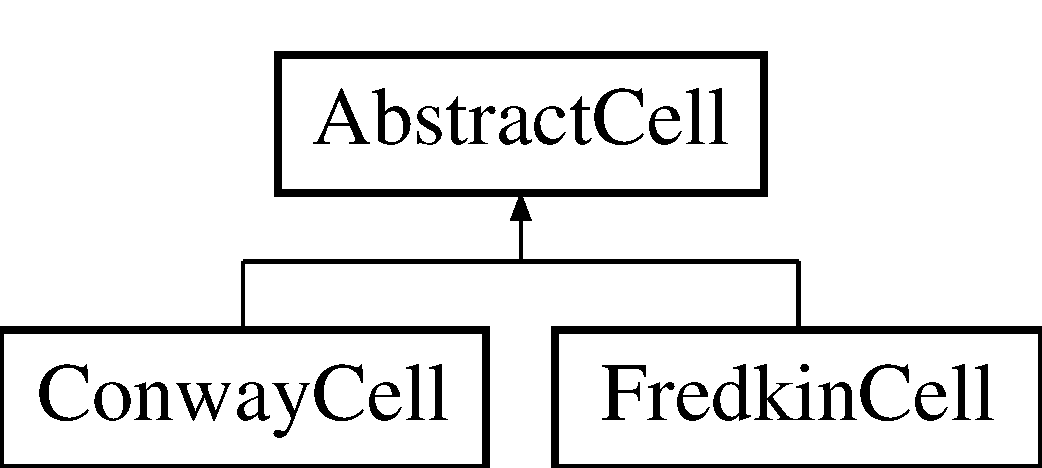
\includegraphics[height=2.000000cm]{classAbstractCell}
\end{center}
\end{figure}
\subsection*{Public Member Functions}
\begin{DoxyCompactItemize}
\item 
\hyperlink{classAbstractCell_af753342773dbd879161d9c9b1afe9874}{Abstract\-Cell} (bool alived)
\item 
\hyperlink{classAbstractCell_a92a128eb6dbabbdcfba8973503aea71e}{Abstract\-Cell} (const \hyperlink{classAbstractCell}{Abstract\-Cell} \&)=default
\item 
\hyperlink{classAbstractCell_ad8eea1ec8c279add40136cd28db11e97}{Abstract\-Cell} (\hyperlink{classAbstractCell}{Abstract\-Cell} \&\&)=default
\item 
virtual \hyperlink{classAbstractCell_a6d8ce67b93514f1fc2f564a7bb09cf85}{$\sim$\-Abstract\-Cell} ()=default
\item 
virtual \hyperlink{classAbstractCell}{Abstract\-Cell} $\ast$ \hyperlink{classAbstractCell_a1a95a7ea92b3503e2f042170b6320354}{clone} () const =0
\item 
virtual void \hyperlink{classAbstractCell_a67008aedffea84aac7088ec84e8441cc}{update\-\_\-state} (string c)=0
\item 
virtual int \hyperlink{classAbstractCell_af566abaafe33b73bae0874566a987b63}{count\-\_\-neighbor} (int possible\-\_\-nb\mbox{[}$\,$\mbox{]}) const =0
\item 
virtual string \hyperlink{classAbstractCell_a63e875724c1ee0278449d9489211baa7}{print} ()=0
\item 
virtual void \hyperlink{classAbstractCell_ad46c73f9a67419ecd570a7677525054f}{evolve} (int num\-\_\-neighbors)=0
\item 
virtual int \hyperlink{classAbstractCell_aac03c6e21580569ae306909e68feae9d}{cnt} ()=0
\item 
virtual bool \hyperlink{classAbstractCell_a9eb218c97afe5618c8e2783335cc425c}{operator==} (const \hyperlink{classAbstractCell}{Abstract\-Cell} \&rhs) const 
\item 
\hyperlink{classAbstractCell_a60254ac736576a6645b6863926f86fc1}{F\-R\-I\-E\-N\-D\-\_\-\-T\-E\-S\-T} (\hyperlink{classAbstractCell_a8a83d646164e396527131ba80ec82bdc}{Abstract\-Cell\-Test}, Abstract\-Cell\-\_\-1)
\item 
\hyperlink{classAbstractCell_a1c4e29381db068d39eac4a103587151f}{F\-R\-I\-E\-N\-D\-\_\-\-T\-E\-S\-T} (\hyperlink{classAbstractCell_a8a83d646164e396527131ba80ec82bdc}{Abstract\-Cell\-Test}, Abstract\-Cell\-\_\-2)
\item 
\hyperlink{classAbstractCell_a126d29fd8943e3b611d51842a4d4de53}{F\-R\-I\-E\-N\-D\-\_\-\-T\-E\-S\-T} (\hyperlink{classAbstractCell_a8a83d646164e396527131ba80ec82bdc}{Abstract\-Cell\-Test}, Abstract\-Cell\-\_\-3)
\item 
\hyperlink{classAbstractCell_a28b9bfbf4fcfa5ee7b2f0e6cdbfba7d6}{F\-R\-I\-E\-N\-D\-\_\-\-T\-E\-S\-T} (\hyperlink{classAbstractCell_a8a83d646164e396527131ba80ec82bdc}{Abstract\-Cell\-Test}, operator\-\_\-equal\-\_\-equal\-\_\-1)
\item 
\hyperlink{classAbstractCell_a5f5173debbe09a8a170f7f61861cc397}{F\-R\-I\-E\-N\-D\-\_\-\-T\-E\-S\-T} (\hyperlink{classAbstractCell_a8a83d646164e396527131ba80ec82bdc}{Abstract\-Cell\-Test}, operator\-\_\-equal\-\_\-equal\-\_\-2)
\item 
\hyperlink{classAbstractCell_a1fd4de21840d045a818c699c5f812f61}{F\-R\-I\-E\-N\-D\-\_\-\-T\-E\-S\-T} (\hyperlink{classAbstractCell_a8a83d646164e396527131ba80ec82bdc}{Abstract\-Cell\-Test}, operator\-\_\-equal\-\_\-equal\-\_\-3)
\end{DoxyCompactItemize}
\subsection*{Protected Member Functions}
\begin{DoxyCompactItemize}
\item 
\hyperlink{classAbstractCell}{Abstract\-Cell} \& \hyperlink{classAbstractCell_ac24aa175a3d52191df86a7d1aefb85c5}{operator=} (const \hyperlink{classAbstractCell}{Abstract\-Cell} \&)=default
\item 
\hyperlink{classAbstractCell}{Abstract\-Cell} \& \hyperlink{classAbstractCell_a82608116be17096641ce4aa5cffe1018}{operator=} (\hyperlink{classAbstractCell}{Abstract\-Cell} \&\&)=default
\end{DoxyCompactItemize}
\subsection*{Protected Attributes}
\begin{DoxyCompactItemize}
\item 
bool \hyperlink{classAbstractCell_abdd4785483cace729e7fee7a1e53848c}{\-\_\-alived}
\end{DoxyCompactItemize}
\subsection*{Friends}
\begin{DoxyCompactItemize}
\item 
class \hyperlink{classAbstractCell_a8a83d646164e396527131ba80ec82bdc}{Abstract\-Cell\-Test}
\end{DoxyCompactItemize}


\subsection{Constructor \& Destructor Documentation}
\hypertarget{classAbstractCell_af753342773dbd879161d9c9b1afe9874}{\index{Abstract\-Cell@{Abstract\-Cell}!Abstract\-Cell@{Abstract\-Cell}}
\index{Abstract\-Cell@{Abstract\-Cell}!AbstractCell@{Abstract\-Cell}}
\subsubsection[{Abstract\-Cell}]{\setlength{\rightskip}{0pt plus 5cm}Abstract\-Cell\-::\-Abstract\-Cell (
\begin{DoxyParamCaption}
\item[{bool}]{alived}
\end{DoxyParamCaption}
)}}\label{classAbstractCell_af753342773dbd879161d9c9b1afe9874}
\hypertarget{classAbstractCell_a92a128eb6dbabbdcfba8973503aea71e}{\index{Abstract\-Cell@{Abstract\-Cell}!Abstract\-Cell@{Abstract\-Cell}}
\index{Abstract\-Cell@{Abstract\-Cell}!AbstractCell@{Abstract\-Cell}}
\subsubsection[{Abstract\-Cell}]{\setlength{\rightskip}{0pt plus 5cm}Abstract\-Cell\-::\-Abstract\-Cell (
\begin{DoxyParamCaption}
\item[{const {\bf Abstract\-Cell} \&}]{}
\end{DoxyParamCaption}
)\hspace{0.3cm}{\ttfamily [default]}}}\label{classAbstractCell_a92a128eb6dbabbdcfba8973503aea71e}
\hypertarget{classAbstractCell_ad8eea1ec8c279add40136cd28db11e97}{\index{Abstract\-Cell@{Abstract\-Cell}!Abstract\-Cell@{Abstract\-Cell}}
\index{Abstract\-Cell@{Abstract\-Cell}!AbstractCell@{Abstract\-Cell}}
\subsubsection[{Abstract\-Cell}]{\setlength{\rightskip}{0pt plus 5cm}Abstract\-Cell\-::\-Abstract\-Cell (
\begin{DoxyParamCaption}
\item[{{\bf Abstract\-Cell} \&\&}]{}
\end{DoxyParamCaption}
)\hspace{0.3cm}{\ttfamily [default]}}}\label{classAbstractCell_ad8eea1ec8c279add40136cd28db11e97}
\hypertarget{classAbstractCell_a6d8ce67b93514f1fc2f564a7bb09cf85}{\index{Abstract\-Cell@{Abstract\-Cell}!$\sim$\-Abstract\-Cell@{$\sim$\-Abstract\-Cell}}
\index{$\sim$\-Abstract\-Cell@{$\sim$\-Abstract\-Cell}!AbstractCell@{Abstract\-Cell}}
\subsubsection[{$\sim$\-Abstract\-Cell}]{\setlength{\rightskip}{0pt plus 5cm}virtual Abstract\-Cell\-::$\sim$\-Abstract\-Cell (
\begin{DoxyParamCaption}
{}
\end{DoxyParamCaption}
)\hspace{0.3cm}{\ttfamily [virtual]}, {\ttfamily [default]}}}\label{classAbstractCell_a6d8ce67b93514f1fc2f564a7bb09cf85}


\subsection{Member Function Documentation}
\hypertarget{classAbstractCell_a1a95a7ea92b3503e2f042170b6320354}{\index{Abstract\-Cell@{Abstract\-Cell}!clone@{clone}}
\index{clone@{clone}!AbstractCell@{Abstract\-Cell}}
\subsubsection[{clone}]{\setlength{\rightskip}{0pt plus 5cm}virtual {\bf Abstract\-Cell}$\ast$ Abstract\-Cell\-::clone (
\begin{DoxyParamCaption}
{}
\end{DoxyParamCaption}
) const\hspace{0.3cm}{\ttfamily [pure virtual]}}}\label{classAbstractCell_a1a95a7ea92b3503e2f042170b6320354}


Implemented in \hyperlink{classFredkinCell_a89984e2ceee786e199f3d5cd5ab46536}{Fredkin\-Cell}, and \hyperlink{classConwayCell_a00e3f8117929e7dcbb85f71aeaa10368}{Conway\-Cell}.

\hypertarget{classAbstractCell_aac03c6e21580569ae306909e68feae9d}{\index{Abstract\-Cell@{Abstract\-Cell}!cnt@{cnt}}
\index{cnt@{cnt}!AbstractCell@{Abstract\-Cell}}
\subsubsection[{cnt}]{\setlength{\rightskip}{0pt plus 5cm}virtual int Abstract\-Cell\-::cnt (
\begin{DoxyParamCaption}
{}
\end{DoxyParamCaption}
)\hspace{0.3cm}{\ttfamily [pure virtual]}}}\label{classAbstractCell_aac03c6e21580569ae306909e68feae9d}
\begin{DoxyReturn}{Returns}
count 1 for alived, count 0 for dead 
\end{DoxyReturn}


Implemented in \hyperlink{classFredkinCell_a9721fe3c5efbb6abc6feabdbde7069cf}{Fredkin\-Cell}, and \hyperlink{classConwayCell_a49c7cf05666f19c89e8a0b29a78a6d3f}{Conway\-Cell}.

\hypertarget{classAbstractCell_af566abaafe33b73bae0874566a987b63}{\index{Abstract\-Cell@{Abstract\-Cell}!count\-\_\-neighbor@{count\-\_\-neighbor}}
\index{count\-\_\-neighbor@{count\-\_\-neighbor}!AbstractCell@{Abstract\-Cell}}
\subsubsection[{count\-\_\-neighbor}]{\setlength{\rightskip}{0pt plus 5cm}virtual int Abstract\-Cell\-::count\-\_\-neighbor (
\begin{DoxyParamCaption}
\item[{int}]{possible\-\_\-nb\mbox{[}$\,$\mbox{]}}
\end{DoxyParamCaption}
) const\hspace{0.3cm}{\ttfamily [pure virtual]}}}\label{classAbstractCell_af566abaafe33b73bae0874566a987b63}

\begin{DoxyParams}{Parameters}
{\em int\mbox{[}$\,$\mbox{]}} & of possible neighbors upto 8 neighbors \\
\hline
\end{DoxyParams}
\begin{DoxyReturn}{Returns}
int number of neighbor 
\end{DoxyReturn}


Implemented in \hyperlink{classFredkinCell_a695f37645d14ba1faa11518a70b3351a}{Fredkin\-Cell}, and \hyperlink{classConwayCell_afbd79c8a5fc7a7da5885cdc7445f5b45}{Conway\-Cell}.

\hypertarget{classAbstractCell_ad46c73f9a67419ecd570a7677525054f}{\index{Abstract\-Cell@{Abstract\-Cell}!evolve@{evolve}}
\index{evolve@{evolve}!AbstractCell@{Abstract\-Cell}}
\subsubsection[{evolve}]{\setlength{\rightskip}{0pt plus 5cm}virtual void Abstract\-Cell\-::evolve (
\begin{DoxyParamCaption}
\item[{int}]{num\-\_\-neighbors}
\end{DoxyParamCaption}
)\hspace{0.3cm}{\ttfamily [pure virtual]}}}\label{classAbstractCell_ad46c73f9a67419ecd570a7677525054f}

\begin{DoxyParams}{Parameters}
{\em int} & number of neighbors \\
\hline
\end{DoxyParams}


Implemented in \hyperlink{classFredkinCell_acd5eb2ee81b8ba40cd943c5c6ed638bc}{Fredkin\-Cell}, and \hyperlink{classConwayCell_a94a403a65aac5b0c9fd69c175122151c}{Conway\-Cell}.

\hypertarget{classAbstractCell_a60254ac736576a6645b6863926f86fc1}{\index{Abstract\-Cell@{Abstract\-Cell}!F\-R\-I\-E\-N\-D\-\_\-\-T\-E\-S\-T@{F\-R\-I\-E\-N\-D\-\_\-\-T\-E\-S\-T}}
\index{F\-R\-I\-E\-N\-D\-\_\-\-T\-E\-S\-T@{F\-R\-I\-E\-N\-D\-\_\-\-T\-E\-S\-T}!AbstractCell@{Abstract\-Cell}}
\subsubsection[{F\-R\-I\-E\-N\-D\-\_\-\-T\-E\-S\-T}]{\setlength{\rightskip}{0pt plus 5cm}Abstract\-Cell\-::\-F\-R\-I\-E\-N\-D\-\_\-\-T\-E\-S\-T (
\begin{DoxyParamCaption}
\item[{{\bf Abstract\-Cell\-Test}}]{, }
\item[{Abstract\-Cell\-\_\-1}]{}
\end{DoxyParamCaption}
)}}\label{classAbstractCell_a60254ac736576a6645b6863926f86fc1}
\hypertarget{classAbstractCell_a1c4e29381db068d39eac4a103587151f}{\index{Abstract\-Cell@{Abstract\-Cell}!F\-R\-I\-E\-N\-D\-\_\-\-T\-E\-S\-T@{F\-R\-I\-E\-N\-D\-\_\-\-T\-E\-S\-T}}
\index{F\-R\-I\-E\-N\-D\-\_\-\-T\-E\-S\-T@{F\-R\-I\-E\-N\-D\-\_\-\-T\-E\-S\-T}!AbstractCell@{Abstract\-Cell}}
\subsubsection[{F\-R\-I\-E\-N\-D\-\_\-\-T\-E\-S\-T}]{\setlength{\rightskip}{0pt plus 5cm}Abstract\-Cell\-::\-F\-R\-I\-E\-N\-D\-\_\-\-T\-E\-S\-T (
\begin{DoxyParamCaption}
\item[{{\bf Abstract\-Cell\-Test}}]{, }
\item[{Abstract\-Cell\-\_\-2}]{}
\end{DoxyParamCaption}
)}}\label{classAbstractCell_a1c4e29381db068d39eac4a103587151f}
\hypertarget{classAbstractCell_a126d29fd8943e3b611d51842a4d4de53}{\index{Abstract\-Cell@{Abstract\-Cell}!F\-R\-I\-E\-N\-D\-\_\-\-T\-E\-S\-T@{F\-R\-I\-E\-N\-D\-\_\-\-T\-E\-S\-T}}
\index{F\-R\-I\-E\-N\-D\-\_\-\-T\-E\-S\-T@{F\-R\-I\-E\-N\-D\-\_\-\-T\-E\-S\-T}!AbstractCell@{Abstract\-Cell}}
\subsubsection[{F\-R\-I\-E\-N\-D\-\_\-\-T\-E\-S\-T}]{\setlength{\rightskip}{0pt plus 5cm}Abstract\-Cell\-::\-F\-R\-I\-E\-N\-D\-\_\-\-T\-E\-S\-T (
\begin{DoxyParamCaption}
\item[{{\bf Abstract\-Cell\-Test}}]{, }
\item[{Abstract\-Cell\-\_\-3}]{}
\end{DoxyParamCaption}
)}}\label{classAbstractCell_a126d29fd8943e3b611d51842a4d4de53}
\hypertarget{classAbstractCell_a28b9bfbf4fcfa5ee7b2f0e6cdbfba7d6}{\index{Abstract\-Cell@{Abstract\-Cell}!F\-R\-I\-E\-N\-D\-\_\-\-T\-E\-S\-T@{F\-R\-I\-E\-N\-D\-\_\-\-T\-E\-S\-T}}
\index{F\-R\-I\-E\-N\-D\-\_\-\-T\-E\-S\-T@{F\-R\-I\-E\-N\-D\-\_\-\-T\-E\-S\-T}!AbstractCell@{Abstract\-Cell}}
\subsubsection[{F\-R\-I\-E\-N\-D\-\_\-\-T\-E\-S\-T}]{\setlength{\rightskip}{0pt plus 5cm}Abstract\-Cell\-::\-F\-R\-I\-E\-N\-D\-\_\-\-T\-E\-S\-T (
\begin{DoxyParamCaption}
\item[{{\bf Abstract\-Cell\-Test}}]{, }
\item[{operator\-\_\-equal\-\_\-equal\-\_\-1}]{}
\end{DoxyParamCaption}
)}}\label{classAbstractCell_a28b9bfbf4fcfa5ee7b2f0e6cdbfba7d6}
\hypertarget{classAbstractCell_a5f5173debbe09a8a170f7f61861cc397}{\index{Abstract\-Cell@{Abstract\-Cell}!F\-R\-I\-E\-N\-D\-\_\-\-T\-E\-S\-T@{F\-R\-I\-E\-N\-D\-\_\-\-T\-E\-S\-T}}
\index{F\-R\-I\-E\-N\-D\-\_\-\-T\-E\-S\-T@{F\-R\-I\-E\-N\-D\-\_\-\-T\-E\-S\-T}!AbstractCell@{Abstract\-Cell}}
\subsubsection[{F\-R\-I\-E\-N\-D\-\_\-\-T\-E\-S\-T}]{\setlength{\rightskip}{0pt plus 5cm}Abstract\-Cell\-::\-F\-R\-I\-E\-N\-D\-\_\-\-T\-E\-S\-T (
\begin{DoxyParamCaption}
\item[{{\bf Abstract\-Cell\-Test}}]{, }
\item[{operator\-\_\-equal\-\_\-equal\-\_\-2}]{}
\end{DoxyParamCaption}
)}}\label{classAbstractCell_a5f5173debbe09a8a170f7f61861cc397}
\hypertarget{classAbstractCell_a1fd4de21840d045a818c699c5f812f61}{\index{Abstract\-Cell@{Abstract\-Cell}!F\-R\-I\-E\-N\-D\-\_\-\-T\-E\-S\-T@{F\-R\-I\-E\-N\-D\-\_\-\-T\-E\-S\-T}}
\index{F\-R\-I\-E\-N\-D\-\_\-\-T\-E\-S\-T@{F\-R\-I\-E\-N\-D\-\_\-\-T\-E\-S\-T}!AbstractCell@{Abstract\-Cell}}
\subsubsection[{F\-R\-I\-E\-N\-D\-\_\-\-T\-E\-S\-T}]{\setlength{\rightskip}{0pt plus 5cm}Abstract\-Cell\-::\-F\-R\-I\-E\-N\-D\-\_\-\-T\-E\-S\-T (
\begin{DoxyParamCaption}
\item[{{\bf Abstract\-Cell\-Test}}]{, }
\item[{operator\-\_\-equal\-\_\-equal\-\_\-3}]{}
\end{DoxyParamCaption}
)}}\label{classAbstractCell_a1fd4de21840d045a818c699c5f812f61}
\hypertarget{classAbstractCell_ac24aa175a3d52191df86a7d1aefb85c5}{\index{Abstract\-Cell@{Abstract\-Cell}!operator=@{operator=}}
\index{operator=@{operator=}!AbstractCell@{Abstract\-Cell}}
\subsubsection[{operator=}]{\setlength{\rightskip}{0pt plus 5cm}{\bf Abstract\-Cell}\& Abstract\-Cell\-::operator= (
\begin{DoxyParamCaption}
\item[{const {\bf Abstract\-Cell} \&}]{}
\end{DoxyParamCaption}
)\hspace{0.3cm}{\ttfamily [protected]}, {\ttfamily [default]}}}\label{classAbstractCell_ac24aa175a3d52191df86a7d1aefb85c5}
\hypertarget{classAbstractCell_a82608116be17096641ce4aa5cffe1018}{\index{Abstract\-Cell@{Abstract\-Cell}!operator=@{operator=}}
\index{operator=@{operator=}!AbstractCell@{Abstract\-Cell}}
\subsubsection[{operator=}]{\setlength{\rightskip}{0pt plus 5cm}{\bf Abstract\-Cell}\& Abstract\-Cell\-::operator= (
\begin{DoxyParamCaption}
\item[{{\bf Abstract\-Cell} \&\&}]{}
\end{DoxyParamCaption}
)\hspace{0.3cm}{\ttfamily [protected]}, {\ttfamily [default]}}}\label{classAbstractCell_a82608116be17096641ce4aa5cffe1018}
\hypertarget{classAbstractCell_a9eb218c97afe5618c8e2783335cc425c}{\index{Abstract\-Cell@{Abstract\-Cell}!operator==@{operator==}}
\index{operator==@{operator==}!AbstractCell@{Abstract\-Cell}}
\subsubsection[{operator==}]{\setlength{\rightskip}{0pt plus 5cm}bool Abstract\-Cell\-::operator== (
\begin{DoxyParamCaption}
\item[{const {\bf Abstract\-Cell} \&}]{rhs}
\end{DoxyParamCaption}
) const\hspace{0.3cm}{\ttfamily [virtual]}}}\label{classAbstractCell_a9eb218c97afe5618c8e2783335cc425c}

\begin{DoxyParams}{Parameters}
{\em other} & \hyperlink{classAbstractCell}{Abstract\-Cell} \\
\hline
\end{DoxyParams}
\begin{DoxyReturn}{Returns}
true for equal, otherwise false 
\end{DoxyReturn}
\hypertarget{classAbstractCell_a63e875724c1ee0278449d9489211baa7}{\index{Abstract\-Cell@{Abstract\-Cell}!print@{print}}
\index{print@{print}!AbstractCell@{Abstract\-Cell}}
\subsubsection[{print}]{\setlength{\rightskip}{0pt plus 5cm}virtual string Abstract\-Cell\-::print (
\begin{DoxyParamCaption}
{}
\end{DoxyParamCaption}
)\hspace{0.3cm}{\ttfamily [pure virtual]}}}\label{classAbstractCell_a63e875724c1ee0278449d9489211baa7}

\begin{DoxyParams}{Parameters}
{\em @return} & string character of the cell state \\
\hline
\end{DoxyParams}


Implemented in \hyperlink{classFredkinCell_a54ba3c20d52deebd57c557748cd36bb8}{Fredkin\-Cell}, and \hyperlink{classConwayCell_ad8be337992eca64445ebc1259af8d4ca}{Conway\-Cell}.

\hypertarget{classAbstractCell_a67008aedffea84aac7088ec84e8441cc}{\index{Abstract\-Cell@{Abstract\-Cell}!update\-\_\-state@{update\-\_\-state}}
\index{update\-\_\-state@{update\-\_\-state}!AbstractCell@{Abstract\-Cell}}
\subsubsection[{update\-\_\-state}]{\setlength{\rightskip}{0pt plus 5cm}virtual void Abstract\-Cell\-::update\-\_\-state (
\begin{DoxyParamCaption}
\item[{string}]{c}
\end{DoxyParamCaption}
)\hspace{0.3cm}{\ttfamily [pure virtual]}}}\label{classAbstractCell_a67008aedffea84aac7088ec84e8441cc}

\begin{DoxyParams}{Parameters}
{\em String} & character \\
\hline
\end{DoxyParams}


Implemented in \hyperlink{classFredkinCell_a55fa842b999a1293d08be7d3a75cb537}{Fredkin\-Cell}, and \hyperlink{classConwayCell_a6a0d34c7f90a1b76e144c891ba4541e5}{Conway\-Cell}.



\subsection{Friends And Related Function Documentation}
\hypertarget{classAbstractCell_a8a83d646164e396527131ba80ec82bdc}{\index{Abstract\-Cell@{Abstract\-Cell}!Abstract\-Cell\-Test@{Abstract\-Cell\-Test}}
\index{Abstract\-Cell\-Test@{Abstract\-Cell\-Test}!AbstractCell@{Abstract\-Cell}}
\subsubsection[{Abstract\-Cell\-Test}]{\setlength{\rightskip}{0pt plus 5cm}friend class Abstract\-Cell\-Test\hspace{0.3cm}{\ttfamily [friend]}}}\label{classAbstractCell_a8a83d646164e396527131ba80ec82bdc}


\subsection{Member Data Documentation}
\hypertarget{classAbstractCell_abdd4785483cace729e7fee7a1e53848c}{\index{Abstract\-Cell@{Abstract\-Cell}!\-\_\-alived@{\-\_\-alived}}
\index{\-\_\-alived@{\-\_\-alived}!AbstractCell@{Abstract\-Cell}}
\subsubsection[{\-\_\-alived}]{\setlength{\rightskip}{0pt plus 5cm}bool Abstract\-Cell\-::\-\_\-alived\hspace{0.3cm}{\ttfamily [protected]}}}\label{classAbstractCell_abdd4785483cace729e7fee7a1e53848c}


The documentation for this class was generated from the following files\-:\begin{DoxyCompactItemize}
\item 
\hyperlink{Life_8h}{Life.\-h}\item 
\hyperlink{Life_8c_09_09}{Life.\-c++}\end{DoxyCompactItemize}

\hypertarget{classCell}{\section{Cell Class Reference}
\label{classCell}\index{Cell@{Cell}}
}


{\ttfamily \#include $<$Life.\-h$>$}

\subsection*{Public Member Functions}
\begin{DoxyCompactItemize}
\item 
\hyperlink{classCell_a394510643e8664cf12b5efaf5cb99f71}{Cell} ()
\item 
\hyperlink{classCell_a8ca000885181236a713963c5c8bdb46f}{Cell} (const \hyperlink{classCell}{Cell} \&)
\item 
\hyperlink{classCell_a07dc1c921001f28dfd83cc2511c913ed}{Cell} (\hyperlink{classCell}{Cell} \&\&)=default
\item 
\hyperlink{classCell}{Cell} \& \hyperlink{classCell_a45915eabf6c5940c10bc05112c16fb91}{operator=} (const \hyperlink{classCell}{Cell} \&)=default
\item 
\hyperlink{classCell}{Cell} \& \hyperlink{classCell_a87fc42eae25a2ef5e982804646108df8}{operator=} (\hyperlink{classCell}{Cell} \&\&)=default
\item 
\hyperlink{classCell_a9fa559f7a28e2b4336c6879ca09304d8}{$\sim$\-Cell} ()
\item 
void \hyperlink{classCell_ae33f6e56c2c45696eb2fa5ef3d431e79}{update\-\_\-state} (string c)
\item 
int \hyperlink{classCell_a16143f59210233e77fb2e883584f62d0}{count\-\_\-neighbor} (int possible\-\_\-nb\mbox{[}$\,$\mbox{]}) const 
\item 
string \hyperlink{classCell_a00ae4bdf312b9a5ba5b505b3ed9d7731}{print} ()
\item 
void \hyperlink{classCell_a7eb57e91d1244ef230efdaa1e4707007}{evolve} (int num\-\_\-neighbors)
\item 
int \hyperlink{classCell_a819661c780e31c3c0b69d084c1e06577}{cnt} ()
\item 
bool \hyperlink{classCell_a4c1ef917de3d6aae865d13ddb590a607}{operator==} (const \hyperlink{classCell}{Cell} \&rhs) const 
\item 
\hyperlink{classCell_a8c4981431d8778737227d412d953ced4}{F\-R\-I\-E\-N\-D\-\_\-\-T\-E\-S\-T} (\hyperlink{classCell_a4a8fb13b6ff304aefc7aa29538062941}{Cell\-Test}, Cell\-\_\-1)
\item 
\hyperlink{classCell_ac7a28dab71b04608f6ba9bc9e4dd22b5}{F\-R\-I\-E\-N\-D\-\_\-\-T\-E\-S\-T} (\hyperlink{classCell_a4a8fb13b6ff304aefc7aa29538062941}{Cell\-Test}, Cell\-\_\-2)
\item 
\hyperlink{classCell_a9583f761975928f9a3e8b07174fb40ef}{F\-R\-I\-E\-N\-D\-\_\-\-T\-E\-S\-T} (\hyperlink{classCell_a4a8fb13b6ff304aefc7aa29538062941}{Cell\-Test}, Cell\-\_\-3)
\item 
\hyperlink{classCell_ab60670aa7385b6cf5ae13f8a26743b8d}{F\-R\-I\-E\-N\-D\-\_\-\-T\-E\-S\-T} (\hyperlink{classCell_a4a8fb13b6ff304aefc7aa29538062941}{Cell\-Test}, clone\-\_\-1)
\item 
\hyperlink{classCell_a019c5da45cec2255da2c4ab0d7805ec5}{F\-R\-I\-E\-N\-D\-\_\-\-T\-E\-S\-T} (\hyperlink{classCell_a4a8fb13b6ff304aefc7aa29538062941}{Cell\-Test}, clone\-\_\-2)
\item 
\hyperlink{classCell_a502208a79c44f6601e157a1dcdcac4d1}{F\-R\-I\-E\-N\-D\-\_\-\-T\-E\-S\-T} (\hyperlink{classCell_a4a8fb13b6ff304aefc7aa29538062941}{Cell\-Test}, clone\-\_\-3)
\item 
\hyperlink{classCell_aa5ea305159c8c7b067286cda4e828218}{F\-R\-I\-E\-N\-D\-\_\-\-T\-E\-S\-T} (\hyperlink{classCell_a4a8fb13b6ff304aefc7aa29538062941}{Cell\-Test}, update\-\_\-state\-\_\-1)
\item 
\hyperlink{classCell_a8928f24da1d3b7ab13be5f027636c495}{F\-R\-I\-E\-N\-D\-\_\-\-T\-E\-S\-T} (\hyperlink{classCell_a4a8fb13b6ff304aefc7aa29538062941}{Cell\-Test}, update\-\_\-state\-\_\-2)
\item 
\hyperlink{classCell_a35d41917a03645cf9d75edde241d6752}{F\-R\-I\-E\-N\-D\-\_\-\-T\-E\-S\-T} (\hyperlink{classCell_a4a8fb13b6ff304aefc7aa29538062941}{Cell\-Test}, update\-\_\-state\-\_\-3)
\item 
\hyperlink{classCell_a4e6cadd65d76a1a4223e1ce2f5a0a32b}{F\-R\-I\-E\-N\-D\-\_\-\-T\-E\-S\-T} (\hyperlink{classCell_a4a8fb13b6ff304aefc7aa29538062941}{Cell\-Test}, count\-\_\-neighbor\-\_\-1)
\item 
\hyperlink{classCell_ab813fa2df3240553c36e5ed8a2fb7c57}{F\-R\-I\-E\-N\-D\-\_\-\-T\-E\-S\-T} (\hyperlink{classCell_a4a8fb13b6ff304aefc7aa29538062941}{Cell\-Test}, count\-\_\-neighbor\-\_\-2)
\item 
\hyperlink{classCell_a865fe812b0dfd098462752fb1a561b44}{F\-R\-I\-E\-N\-D\-\_\-\-T\-E\-S\-T} (\hyperlink{classCell_a4a8fb13b6ff304aefc7aa29538062941}{Cell\-Test}, count\-\_\-neighbor\-\_\-3)
\item 
\hyperlink{classCell_adff24a73ddfdcb0fb212706ed1f0b0ab}{F\-R\-I\-E\-N\-D\-\_\-\-T\-E\-S\-T} (\hyperlink{classCell_a4a8fb13b6ff304aefc7aa29538062941}{Cell\-Test}, print\-\_\-1)
\item 
\hyperlink{classCell_a5bc3951f0c503da404ee6c6863e819fb}{F\-R\-I\-E\-N\-D\-\_\-\-T\-E\-S\-T} (\hyperlink{classCell_a4a8fb13b6ff304aefc7aa29538062941}{Cell\-Test}, print\-\_\-2)
\item 
\hyperlink{classCell_a70a0ef17fcc23ffbb87deab727075268}{F\-R\-I\-E\-N\-D\-\_\-\-T\-E\-S\-T} (\hyperlink{classCell_a4a8fb13b6ff304aefc7aa29538062941}{Cell\-Test}, print\-\_\-3)
\item 
\hyperlink{classCell_a824557ceb650e5c124567a64bc5c6e4f}{F\-R\-I\-E\-N\-D\-\_\-\-T\-E\-S\-T} (\hyperlink{classCell_a4a8fb13b6ff304aefc7aa29538062941}{Cell\-Test}, evolve\-\_\-1)
\item 
\hyperlink{classCell_a2ac0a81f96898596cdd2711ee5880ff4}{F\-R\-I\-E\-N\-D\-\_\-\-T\-E\-S\-T} (\hyperlink{classCell_a4a8fb13b6ff304aefc7aa29538062941}{Cell\-Test}, evolve\-\_\-2)
\item 
\hyperlink{classCell_af0edc16195146ce5755e13df3c2db294}{F\-R\-I\-E\-N\-D\-\_\-\-T\-E\-S\-T} (\hyperlink{classCell_a4a8fb13b6ff304aefc7aa29538062941}{Cell\-Test}, evolve\-\_\-3)
\item 
\hyperlink{classCell_a7e7750ebadd0abf2b2b51e42262c0c97}{F\-R\-I\-E\-N\-D\-\_\-\-T\-E\-S\-T} (\hyperlink{classCell_a4a8fb13b6ff304aefc7aa29538062941}{Cell\-Test}, cnt\-\_\-1)
\item 
\hyperlink{classCell_a584061321fadade7c6a41400bde406ff}{F\-R\-I\-E\-N\-D\-\_\-\-T\-E\-S\-T} (\hyperlink{classCell_a4a8fb13b6ff304aefc7aa29538062941}{Cell\-Test}, cnt\-\_\-2)
\item 
\hyperlink{classCell_aaf4702292ab380ee439ff51e4b1d46e8}{F\-R\-I\-E\-N\-D\-\_\-\-T\-E\-S\-T} (\hyperlink{classCell_a4a8fb13b6ff304aefc7aa29538062941}{Cell\-Test}, cnt\-\_\-3)
\end{DoxyCompactItemize}
\subsection*{Private Attributes}
\begin{DoxyCompactItemize}
\item 
\hyperlink{classAbstractCell}{Abstract\-Cell} $\ast$ \hyperlink{classCell_af8bb6306c15463d257e4775095b2f273}{\-\_\-p}
\end{DoxyCompactItemize}
\subsection*{Friends}
\begin{DoxyCompactItemize}
\item 
class \hyperlink{classCell_a4a8fb13b6ff304aefc7aa29538062941}{Cell\-Test}
\end{DoxyCompactItemize}


\subsection{Constructor \& Destructor Documentation}
\hypertarget{classCell_a394510643e8664cf12b5efaf5cb99f71}{\index{Cell@{Cell}!Cell@{Cell}}
\index{Cell@{Cell}!Cell@{Cell}}
\subsubsection[{Cell}]{\setlength{\rightskip}{0pt plus 5cm}Cell\-::\-Cell (
\begin{DoxyParamCaption}
{}
\end{DoxyParamCaption}
)}}\label{classCell_a394510643e8664cf12b5efaf5cb99f71}

\begin{DoxyParams}{Parameters}
{\em String} & name and default \\
\hline
\end{DoxyParams}
\hypertarget{classCell_a8ca000885181236a713963c5c8bdb46f}{\index{Cell@{Cell}!Cell@{Cell}}
\index{Cell@{Cell}!Cell@{Cell}}
\subsubsection[{Cell}]{\setlength{\rightskip}{0pt plus 5cm}Cell\-::\-Cell (
\begin{DoxyParamCaption}
\item[{const {\bf Cell} \&}]{rhs}
\end{DoxyParamCaption}
)}}\label{classCell_a8ca000885181236a713963c5c8bdb46f}
\hypertarget{classCell_a07dc1c921001f28dfd83cc2511c913ed}{\index{Cell@{Cell}!Cell@{Cell}}
\index{Cell@{Cell}!Cell@{Cell}}
\subsubsection[{Cell}]{\setlength{\rightskip}{0pt plus 5cm}Cell\-::\-Cell (
\begin{DoxyParamCaption}
\item[{{\bf Cell} \&\&}]{}
\end{DoxyParamCaption}
)\hspace{0.3cm}{\ttfamily [default]}}}\label{classCell_a07dc1c921001f28dfd83cc2511c913ed}
\hypertarget{classCell_a9fa559f7a28e2b4336c6879ca09304d8}{\index{Cell@{Cell}!$\sim$\-Cell@{$\sim$\-Cell}}
\index{$\sim$\-Cell@{$\sim$\-Cell}!Cell@{Cell}}
\subsubsection[{$\sim$\-Cell}]{\setlength{\rightskip}{0pt plus 5cm}Cell\-::$\sim$\-Cell (
\begin{DoxyParamCaption}
{}
\end{DoxyParamCaption}
)}}\label{classCell_a9fa559f7a28e2b4336c6879ca09304d8}

\begin{DoxyParams}{Parameters}
{\em String} & name and default \\
\hline
\end{DoxyParams}


\subsection{Member Function Documentation}
\hypertarget{classCell_a819661c780e31c3c0b69d084c1e06577}{\index{Cell@{Cell}!cnt@{cnt}}
\index{cnt@{cnt}!Cell@{Cell}}
\subsubsection[{cnt}]{\setlength{\rightskip}{0pt plus 5cm}int Cell\-::cnt (
\begin{DoxyParamCaption}
{}
\end{DoxyParamCaption}
)}}\label{classCell_a819661c780e31c3c0b69d084c1e06577}
\begin{DoxyReturn}{Returns}
count 1 for alived, count 0 for dead 
\end{DoxyReturn}
\hypertarget{classCell_a16143f59210233e77fb2e883584f62d0}{\index{Cell@{Cell}!count\-\_\-neighbor@{count\-\_\-neighbor}}
\index{count\-\_\-neighbor@{count\-\_\-neighbor}!Cell@{Cell}}
\subsubsection[{count\-\_\-neighbor}]{\setlength{\rightskip}{0pt plus 5cm}int Cell\-::count\-\_\-neighbor (
\begin{DoxyParamCaption}
\item[{int}]{possible\-\_\-nb\mbox{[}$\,$\mbox{]}}
\end{DoxyParamCaption}
) const}}\label{classCell_a16143f59210233e77fb2e883584f62d0}

\begin{DoxyParams}{Parameters}
{\em int\mbox{[}$\,$\mbox{]}} & of possible neighbors upto 8 neighbors \\
\hline
\end{DoxyParams}
\begin{DoxyReturn}{Returns}
int number of neighbor 
\end{DoxyReturn}
\hypertarget{classCell_a7eb57e91d1244ef230efdaa1e4707007}{\index{Cell@{Cell}!evolve@{evolve}}
\index{evolve@{evolve}!Cell@{Cell}}
\subsubsection[{evolve}]{\setlength{\rightskip}{0pt plus 5cm}void Cell\-::evolve (
\begin{DoxyParamCaption}
\item[{int}]{num\-\_\-neighbors}
\end{DoxyParamCaption}
)}}\label{classCell_a7eb57e91d1244ef230efdaa1e4707007}

\begin{DoxyParams}{Parameters}
{\em int} & number of neighbors \\
\hline
\end{DoxyParams}
\hypertarget{classCell_a8c4981431d8778737227d412d953ced4}{\index{Cell@{Cell}!F\-R\-I\-E\-N\-D\-\_\-\-T\-E\-S\-T@{F\-R\-I\-E\-N\-D\-\_\-\-T\-E\-S\-T}}
\index{F\-R\-I\-E\-N\-D\-\_\-\-T\-E\-S\-T@{F\-R\-I\-E\-N\-D\-\_\-\-T\-E\-S\-T}!Cell@{Cell}}
\subsubsection[{F\-R\-I\-E\-N\-D\-\_\-\-T\-E\-S\-T}]{\setlength{\rightskip}{0pt plus 5cm}Cell\-::\-F\-R\-I\-E\-N\-D\-\_\-\-T\-E\-S\-T (
\begin{DoxyParamCaption}
\item[{{\bf Cell\-Test}}]{, }
\item[{Cell\-\_\-1}]{}
\end{DoxyParamCaption}
)}}\label{classCell_a8c4981431d8778737227d412d953ced4}
\hypertarget{classCell_ac7a28dab71b04608f6ba9bc9e4dd22b5}{\index{Cell@{Cell}!F\-R\-I\-E\-N\-D\-\_\-\-T\-E\-S\-T@{F\-R\-I\-E\-N\-D\-\_\-\-T\-E\-S\-T}}
\index{F\-R\-I\-E\-N\-D\-\_\-\-T\-E\-S\-T@{F\-R\-I\-E\-N\-D\-\_\-\-T\-E\-S\-T}!Cell@{Cell}}
\subsubsection[{F\-R\-I\-E\-N\-D\-\_\-\-T\-E\-S\-T}]{\setlength{\rightskip}{0pt plus 5cm}Cell\-::\-F\-R\-I\-E\-N\-D\-\_\-\-T\-E\-S\-T (
\begin{DoxyParamCaption}
\item[{{\bf Cell\-Test}}]{, }
\item[{Cell\-\_\-2}]{}
\end{DoxyParamCaption}
)}}\label{classCell_ac7a28dab71b04608f6ba9bc9e4dd22b5}
\hypertarget{classCell_a9583f761975928f9a3e8b07174fb40ef}{\index{Cell@{Cell}!F\-R\-I\-E\-N\-D\-\_\-\-T\-E\-S\-T@{F\-R\-I\-E\-N\-D\-\_\-\-T\-E\-S\-T}}
\index{F\-R\-I\-E\-N\-D\-\_\-\-T\-E\-S\-T@{F\-R\-I\-E\-N\-D\-\_\-\-T\-E\-S\-T}!Cell@{Cell}}
\subsubsection[{F\-R\-I\-E\-N\-D\-\_\-\-T\-E\-S\-T}]{\setlength{\rightskip}{0pt plus 5cm}Cell\-::\-F\-R\-I\-E\-N\-D\-\_\-\-T\-E\-S\-T (
\begin{DoxyParamCaption}
\item[{{\bf Cell\-Test}}]{, }
\item[{Cell\-\_\-3}]{}
\end{DoxyParamCaption}
)}}\label{classCell_a9583f761975928f9a3e8b07174fb40ef}
\hypertarget{classCell_ab60670aa7385b6cf5ae13f8a26743b8d}{\index{Cell@{Cell}!F\-R\-I\-E\-N\-D\-\_\-\-T\-E\-S\-T@{F\-R\-I\-E\-N\-D\-\_\-\-T\-E\-S\-T}}
\index{F\-R\-I\-E\-N\-D\-\_\-\-T\-E\-S\-T@{F\-R\-I\-E\-N\-D\-\_\-\-T\-E\-S\-T}!Cell@{Cell}}
\subsubsection[{F\-R\-I\-E\-N\-D\-\_\-\-T\-E\-S\-T}]{\setlength{\rightskip}{0pt plus 5cm}Cell\-::\-F\-R\-I\-E\-N\-D\-\_\-\-T\-E\-S\-T (
\begin{DoxyParamCaption}
\item[{{\bf Cell\-Test}}]{, }
\item[{clone\-\_\-1}]{}
\end{DoxyParamCaption}
)}}\label{classCell_ab60670aa7385b6cf5ae13f8a26743b8d}
\hypertarget{classCell_a019c5da45cec2255da2c4ab0d7805ec5}{\index{Cell@{Cell}!F\-R\-I\-E\-N\-D\-\_\-\-T\-E\-S\-T@{F\-R\-I\-E\-N\-D\-\_\-\-T\-E\-S\-T}}
\index{F\-R\-I\-E\-N\-D\-\_\-\-T\-E\-S\-T@{F\-R\-I\-E\-N\-D\-\_\-\-T\-E\-S\-T}!Cell@{Cell}}
\subsubsection[{F\-R\-I\-E\-N\-D\-\_\-\-T\-E\-S\-T}]{\setlength{\rightskip}{0pt plus 5cm}Cell\-::\-F\-R\-I\-E\-N\-D\-\_\-\-T\-E\-S\-T (
\begin{DoxyParamCaption}
\item[{{\bf Cell\-Test}}]{, }
\item[{clone\-\_\-2}]{}
\end{DoxyParamCaption}
)}}\label{classCell_a019c5da45cec2255da2c4ab0d7805ec5}
\hypertarget{classCell_a502208a79c44f6601e157a1dcdcac4d1}{\index{Cell@{Cell}!F\-R\-I\-E\-N\-D\-\_\-\-T\-E\-S\-T@{F\-R\-I\-E\-N\-D\-\_\-\-T\-E\-S\-T}}
\index{F\-R\-I\-E\-N\-D\-\_\-\-T\-E\-S\-T@{F\-R\-I\-E\-N\-D\-\_\-\-T\-E\-S\-T}!Cell@{Cell}}
\subsubsection[{F\-R\-I\-E\-N\-D\-\_\-\-T\-E\-S\-T}]{\setlength{\rightskip}{0pt plus 5cm}Cell\-::\-F\-R\-I\-E\-N\-D\-\_\-\-T\-E\-S\-T (
\begin{DoxyParamCaption}
\item[{{\bf Cell\-Test}}]{, }
\item[{clone\-\_\-3}]{}
\end{DoxyParamCaption}
)}}\label{classCell_a502208a79c44f6601e157a1dcdcac4d1}
\hypertarget{classCell_aa5ea305159c8c7b067286cda4e828218}{\index{Cell@{Cell}!F\-R\-I\-E\-N\-D\-\_\-\-T\-E\-S\-T@{F\-R\-I\-E\-N\-D\-\_\-\-T\-E\-S\-T}}
\index{F\-R\-I\-E\-N\-D\-\_\-\-T\-E\-S\-T@{F\-R\-I\-E\-N\-D\-\_\-\-T\-E\-S\-T}!Cell@{Cell}}
\subsubsection[{F\-R\-I\-E\-N\-D\-\_\-\-T\-E\-S\-T}]{\setlength{\rightskip}{0pt plus 5cm}Cell\-::\-F\-R\-I\-E\-N\-D\-\_\-\-T\-E\-S\-T (
\begin{DoxyParamCaption}
\item[{{\bf Cell\-Test}}]{, }
\item[{update\-\_\-state\-\_\-1}]{}
\end{DoxyParamCaption}
)}}\label{classCell_aa5ea305159c8c7b067286cda4e828218}
\hypertarget{classCell_a8928f24da1d3b7ab13be5f027636c495}{\index{Cell@{Cell}!F\-R\-I\-E\-N\-D\-\_\-\-T\-E\-S\-T@{F\-R\-I\-E\-N\-D\-\_\-\-T\-E\-S\-T}}
\index{F\-R\-I\-E\-N\-D\-\_\-\-T\-E\-S\-T@{F\-R\-I\-E\-N\-D\-\_\-\-T\-E\-S\-T}!Cell@{Cell}}
\subsubsection[{F\-R\-I\-E\-N\-D\-\_\-\-T\-E\-S\-T}]{\setlength{\rightskip}{0pt plus 5cm}Cell\-::\-F\-R\-I\-E\-N\-D\-\_\-\-T\-E\-S\-T (
\begin{DoxyParamCaption}
\item[{{\bf Cell\-Test}}]{, }
\item[{update\-\_\-state\-\_\-2}]{}
\end{DoxyParamCaption}
)}}\label{classCell_a8928f24da1d3b7ab13be5f027636c495}
\hypertarget{classCell_a35d41917a03645cf9d75edde241d6752}{\index{Cell@{Cell}!F\-R\-I\-E\-N\-D\-\_\-\-T\-E\-S\-T@{F\-R\-I\-E\-N\-D\-\_\-\-T\-E\-S\-T}}
\index{F\-R\-I\-E\-N\-D\-\_\-\-T\-E\-S\-T@{F\-R\-I\-E\-N\-D\-\_\-\-T\-E\-S\-T}!Cell@{Cell}}
\subsubsection[{F\-R\-I\-E\-N\-D\-\_\-\-T\-E\-S\-T}]{\setlength{\rightskip}{0pt plus 5cm}Cell\-::\-F\-R\-I\-E\-N\-D\-\_\-\-T\-E\-S\-T (
\begin{DoxyParamCaption}
\item[{{\bf Cell\-Test}}]{, }
\item[{update\-\_\-state\-\_\-3}]{}
\end{DoxyParamCaption}
)}}\label{classCell_a35d41917a03645cf9d75edde241d6752}
\hypertarget{classCell_a4e6cadd65d76a1a4223e1ce2f5a0a32b}{\index{Cell@{Cell}!F\-R\-I\-E\-N\-D\-\_\-\-T\-E\-S\-T@{F\-R\-I\-E\-N\-D\-\_\-\-T\-E\-S\-T}}
\index{F\-R\-I\-E\-N\-D\-\_\-\-T\-E\-S\-T@{F\-R\-I\-E\-N\-D\-\_\-\-T\-E\-S\-T}!Cell@{Cell}}
\subsubsection[{F\-R\-I\-E\-N\-D\-\_\-\-T\-E\-S\-T}]{\setlength{\rightskip}{0pt plus 5cm}Cell\-::\-F\-R\-I\-E\-N\-D\-\_\-\-T\-E\-S\-T (
\begin{DoxyParamCaption}
\item[{{\bf Cell\-Test}}]{, }
\item[{count\-\_\-neighbor\-\_\-1}]{}
\end{DoxyParamCaption}
)}}\label{classCell_a4e6cadd65d76a1a4223e1ce2f5a0a32b}
\hypertarget{classCell_ab813fa2df3240553c36e5ed8a2fb7c57}{\index{Cell@{Cell}!F\-R\-I\-E\-N\-D\-\_\-\-T\-E\-S\-T@{F\-R\-I\-E\-N\-D\-\_\-\-T\-E\-S\-T}}
\index{F\-R\-I\-E\-N\-D\-\_\-\-T\-E\-S\-T@{F\-R\-I\-E\-N\-D\-\_\-\-T\-E\-S\-T}!Cell@{Cell}}
\subsubsection[{F\-R\-I\-E\-N\-D\-\_\-\-T\-E\-S\-T}]{\setlength{\rightskip}{0pt plus 5cm}Cell\-::\-F\-R\-I\-E\-N\-D\-\_\-\-T\-E\-S\-T (
\begin{DoxyParamCaption}
\item[{{\bf Cell\-Test}}]{, }
\item[{count\-\_\-neighbor\-\_\-2}]{}
\end{DoxyParamCaption}
)}}\label{classCell_ab813fa2df3240553c36e5ed8a2fb7c57}
\hypertarget{classCell_a865fe812b0dfd098462752fb1a561b44}{\index{Cell@{Cell}!F\-R\-I\-E\-N\-D\-\_\-\-T\-E\-S\-T@{F\-R\-I\-E\-N\-D\-\_\-\-T\-E\-S\-T}}
\index{F\-R\-I\-E\-N\-D\-\_\-\-T\-E\-S\-T@{F\-R\-I\-E\-N\-D\-\_\-\-T\-E\-S\-T}!Cell@{Cell}}
\subsubsection[{F\-R\-I\-E\-N\-D\-\_\-\-T\-E\-S\-T}]{\setlength{\rightskip}{0pt plus 5cm}Cell\-::\-F\-R\-I\-E\-N\-D\-\_\-\-T\-E\-S\-T (
\begin{DoxyParamCaption}
\item[{{\bf Cell\-Test}}]{, }
\item[{count\-\_\-neighbor\-\_\-3}]{}
\end{DoxyParamCaption}
)}}\label{classCell_a865fe812b0dfd098462752fb1a561b44}
\hypertarget{classCell_adff24a73ddfdcb0fb212706ed1f0b0ab}{\index{Cell@{Cell}!F\-R\-I\-E\-N\-D\-\_\-\-T\-E\-S\-T@{F\-R\-I\-E\-N\-D\-\_\-\-T\-E\-S\-T}}
\index{F\-R\-I\-E\-N\-D\-\_\-\-T\-E\-S\-T@{F\-R\-I\-E\-N\-D\-\_\-\-T\-E\-S\-T}!Cell@{Cell}}
\subsubsection[{F\-R\-I\-E\-N\-D\-\_\-\-T\-E\-S\-T}]{\setlength{\rightskip}{0pt plus 5cm}Cell\-::\-F\-R\-I\-E\-N\-D\-\_\-\-T\-E\-S\-T (
\begin{DoxyParamCaption}
\item[{{\bf Cell\-Test}}]{, }
\item[{print\-\_\-1}]{}
\end{DoxyParamCaption}
)}}\label{classCell_adff24a73ddfdcb0fb212706ed1f0b0ab}
\hypertarget{classCell_a5bc3951f0c503da404ee6c6863e819fb}{\index{Cell@{Cell}!F\-R\-I\-E\-N\-D\-\_\-\-T\-E\-S\-T@{F\-R\-I\-E\-N\-D\-\_\-\-T\-E\-S\-T}}
\index{F\-R\-I\-E\-N\-D\-\_\-\-T\-E\-S\-T@{F\-R\-I\-E\-N\-D\-\_\-\-T\-E\-S\-T}!Cell@{Cell}}
\subsubsection[{F\-R\-I\-E\-N\-D\-\_\-\-T\-E\-S\-T}]{\setlength{\rightskip}{0pt plus 5cm}Cell\-::\-F\-R\-I\-E\-N\-D\-\_\-\-T\-E\-S\-T (
\begin{DoxyParamCaption}
\item[{{\bf Cell\-Test}}]{, }
\item[{print\-\_\-2}]{}
\end{DoxyParamCaption}
)}}\label{classCell_a5bc3951f0c503da404ee6c6863e819fb}
\hypertarget{classCell_a70a0ef17fcc23ffbb87deab727075268}{\index{Cell@{Cell}!F\-R\-I\-E\-N\-D\-\_\-\-T\-E\-S\-T@{F\-R\-I\-E\-N\-D\-\_\-\-T\-E\-S\-T}}
\index{F\-R\-I\-E\-N\-D\-\_\-\-T\-E\-S\-T@{F\-R\-I\-E\-N\-D\-\_\-\-T\-E\-S\-T}!Cell@{Cell}}
\subsubsection[{F\-R\-I\-E\-N\-D\-\_\-\-T\-E\-S\-T}]{\setlength{\rightskip}{0pt plus 5cm}Cell\-::\-F\-R\-I\-E\-N\-D\-\_\-\-T\-E\-S\-T (
\begin{DoxyParamCaption}
\item[{{\bf Cell\-Test}}]{, }
\item[{print\-\_\-3}]{}
\end{DoxyParamCaption}
)}}\label{classCell_a70a0ef17fcc23ffbb87deab727075268}
\hypertarget{classCell_a824557ceb650e5c124567a64bc5c6e4f}{\index{Cell@{Cell}!F\-R\-I\-E\-N\-D\-\_\-\-T\-E\-S\-T@{F\-R\-I\-E\-N\-D\-\_\-\-T\-E\-S\-T}}
\index{F\-R\-I\-E\-N\-D\-\_\-\-T\-E\-S\-T@{F\-R\-I\-E\-N\-D\-\_\-\-T\-E\-S\-T}!Cell@{Cell}}
\subsubsection[{F\-R\-I\-E\-N\-D\-\_\-\-T\-E\-S\-T}]{\setlength{\rightskip}{0pt plus 5cm}Cell\-::\-F\-R\-I\-E\-N\-D\-\_\-\-T\-E\-S\-T (
\begin{DoxyParamCaption}
\item[{{\bf Cell\-Test}}]{, }
\item[{evolve\-\_\-1}]{}
\end{DoxyParamCaption}
)}}\label{classCell_a824557ceb650e5c124567a64bc5c6e4f}
\hypertarget{classCell_a2ac0a81f96898596cdd2711ee5880ff4}{\index{Cell@{Cell}!F\-R\-I\-E\-N\-D\-\_\-\-T\-E\-S\-T@{F\-R\-I\-E\-N\-D\-\_\-\-T\-E\-S\-T}}
\index{F\-R\-I\-E\-N\-D\-\_\-\-T\-E\-S\-T@{F\-R\-I\-E\-N\-D\-\_\-\-T\-E\-S\-T}!Cell@{Cell}}
\subsubsection[{F\-R\-I\-E\-N\-D\-\_\-\-T\-E\-S\-T}]{\setlength{\rightskip}{0pt plus 5cm}Cell\-::\-F\-R\-I\-E\-N\-D\-\_\-\-T\-E\-S\-T (
\begin{DoxyParamCaption}
\item[{{\bf Cell\-Test}}]{, }
\item[{evolve\-\_\-2}]{}
\end{DoxyParamCaption}
)}}\label{classCell_a2ac0a81f96898596cdd2711ee5880ff4}
\hypertarget{classCell_af0edc16195146ce5755e13df3c2db294}{\index{Cell@{Cell}!F\-R\-I\-E\-N\-D\-\_\-\-T\-E\-S\-T@{F\-R\-I\-E\-N\-D\-\_\-\-T\-E\-S\-T}}
\index{F\-R\-I\-E\-N\-D\-\_\-\-T\-E\-S\-T@{F\-R\-I\-E\-N\-D\-\_\-\-T\-E\-S\-T}!Cell@{Cell}}
\subsubsection[{F\-R\-I\-E\-N\-D\-\_\-\-T\-E\-S\-T}]{\setlength{\rightskip}{0pt plus 5cm}Cell\-::\-F\-R\-I\-E\-N\-D\-\_\-\-T\-E\-S\-T (
\begin{DoxyParamCaption}
\item[{{\bf Cell\-Test}}]{, }
\item[{evolve\-\_\-3}]{}
\end{DoxyParamCaption}
)}}\label{classCell_af0edc16195146ce5755e13df3c2db294}
\hypertarget{classCell_a7e7750ebadd0abf2b2b51e42262c0c97}{\index{Cell@{Cell}!F\-R\-I\-E\-N\-D\-\_\-\-T\-E\-S\-T@{F\-R\-I\-E\-N\-D\-\_\-\-T\-E\-S\-T}}
\index{F\-R\-I\-E\-N\-D\-\_\-\-T\-E\-S\-T@{F\-R\-I\-E\-N\-D\-\_\-\-T\-E\-S\-T}!Cell@{Cell}}
\subsubsection[{F\-R\-I\-E\-N\-D\-\_\-\-T\-E\-S\-T}]{\setlength{\rightskip}{0pt plus 5cm}Cell\-::\-F\-R\-I\-E\-N\-D\-\_\-\-T\-E\-S\-T (
\begin{DoxyParamCaption}
\item[{{\bf Cell\-Test}}]{, }
\item[{cnt\-\_\-1}]{}
\end{DoxyParamCaption}
)}}\label{classCell_a7e7750ebadd0abf2b2b51e42262c0c97}
\hypertarget{classCell_a584061321fadade7c6a41400bde406ff}{\index{Cell@{Cell}!F\-R\-I\-E\-N\-D\-\_\-\-T\-E\-S\-T@{F\-R\-I\-E\-N\-D\-\_\-\-T\-E\-S\-T}}
\index{F\-R\-I\-E\-N\-D\-\_\-\-T\-E\-S\-T@{F\-R\-I\-E\-N\-D\-\_\-\-T\-E\-S\-T}!Cell@{Cell}}
\subsubsection[{F\-R\-I\-E\-N\-D\-\_\-\-T\-E\-S\-T}]{\setlength{\rightskip}{0pt plus 5cm}Cell\-::\-F\-R\-I\-E\-N\-D\-\_\-\-T\-E\-S\-T (
\begin{DoxyParamCaption}
\item[{{\bf Cell\-Test}}]{, }
\item[{cnt\-\_\-2}]{}
\end{DoxyParamCaption}
)}}\label{classCell_a584061321fadade7c6a41400bde406ff}
\hypertarget{classCell_aaf4702292ab380ee439ff51e4b1d46e8}{\index{Cell@{Cell}!F\-R\-I\-E\-N\-D\-\_\-\-T\-E\-S\-T@{F\-R\-I\-E\-N\-D\-\_\-\-T\-E\-S\-T}}
\index{F\-R\-I\-E\-N\-D\-\_\-\-T\-E\-S\-T@{F\-R\-I\-E\-N\-D\-\_\-\-T\-E\-S\-T}!Cell@{Cell}}
\subsubsection[{F\-R\-I\-E\-N\-D\-\_\-\-T\-E\-S\-T}]{\setlength{\rightskip}{0pt plus 5cm}Cell\-::\-F\-R\-I\-E\-N\-D\-\_\-\-T\-E\-S\-T (
\begin{DoxyParamCaption}
\item[{{\bf Cell\-Test}}]{, }
\item[{cnt\-\_\-3}]{}
\end{DoxyParamCaption}
)}}\label{classCell_aaf4702292ab380ee439ff51e4b1d46e8}
\hypertarget{classCell_a45915eabf6c5940c10bc05112c16fb91}{\index{Cell@{Cell}!operator=@{operator=}}
\index{operator=@{operator=}!Cell@{Cell}}
\subsubsection[{operator=}]{\setlength{\rightskip}{0pt plus 5cm}{\bf Cell}\& Cell\-::operator= (
\begin{DoxyParamCaption}
\item[{const {\bf Cell} \&}]{}
\end{DoxyParamCaption}
)\hspace{0.3cm}{\ttfamily [default]}}}\label{classCell_a45915eabf6c5940c10bc05112c16fb91}
\hypertarget{classCell_a87fc42eae25a2ef5e982804646108df8}{\index{Cell@{Cell}!operator=@{operator=}}
\index{operator=@{operator=}!Cell@{Cell}}
\subsubsection[{operator=}]{\setlength{\rightskip}{0pt plus 5cm}{\bf Cell}\& Cell\-::operator= (
\begin{DoxyParamCaption}
\item[{{\bf Cell} \&\&}]{}
\end{DoxyParamCaption}
)\hspace{0.3cm}{\ttfamily [default]}}}\label{classCell_a87fc42eae25a2ef5e982804646108df8}
\hypertarget{classCell_a4c1ef917de3d6aae865d13ddb590a607}{\index{Cell@{Cell}!operator==@{operator==}}
\index{operator==@{operator==}!Cell@{Cell}}
\subsubsection[{operator==}]{\setlength{\rightskip}{0pt plus 5cm}bool Cell\-::operator== (
\begin{DoxyParamCaption}
\item[{const {\bf Cell} \&}]{rhs}
\end{DoxyParamCaption}
) const}}\label{classCell_a4c1ef917de3d6aae865d13ddb590a607}
\hypertarget{classCell_a00ae4bdf312b9a5ba5b505b3ed9d7731}{\index{Cell@{Cell}!print@{print}}
\index{print@{print}!Cell@{Cell}}
\subsubsection[{print}]{\setlength{\rightskip}{0pt plus 5cm}string Cell\-::print (
\begin{DoxyParamCaption}
{}
\end{DoxyParamCaption}
)}}\label{classCell_a00ae4bdf312b9a5ba5b505b3ed9d7731}

\begin{DoxyParams}{Parameters}
{\em @return} & string character of the cell state \\
\hline
\end{DoxyParams}
\hypertarget{classCell_ae33f6e56c2c45696eb2fa5ef3d431e79}{\index{Cell@{Cell}!update\-\_\-state@{update\-\_\-state}}
\index{update\-\_\-state@{update\-\_\-state}!Cell@{Cell}}
\subsubsection[{update\-\_\-state}]{\setlength{\rightskip}{0pt plus 5cm}void Cell\-::update\-\_\-state (
\begin{DoxyParamCaption}
\item[{string}]{c}
\end{DoxyParamCaption}
)}}\label{classCell_ae33f6e56c2c45696eb2fa5ef3d431e79}

\begin{DoxyParams}{Parameters}
{\em String} & character \\
\hline
\end{DoxyParams}


\subsection{Friends And Related Function Documentation}
\hypertarget{classCell_a4a8fb13b6ff304aefc7aa29538062941}{\index{Cell@{Cell}!Cell\-Test@{Cell\-Test}}
\index{Cell\-Test@{Cell\-Test}!Cell@{Cell}}
\subsubsection[{Cell\-Test}]{\setlength{\rightskip}{0pt plus 5cm}friend class Cell\-Test\hspace{0.3cm}{\ttfamily [friend]}}}\label{classCell_a4a8fb13b6ff304aefc7aa29538062941}


\subsection{Member Data Documentation}
\hypertarget{classCell_af8bb6306c15463d257e4775095b2f273}{\index{Cell@{Cell}!\-\_\-p@{\-\_\-p}}
\index{\-\_\-p@{\-\_\-p}!Cell@{Cell}}
\subsubsection[{\-\_\-p}]{\setlength{\rightskip}{0pt plus 5cm}{\bf Abstract\-Cell}$\ast$ Cell\-::\-\_\-p\hspace{0.3cm}{\ttfamily [private]}}}\label{classCell_af8bb6306c15463d257e4775095b2f273}


The documentation for this class was generated from the following files\-:\begin{DoxyCompactItemize}
\item 
\hyperlink{Life_8h}{Life.\-h}\item 
\hyperlink{Life_8c_09_09}{Life.\-c++}\end{DoxyCompactItemize}

\hypertarget{classConwayCell}{\section{Conway\-Cell Class Reference}
\label{classConwayCell}\index{Conway\-Cell@{Conway\-Cell}}
}


{\ttfamily \#include $<$Life.\-h$>$}

Inheritance diagram for Conway\-Cell\-:\begin{figure}[H]
\begin{center}
\leavevmode
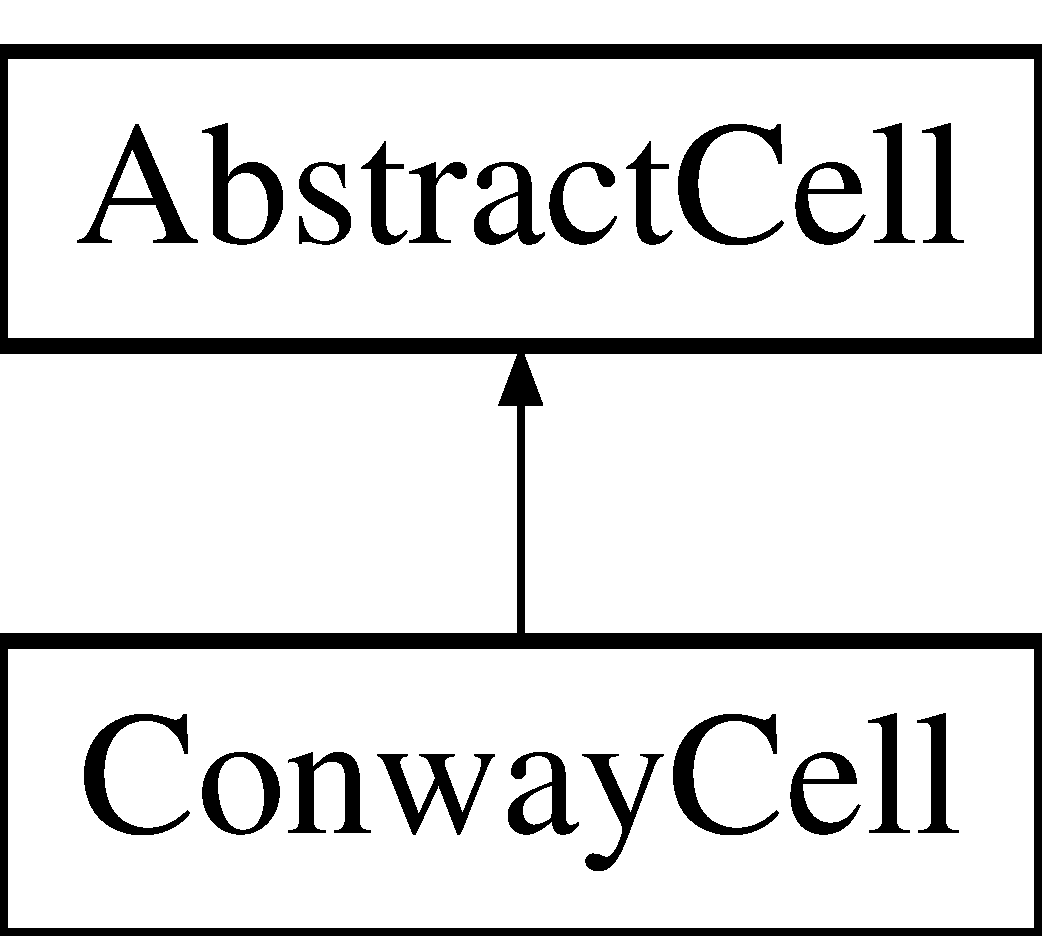
\includegraphics[height=2.000000cm]{classConwayCell}
\end{center}
\end{figure}
\subsection*{Public Member Functions}
\begin{DoxyCompactItemize}
\item 
\hyperlink{classConwayCell_aeff597ba7adcb28d4c386d075eddb196}{Conway\-Cell} ()
\item 
\hyperlink{classConwayCell_a62b809851f5cd9acfbc07d5a0ea283f1}{Conway\-Cell} (const \hyperlink{classConwayCell}{Conway\-Cell} \&)=default
\item 
\hyperlink{classConwayCell_a84ee85ecc83a697ae5954c24294a2af8}{Conway\-Cell} (\hyperlink{classConwayCell}{Conway\-Cell} \&\&)=default
\item 
\hyperlink{classConwayCell}{Conway\-Cell} \& \hyperlink{classConwayCell_aa83d009212f52ac55e39f42f002970a0}{operator=} (const \hyperlink{classConwayCell}{Conway\-Cell} \&)=default
\item 
\hyperlink{classConwayCell}{Conway\-Cell} \& \hyperlink{classConwayCell_a951cc1ac6d81cfea066a2076953fa209}{operator=} (\hyperlink{classConwayCell}{Conway\-Cell} \&\&)=default
\item 
\hyperlink{classConwayCell_a965899766787781cf4463ab080b56cb5}{$\sim$\-Conway\-Cell} ()=default
\item 
\hyperlink{classAbstractCell}{Abstract\-Cell} $\ast$ \hyperlink{classConwayCell_a00e3f8117929e7dcbb85f71aeaa10368}{clone} () const 
\item 
void \hyperlink{classConwayCell_a6a0d34c7f90a1b76e144c891ba4541e5}{update\-\_\-state} (string c)
\item 
int \hyperlink{classConwayCell_afbd79c8a5fc7a7da5885cdc7445f5b45}{count\-\_\-neighbor} (int possible\-\_\-nb\mbox{[}$\,$\mbox{]}) const 
\item 
string \hyperlink{classConwayCell_ad8be337992eca64445ebc1259af8d4ca}{print} ()
\item 
void \hyperlink{classConwayCell_a94a403a65aac5b0c9fd69c175122151c}{evolve} (int num\-\_\-neighbors)
\item 
int \hyperlink{classConwayCell_a49c7cf05666f19c89e8a0b29a78a6d3f}{cnt} ()
\item 
bool \hyperlink{classConwayCell_a5f0061fad24ab7d11c315f3e2dfe45be}{operator==} (const \hyperlink{classConwayCell}{Conway\-Cell} \&rhs) const 
\item 
\hyperlink{classConwayCell_a2067446abf91a0e431cfbfcef78655e9}{F\-R\-I\-E\-N\-D\-\_\-\-T\-E\-S\-T} (\hyperlink{classConwayCell_aaf9203db9ae10bf69d131c17aa7bf43c}{Conway\-Cell\-Test}, Conway\-Cell\-\_\-1)
\item 
\hyperlink{classConwayCell_aa53ff60436e507934569ad56ef9173e3}{F\-R\-I\-E\-N\-D\-\_\-\-T\-E\-S\-T} (\hyperlink{classConwayCell_aaf9203db9ae10bf69d131c17aa7bf43c}{Conway\-Cell\-Test}, Conway\-Cell\-\_\-2)
\item 
\hyperlink{classConwayCell_ad6c71e5f6e6d522ceac4238841840f19}{F\-R\-I\-E\-N\-D\-\_\-\-T\-E\-S\-T} (\hyperlink{classConwayCell_aaf9203db9ae10bf69d131c17aa7bf43c}{Conway\-Cell\-Test}, Conway\-Cell\-\_\-3)
\item 
\hyperlink{classConwayCell_a69db8d9316954fdf1743c6a71bc982c4}{F\-R\-I\-E\-N\-D\-\_\-\-T\-E\-S\-T} (\hyperlink{classConwayCell_aaf9203db9ae10bf69d131c17aa7bf43c}{Conway\-Cell\-Test}, clone\-\_\-1)
\item 
\hyperlink{classConwayCell_a3ab2d2c90bb57a8b50442b6100f0308c}{F\-R\-I\-E\-N\-D\-\_\-\-T\-E\-S\-T} (\hyperlink{classConwayCell_aaf9203db9ae10bf69d131c17aa7bf43c}{Conway\-Cell\-Test}, clone\-\_\-2)
\item 
\hyperlink{classConwayCell_aee7a7ab257ea971be8d495686919e571}{F\-R\-I\-E\-N\-D\-\_\-\-T\-E\-S\-T} (\hyperlink{classConwayCell_aaf9203db9ae10bf69d131c17aa7bf43c}{Conway\-Cell\-Test}, clone\-\_\-3)
\item 
\hyperlink{classConwayCell_ab8149e7169ca80bc99322e205fdc32d8}{F\-R\-I\-E\-N\-D\-\_\-\-T\-E\-S\-T} (\hyperlink{classConwayCell_aaf9203db9ae10bf69d131c17aa7bf43c}{Conway\-Cell\-Test}, update\-\_\-state\-\_\-1)
\item 
\hyperlink{classConwayCell_a69cf21e56a52a165b356afeaab25ed04}{F\-R\-I\-E\-N\-D\-\_\-\-T\-E\-S\-T} (\hyperlink{classConwayCell_aaf9203db9ae10bf69d131c17aa7bf43c}{Conway\-Cell\-Test}, update\-\_\-state\-\_\-2)
\item 
\hyperlink{classConwayCell_a99bd220d17a2e3690de9cf5e089f35cc}{F\-R\-I\-E\-N\-D\-\_\-\-T\-E\-S\-T} (\hyperlink{classConwayCell_aaf9203db9ae10bf69d131c17aa7bf43c}{Conway\-Cell\-Test}, update\-\_\-state\-\_\-3)
\item 
\hyperlink{classConwayCell_a0cc28543775075f67a5fde349eccfcbe}{F\-R\-I\-E\-N\-D\-\_\-\-T\-E\-S\-T} (\hyperlink{classConwayCell_aaf9203db9ae10bf69d131c17aa7bf43c}{Conway\-Cell\-Test}, count\-\_\-neighbor\-\_\-1)
\item 
\hyperlink{classConwayCell_af0c4905fac30c9919443297577ad7596}{F\-R\-I\-E\-N\-D\-\_\-\-T\-E\-S\-T} (\hyperlink{classConwayCell_aaf9203db9ae10bf69d131c17aa7bf43c}{Conway\-Cell\-Test}, count\-\_\-neighbor\-\_\-2)
\item 
\hyperlink{classConwayCell_a5d773d33e9e45dec53ff3e2695cfa2d1}{F\-R\-I\-E\-N\-D\-\_\-\-T\-E\-S\-T} (\hyperlink{classConwayCell_aaf9203db9ae10bf69d131c17aa7bf43c}{Conway\-Cell\-Test}, count\-\_\-neighbor\-\_\-3)
\item 
\hyperlink{classConwayCell_a2bb98a624065715ba41f16d10b6e9940}{F\-R\-I\-E\-N\-D\-\_\-\-T\-E\-S\-T} (\hyperlink{classConwayCell_aaf9203db9ae10bf69d131c17aa7bf43c}{Conway\-Cell\-Test}, print\-\_\-1)
\item 
\hyperlink{classConwayCell_a7242e24d1d1ef00e33e4c7a1c086402d}{F\-R\-I\-E\-N\-D\-\_\-\-T\-E\-S\-T} (\hyperlink{classConwayCell_aaf9203db9ae10bf69d131c17aa7bf43c}{Conway\-Cell\-Test}, print\-\_\-2)
\item 
\hyperlink{classConwayCell_aee2276a5977cdc6d699ac17461a3e695}{F\-R\-I\-E\-N\-D\-\_\-\-T\-E\-S\-T} (\hyperlink{classConwayCell_aaf9203db9ae10bf69d131c17aa7bf43c}{Conway\-Cell\-Test}, print\-\_\-3)
\item 
\hyperlink{classConwayCell_a5ec1d3543e64c91e7f5a4c102de94bd6}{F\-R\-I\-E\-N\-D\-\_\-\-T\-E\-S\-T} (\hyperlink{classConwayCell_aaf9203db9ae10bf69d131c17aa7bf43c}{Conway\-Cell\-Test}, evolve\-\_\-1)
\item 
\hyperlink{classConwayCell_a5c8705818153b330a7ec627abe35d1e2}{F\-R\-I\-E\-N\-D\-\_\-\-T\-E\-S\-T} (\hyperlink{classConwayCell_aaf9203db9ae10bf69d131c17aa7bf43c}{Conway\-Cell\-Test}, evolve\-\_\-2)
\item 
\hyperlink{classConwayCell_afe554afb102b15f42819bc5021d80dae}{F\-R\-I\-E\-N\-D\-\_\-\-T\-E\-S\-T} (\hyperlink{classConwayCell_aaf9203db9ae10bf69d131c17aa7bf43c}{Conway\-Cell\-Test}, evolve\-\_\-3)
\item 
\hyperlink{classConwayCell_acff342e1a23dad421d012916272d51f4}{F\-R\-I\-E\-N\-D\-\_\-\-T\-E\-S\-T} (\hyperlink{classConwayCell_aaf9203db9ae10bf69d131c17aa7bf43c}{Conway\-Cell\-Test}, cnt\-\_\-1)
\item 
\hyperlink{classConwayCell_add103ae6493c6aab58eeb8549c9c6aba}{F\-R\-I\-E\-N\-D\-\_\-\-T\-E\-S\-T} (\hyperlink{classConwayCell_aaf9203db9ae10bf69d131c17aa7bf43c}{Conway\-Cell\-Test}, cnt\-\_\-2)
\item 
\hyperlink{classConwayCell_a5cb196006329cfa5bb92b682297bddfa}{F\-R\-I\-E\-N\-D\-\_\-\-T\-E\-S\-T} (\hyperlink{classConwayCell_aaf9203db9ae10bf69d131c17aa7bf43c}{Conway\-Cell\-Test}, cnt\-\_\-3)
\item 
\hyperlink{classConwayCell_a5bb511ca635edd0de76fc7d7603b9617}{F\-R\-I\-E\-N\-D\-\_\-\-T\-E\-S\-T} (\hyperlink{classConwayCell_aaf9203db9ae10bf69d131c17aa7bf43c}{Conway\-Cell\-Test}, operator\-\_\-equal\-\_\-equal\-\_\-1)
\item 
\hyperlink{classConwayCell_abd78212cc3404f77b5a08f0686c190bd}{F\-R\-I\-E\-N\-D\-\_\-\-T\-E\-S\-T} (\hyperlink{classConwayCell_aaf9203db9ae10bf69d131c17aa7bf43c}{Conway\-Cell\-Test}, operator\-\_\-equal\-\_\-equal\-\_\-2)
\item 
\hyperlink{classConwayCell_a46f5c85b64001dedaaa8d859be53ebcf}{F\-R\-I\-E\-N\-D\-\_\-\-T\-E\-S\-T} (\hyperlink{classConwayCell_aaf9203db9ae10bf69d131c17aa7bf43c}{Conway\-Cell\-Test}, operator\-\_\-equal\-\_\-equal\-\_\-3)
\end{DoxyCompactItemize}
\subsection*{Friends}
\begin{DoxyCompactItemize}
\item 
class \hyperlink{classConwayCell_aaf9203db9ae10bf69d131c17aa7bf43c}{Conway\-Cell\-Test}
\end{DoxyCompactItemize}
\subsection*{Additional Inherited Members}


\subsection{Constructor \& Destructor Documentation}
\hypertarget{classConwayCell_aeff597ba7adcb28d4c386d075eddb196}{\index{Conway\-Cell@{Conway\-Cell}!Conway\-Cell@{Conway\-Cell}}
\index{Conway\-Cell@{Conway\-Cell}!ConwayCell@{Conway\-Cell}}
\subsubsection[{Conway\-Cell}]{\setlength{\rightskip}{0pt plus 5cm}Conway\-Cell\-::\-Conway\-Cell (
\begin{DoxyParamCaption}
{}
\end{DoxyParamCaption}
)}}\label{classConwayCell_aeff597ba7adcb28d4c386d075eddb196}

\begin{DoxyParams}{Parameters}
{\em String} & name and default \\
\hline
\end{DoxyParams}
\hypertarget{classConwayCell_a62b809851f5cd9acfbc07d5a0ea283f1}{\index{Conway\-Cell@{Conway\-Cell}!Conway\-Cell@{Conway\-Cell}}
\index{Conway\-Cell@{Conway\-Cell}!ConwayCell@{Conway\-Cell}}
\subsubsection[{Conway\-Cell}]{\setlength{\rightskip}{0pt plus 5cm}Conway\-Cell\-::\-Conway\-Cell (
\begin{DoxyParamCaption}
\item[{const {\bf Conway\-Cell} \&}]{}
\end{DoxyParamCaption}
)\hspace{0.3cm}{\ttfamily [default]}}}\label{classConwayCell_a62b809851f5cd9acfbc07d5a0ea283f1}
\hypertarget{classConwayCell_a84ee85ecc83a697ae5954c24294a2af8}{\index{Conway\-Cell@{Conway\-Cell}!Conway\-Cell@{Conway\-Cell}}
\index{Conway\-Cell@{Conway\-Cell}!ConwayCell@{Conway\-Cell}}
\subsubsection[{Conway\-Cell}]{\setlength{\rightskip}{0pt plus 5cm}Conway\-Cell\-::\-Conway\-Cell (
\begin{DoxyParamCaption}
\item[{{\bf Conway\-Cell} \&\&}]{}
\end{DoxyParamCaption}
)\hspace{0.3cm}{\ttfamily [default]}}}\label{classConwayCell_a84ee85ecc83a697ae5954c24294a2af8}
\hypertarget{classConwayCell_a965899766787781cf4463ab080b56cb5}{\index{Conway\-Cell@{Conway\-Cell}!$\sim$\-Conway\-Cell@{$\sim$\-Conway\-Cell}}
\index{$\sim$\-Conway\-Cell@{$\sim$\-Conway\-Cell}!ConwayCell@{Conway\-Cell}}
\subsubsection[{$\sim$\-Conway\-Cell}]{\setlength{\rightskip}{0pt plus 5cm}Conway\-Cell\-::$\sim$\-Conway\-Cell (
\begin{DoxyParamCaption}
{}
\end{DoxyParamCaption}
)\hspace{0.3cm}{\ttfamily [default]}}}\label{classConwayCell_a965899766787781cf4463ab080b56cb5}


\subsection{Member Function Documentation}
\hypertarget{classConwayCell_a00e3f8117929e7dcbb85f71aeaa10368}{\index{Conway\-Cell@{Conway\-Cell}!clone@{clone}}
\index{clone@{clone}!ConwayCell@{Conway\-Cell}}
\subsubsection[{clone}]{\setlength{\rightskip}{0pt plus 5cm}{\bf Abstract\-Cell} $\ast$ Conway\-Cell\-::clone (
\begin{DoxyParamCaption}
{}
\end{DoxyParamCaption}
) const\hspace{0.3cm}{\ttfamily [virtual]}}}\label{classConwayCell_a00e3f8117929e7dcbb85f71aeaa10368}


Implements \hyperlink{classAbstractCell_a1a95a7ea92b3503e2f042170b6320354}{Abstract\-Cell}.

\hypertarget{classConwayCell_a49c7cf05666f19c89e8a0b29a78a6d3f}{\index{Conway\-Cell@{Conway\-Cell}!cnt@{cnt}}
\index{cnt@{cnt}!ConwayCell@{Conway\-Cell}}
\subsubsection[{cnt}]{\setlength{\rightskip}{0pt plus 5cm}int Conway\-Cell\-::cnt (
\begin{DoxyParamCaption}
{}
\end{DoxyParamCaption}
)\hspace{0.3cm}{\ttfamily [virtual]}}}\label{classConwayCell_a49c7cf05666f19c89e8a0b29a78a6d3f}
\begin{DoxyReturn}{Returns}
count 1 for alived, count 0 for dead 
\end{DoxyReturn}


Implements \hyperlink{classAbstractCell_aac03c6e21580569ae306909e68feae9d}{Abstract\-Cell}.

\hypertarget{classConwayCell_afbd79c8a5fc7a7da5885cdc7445f5b45}{\index{Conway\-Cell@{Conway\-Cell}!count\-\_\-neighbor@{count\-\_\-neighbor}}
\index{count\-\_\-neighbor@{count\-\_\-neighbor}!ConwayCell@{Conway\-Cell}}
\subsubsection[{count\-\_\-neighbor}]{\setlength{\rightskip}{0pt plus 5cm}int Conway\-Cell\-::count\-\_\-neighbor (
\begin{DoxyParamCaption}
\item[{int}]{possible\-\_\-nb\mbox{[}$\,$\mbox{]}}
\end{DoxyParamCaption}
) const\hspace{0.3cm}{\ttfamily [virtual]}}}\label{classConwayCell_afbd79c8a5fc7a7da5885cdc7445f5b45}

\begin{DoxyParams}{Parameters}
{\em int\mbox{[}$\,$\mbox{]}} & of possible neighbors upto 8 neighbors \\
\hline
\end{DoxyParams}
\begin{DoxyReturn}{Returns}
int number of neighbor 
\end{DoxyReturn}


Implements \hyperlink{classAbstractCell_af566abaafe33b73bae0874566a987b63}{Abstract\-Cell}.

\hypertarget{classConwayCell_a94a403a65aac5b0c9fd69c175122151c}{\index{Conway\-Cell@{Conway\-Cell}!evolve@{evolve}}
\index{evolve@{evolve}!ConwayCell@{Conway\-Cell}}
\subsubsection[{evolve}]{\setlength{\rightskip}{0pt plus 5cm}void Conway\-Cell\-::evolve (
\begin{DoxyParamCaption}
\item[{int}]{num\-\_\-neighbors}
\end{DoxyParamCaption}
)\hspace{0.3cm}{\ttfamily [virtual]}}}\label{classConwayCell_a94a403a65aac5b0c9fd69c175122151c}

\begin{DoxyParams}{Parameters}
{\em int} & number of neighbors \\
\hline
\end{DoxyParams}


Implements \hyperlink{classAbstractCell_ad46c73f9a67419ecd570a7677525054f}{Abstract\-Cell}.

\hypertarget{classConwayCell_a2067446abf91a0e431cfbfcef78655e9}{\index{Conway\-Cell@{Conway\-Cell}!F\-R\-I\-E\-N\-D\-\_\-\-T\-E\-S\-T@{F\-R\-I\-E\-N\-D\-\_\-\-T\-E\-S\-T}}
\index{F\-R\-I\-E\-N\-D\-\_\-\-T\-E\-S\-T@{F\-R\-I\-E\-N\-D\-\_\-\-T\-E\-S\-T}!ConwayCell@{Conway\-Cell}}
\subsubsection[{F\-R\-I\-E\-N\-D\-\_\-\-T\-E\-S\-T}]{\setlength{\rightskip}{0pt plus 5cm}Conway\-Cell\-::\-F\-R\-I\-E\-N\-D\-\_\-\-T\-E\-S\-T (
\begin{DoxyParamCaption}
\item[{{\bf Conway\-Cell\-Test}}]{, }
\item[{Conway\-Cell\-\_\-1}]{}
\end{DoxyParamCaption}
)}}\label{classConwayCell_a2067446abf91a0e431cfbfcef78655e9}
\hypertarget{classConwayCell_aa53ff60436e507934569ad56ef9173e3}{\index{Conway\-Cell@{Conway\-Cell}!F\-R\-I\-E\-N\-D\-\_\-\-T\-E\-S\-T@{F\-R\-I\-E\-N\-D\-\_\-\-T\-E\-S\-T}}
\index{F\-R\-I\-E\-N\-D\-\_\-\-T\-E\-S\-T@{F\-R\-I\-E\-N\-D\-\_\-\-T\-E\-S\-T}!ConwayCell@{Conway\-Cell}}
\subsubsection[{F\-R\-I\-E\-N\-D\-\_\-\-T\-E\-S\-T}]{\setlength{\rightskip}{0pt plus 5cm}Conway\-Cell\-::\-F\-R\-I\-E\-N\-D\-\_\-\-T\-E\-S\-T (
\begin{DoxyParamCaption}
\item[{{\bf Conway\-Cell\-Test}}]{, }
\item[{Conway\-Cell\-\_\-2}]{}
\end{DoxyParamCaption}
)}}\label{classConwayCell_aa53ff60436e507934569ad56ef9173e3}
\hypertarget{classConwayCell_ad6c71e5f6e6d522ceac4238841840f19}{\index{Conway\-Cell@{Conway\-Cell}!F\-R\-I\-E\-N\-D\-\_\-\-T\-E\-S\-T@{F\-R\-I\-E\-N\-D\-\_\-\-T\-E\-S\-T}}
\index{F\-R\-I\-E\-N\-D\-\_\-\-T\-E\-S\-T@{F\-R\-I\-E\-N\-D\-\_\-\-T\-E\-S\-T}!ConwayCell@{Conway\-Cell}}
\subsubsection[{F\-R\-I\-E\-N\-D\-\_\-\-T\-E\-S\-T}]{\setlength{\rightskip}{0pt plus 5cm}Conway\-Cell\-::\-F\-R\-I\-E\-N\-D\-\_\-\-T\-E\-S\-T (
\begin{DoxyParamCaption}
\item[{{\bf Conway\-Cell\-Test}}]{, }
\item[{Conway\-Cell\-\_\-3}]{}
\end{DoxyParamCaption}
)}}\label{classConwayCell_ad6c71e5f6e6d522ceac4238841840f19}
\hypertarget{classConwayCell_a69db8d9316954fdf1743c6a71bc982c4}{\index{Conway\-Cell@{Conway\-Cell}!F\-R\-I\-E\-N\-D\-\_\-\-T\-E\-S\-T@{F\-R\-I\-E\-N\-D\-\_\-\-T\-E\-S\-T}}
\index{F\-R\-I\-E\-N\-D\-\_\-\-T\-E\-S\-T@{F\-R\-I\-E\-N\-D\-\_\-\-T\-E\-S\-T}!ConwayCell@{Conway\-Cell}}
\subsubsection[{F\-R\-I\-E\-N\-D\-\_\-\-T\-E\-S\-T}]{\setlength{\rightskip}{0pt plus 5cm}Conway\-Cell\-::\-F\-R\-I\-E\-N\-D\-\_\-\-T\-E\-S\-T (
\begin{DoxyParamCaption}
\item[{{\bf Conway\-Cell\-Test}}]{, }
\item[{clone\-\_\-1}]{}
\end{DoxyParamCaption}
)}}\label{classConwayCell_a69db8d9316954fdf1743c6a71bc982c4}
\hypertarget{classConwayCell_a3ab2d2c90bb57a8b50442b6100f0308c}{\index{Conway\-Cell@{Conway\-Cell}!F\-R\-I\-E\-N\-D\-\_\-\-T\-E\-S\-T@{F\-R\-I\-E\-N\-D\-\_\-\-T\-E\-S\-T}}
\index{F\-R\-I\-E\-N\-D\-\_\-\-T\-E\-S\-T@{F\-R\-I\-E\-N\-D\-\_\-\-T\-E\-S\-T}!ConwayCell@{Conway\-Cell}}
\subsubsection[{F\-R\-I\-E\-N\-D\-\_\-\-T\-E\-S\-T}]{\setlength{\rightskip}{0pt plus 5cm}Conway\-Cell\-::\-F\-R\-I\-E\-N\-D\-\_\-\-T\-E\-S\-T (
\begin{DoxyParamCaption}
\item[{{\bf Conway\-Cell\-Test}}]{, }
\item[{clone\-\_\-2}]{}
\end{DoxyParamCaption}
)}}\label{classConwayCell_a3ab2d2c90bb57a8b50442b6100f0308c}
\hypertarget{classConwayCell_aee7a7ab257ea971be8d495686919e571}{\index{Conway\-Cell@{Conway\-Cell}!F\-R\-I\-E\-N\-D\-\_\-\-T\-E\-S\-T@{F\-R\-I\-E\-N\-D\-\_\-\-T\-E\-S\-T}}
\index{F\-R\-I\-E\-N\-D\-\_\-\-T\-E\-S\-T@{F\-R\-I\-E\-N\-D\-\_\-\-T\-E\-S\-T}!ConwayCell@{Conway\-Cell}}
\subsubsection[{F\-R\-I\-E\-N\-D\-\_\-\-T\-E\-S\-T}]{\setlength{\rightskip}{0pt plus 5cm}Conway\-Cell\-::\-F\-R\-I\-E\-N\-D\-\_\-\-T\-E\-S\-T (
\begin{DoxyParamCaption}
\item[{{\bf Conway\-Cell\-Test}}]{, }
\item[{clone\-\_\-3}]{}
\end{DoxyParamCaption}
)}}\label{classConwayCell_aee7a7ab257ea971be8d495686919e571}
\hypertarget{classConwayCell_ab8149e7169ca80bc99322e205fdc32d8}{\index{Conway\-Cell@{Conway\-Cell}!F\-R\-I\-E\-N\-D\-\_\-\-T\-E\-S\-T@{F\-R\-I\-E\-N\-D\-\_\-\-T\-E\-S\-T}}
\index{F\-R\-I\-E\-N\-D\-\_\-\-T\-E\-S\-T@{F\-R\-I\-E\-N\-D\-\_\-\-T\-E\-S\-T}!ConwayCell@{Conway\-Cell}}
\subsubsection[{F\-R\-I\-E\-N\-D\-\_\-\-T\-E\-S\-T}]{\setlength{\rightskip}{0pt plus 5cm}Conway\-Cell\-::\-F\-R\-I\-E\-N\-D\-\_\-\-T\-E\-S\-T (
\begin{DoxyParamCaption}
\item[{{\bf Conway\-Cell\-Test}}]{, }
\item[{update\-\_\-state\-\_\-1}]{}
\end{DoxyParamCaption}
)}}\label{classConwayCell_ab8149e7169ca80bc99322e205fdc32d8}
\hypertarget{classConwayCell_a69cf21e56a52a165b356afeaab25ed04}{\index{Conway\-Cell@{Conway\-Cell}!F\-R\-I\-E\-N\-D\-\_\-\-T\-E\-S\-T@{F\-R\-I\-E\-N\-D\-\_\-\-T\-E\-S\-T}}
\index{F\-R\-I\-E\-N\-D\-\_\-\-T\-E\-S\-T@{F\-R\-I\-E\-N\-D\-\_\-\-T\-E\-S\-T}!ConwayCell@{Conway\-Cell}}
\subsubsection[{F\-R\-I\-E\-N\-D\-\_\-\-T\-E\-S\-T}]{\setlength{\rightskip}{0pt plus 5cm}Conway\-Cell\-::\-F\-R\-I\-E\-N\-D\-\_\-\-T\-E\-S\-T (
\begin{DoxyParamCaption}
\item[{{\bf Conway\-Cell\-Test}}]{, }
\item[{update\-\_\-state\-\_\-2}]{}
\end{DoxyParamCaption}
)}}\label{classConwayCell_a69cf21e56a52a165b356afeaab25ed04}
\hypertarget{classConwayCell_a99bd220d17a2e3690de9cf5e089f35cc}{\index{Conway\-Cell@{Conway\-Cell}!F\-R\-I\-E\-N\-D\-\_\-\-T\-E\-S\-T@{F\-R\-I\-E\-N\-D\-\_\-\-T\-E\-S\-T}}
\index{F\-R\-I\-E\-N\-D\-\_\-\-T\-E\-S\-T@{F\-R\-I\-E\-N\-D\-\_\-\-T\-E\-S\-T}!ConwayCell@{Conway\-Cell}}
\subsubsection[{F\-R\-I\-E\-N\-D\-\_\-\-T\-E\-S\-T}]{\setlength{\rightskip}{0pt plus 5cm}Conway\-Cell\-::\-F\-R\-I\-E\-N\-D\-\_\-\-T\-E\-S\-T (
\begin{DoxyParamCaption}
\item[{{\bf Conway\-Cell\-Test}}]{, }
\item[{update\-\_\-state\-\_\-3}]{}
\end{DoxyParamCaption}
)}}\label{classConwayCell_a99bd220d17a2e3690de9cf5e089f35cc}
\hypertarget{classConwayCell_a0cc28543775075f67a5fde349eccfcbe}{\index{Conway\-Cell@{Conway\-Cell}!F\-R\-I\-E\-N\-D\-\_\-\-T\-E\-S\-T@{F\-R\-I\-E\-N\-D\-\_\-\-T\-E\-S\-T}}
\index{F\-R\-I\-E\-N\-D\-\_\-\-T\-E\-S\-T@{F\-R\-I\-E\-N\-D\-\_\-\-T\-E\-S\-T}!ConwayCell@{Conway\-Cell}}
\subsubsection[{F\-R\-I\-E\-N\-D\-\_\-\-T\-E\-S\-T}]{\setlength{\rightskip}{0pt plus 5cm}Conway\-Cell\-::\-F\-R\-I\-E\-N\-D\-\_\-\-T\-E\-S\-T (
\begin{DoxyParamCaption}
\item[{{\bf Conway\-Cell\-Test}}]{, }
\item[{count\-\_\-neighbor\-\_\-1}]{}
\end{DoxyParamCaption}
)}}\label{classConwayCell_a0cc28543775075f67a5fde349eccfcbe}
\hypertarget{classConwayCell_af0c4905fac30c9919443297577ad7596}{\index{Conway\-Cell@{Conway\-Cell}!F\-R\-I\-E\-N\-D\-\_\-\-T\-E\-S\-T@{F\-R\-I\-E\-N\-D\-\_\-\-T\-E\-S\-T}}
\index{F\-R\-I\-E\-N\-D\-\_\-\-T\-E\-S\-T@{F\-R\-I\-E\-N\-D\-\_\-\-T\-E\-S\-T}!ConwayCell@{Conway\-Cell}}
\subsubsection[{F\-R\-I\-E\-N\-D\-\_\-\-T\-E\-S\-T}]{\setlength{\rightskip}{0pt plus 5cm}Conway\-Cell\-::\-F\-R\-I\-E\-N\-D\-\_\-\-T\-E\-S\-T (
\begin{DoxyParamCaption}
\item[{{\bf Conway\-Cell\-Test}}]{, }
\item[{count\-\_\-neighbor\-\_\-2}]{}
\end{DoxyParamCaption}
)}}\label{classConwayCell_af0c4905fac30c9919443297577ad7596}
\hypertarget{classConwayCell_a5d773d33e9e45dec53ff3e2695cfa2d1}{\index{Conway\-Cell@{Conway\-Cell}!F\-R\-I\-E\-N\-D\-\_\-\-T\-E\-S\-T@{F\-R\-I\-E\-N\-D\-\_\-\-T\-E\-S\-T}}
\index{F\-R\-I\-E\-N\-D\-\_\-\-T\-E\-S\-T@{F\-R\-I\-E\-N\-D\-\_\-\-T\-E\-S\-T}!ConwayCell@{Conway\-Cell}}
\subsubsection[{F\-R\-I\-E\-N\-D\-\_\-\-T\-E\-S\-T}]{\setlength{\rightskip}{0pt plus 5cm}Conway\-Cell\-::\-F\-R\-I\-E\-N\-D\-\_\-\-T\-E\-S\-T (
\begin{DoxyParamCaption}
\item[{{\bf Conway\-Cell\-Test}}]{, }
\item[{count\-\_\-neighbor\-\_\-3}]{}
\end{DoxyParamCaption}
)}}\label{classConwayCell_a5d773d33e9e45dec53ff3e2695cfa2d1}
\hypertarget{classConwayCell_a2bb98a624065715ba41f16d10b6e9940}{\index{Conway\-Cell@{Conway\-Cell}!F\-R\-I\-E\-N\-D\-\_\-\-T\-E\-S\-T@{F\-R\-I\-E\-N\-D\-\_\-\-T\-E\-S\-T}}
\index{F\-R\-I\-E\-N\-D\-\_\-\-T\-E\-S\-T@{F\-R\-I\-E\-N\-D\-\_\-\-T\-E\-S\-T}!ConwayCell@{Conway\-Cell}}
\subsubsection[{F\-R\-I\-E\-N\-D\-\_\-\-T\-E\-S\-T}]{\setlength{\rightskip}{0pt plus 5cm}Conway\-Cell\-::\-F\-R\-I\-E\-N\-D\-\_\-\-T\-E\-S\-T (
\begin{DoxyParamCaption}
\item[{{\bf Conway\-Cell\-Test}}]{, }
\item[{print\-\_\-1}]{}
\end{DoxyParamCaption}
)}}\label{classConwayCell_a2bb98a624065715ba41f16d10b6e9940}
\hypertarget{classConwayCell_a7242e24d1d1ef00e33e4c7a1c086402d}{\index{Conway\-Cell@{Conway\-Cell}!F\-R\-I\-E\-N\-D\-\_\-\-T\-E\-S\-T@{F\-R\-I\-E\-N\-D\-\_\-\-T\-E\-S\-T}}
\index{F\-R\-I\-E\-N\-D\-\_\-\-T\-E\-S\-T@{F\-R\-I\-E\-N\-D\-\_\-\-T\-E\-S\-T}!ConwayCell@{Conway\-Cell}}
\subsubsection[{F\-R\-I\-E\-N\-D\-\_\-\-T\-E\-S\-T}]{\setlength{\rightskip}{0pt plus 5cm}Conway\-Cell\-::\-F\-R\-I\-E\-N\-D\-\_\-\-T\-E\-S\-T (
\begin{DoxyParamCaption}
\item[{{\bf Conway\-Cell\-Test}}]{, }
\item[{print\-\_\-2}]{}
\end{DoxyParamCaption}
)}}\label{classConwayCell_a7242e24d1d1ef00e33e4c7a1c086402d}
\hypertarget{classConwayCell_aee2276a5977cdc6d699ac17461a3e695}{\index{Conway\-Cell@{Conway\-Cell}!F\-R\-I\-E\-N\-D\-\_\-\-T\-E\-S\-T@{F\-R\-I\-E\-N\-D\-\_\-\-T\-E\-S\-T}}
\index{F\-R\-I\-E\-N\-D\-\_\-\-T\-E\-S\-T@{F\-R\-I\-E\-N\-D\-\_\-\-T\-E\-S\-T}!ConwayCell@{Conway\-Cell}}
\subsubsection[{F\-R\-I\-E\-N\-D\-\_\-\-T\-E\-S\-T}]{\setlength{\rightskip}{0pt plus 5cm}Conway\-Cell\-::\-F\-R\-I\-E\-N\-D\-\_\-\-T\-E\-S\-T (
\begin{DoxyParamCaption}
\item[{{\bf Conway\-Cell\-Test}}]{, }
\item[{print\-\_\-3}]{}
\end{DoxyParamCaption}
)}}\label{classConwayCell_aee2276a5977cdc6d699ac17461a3e695}
\hypertarget{classConwayCell_a5ec1d3543e64c91e7f5a4c102de94bd6}{\index{Conway\-Cell@{Conway\-Cell}!F\-R\-I\-E\-N\-D\-\_\-\-T\-E\-S\-T@{F\-R\-I\-E\-N\-D\-\_\-\-T\-E\-S\-T}}
\index{F\-R\-I\-E\-N\-D\-\_\-\-T\-E\-S\-T@{F\-R\-I\-E\-N\-D\-\_\-\-T\-E\-S\-T}!ConwayCell@{Conway\-Cell}}
\subsubsection[{F\-R\-I\-E\-N\-D\-\_\-\-T\-E\-S\-T}]{\setlength{\rightskip}{0pt plus 5cm}Conway\-Cell\-::\-F\-R\-I\-E\-N\-D\-\_\-\-T\-E\-S\-T (
\begin{DoxyParamCaption}
\item[{{\bf Conway\-Cell\-Test}}]{, }
\item[{evolve\-\_\-1}]{}
\end{DoxyParamCaption}
)}}\label{classConwayCell_a5ec1d3543e64c91e7f5a4c102de94bd6}
\hypertarget{classConwayCell_a5c8705818153b330a7ec627abe35d1e2}{\index{Conway\-Cell@{Conway\-Cell}!F\-R\-I\-E\-N\-D\-\_\-\-T\-E\-S\-T@{F\-R\-I\-E\-N\-D\-\_\-\-T\-E\-S\-T}}
\index{F\-R\-I\-E\-N\-D\-\_\-\-T\-E\-S\-T@{F\-R\-I\-E\-N\-D\-\_\-\-T\-E\-S\-T}!ConwayCell@{Conway\-Cell}}
\subsubsection[{F\-R\-I\-E\-N\-D\-\_\-\-T\-E\-S\-T}]{\setlength{\rightskip}{0pt plus 5cm}Conway\-Cell\-::\-F\-R\-I\-E\-N\-D\-\_\-\-T\-E\-S\-T (
\begin{DoxyParamCaption}
\item[{{\bf Conway\-Cell\-Test}}]{, }
\item[{evolve\-\_\-2}]{}
\end{DoxyParamCaption}
)}}\label{classConwayCell_a5c8705818153b330a7ec627abe35d1e2}
\hypertarget{classConwayCell_afe554afb102b15f42819bc5021d80dae}{\index{Conway\-Cell@{Conway\-Cell}!F\-R\-I\-E\-N\-D\-\_\-\-T\-E\-S\-T@{F\-R\-I\-E\-N\-D\-\_\-\-T\-E\-S\-T}}
\index{F\-R\-I\-E\-N\-D\-\_\-\-T\-E\-S\-T@{F\-R\-I\-E\-N\-D\-\_\-\-T\-E\-S\-T}!ConwayCell@{Conway\-Cell}}
\subsubsection[{F\-R\-I\-E\-N\-D\-\_\-\-T\-E\-S\-T}]{\setlength{\rightskip}{0pt plus 5cm}Conway\-Cell\-::\-F\-R\-I\-E\-N\-D\-\_\-\-T\-E\-S\-T (
\begin{DoxyParamCaption}
\item[{{\bf Conway\-Cell\-Test}}]{, }
\item[{evolve\-\_\-3}]{}
\end{DoxyParamCaption}
)}}\label{classConwayCell_afe554afb102b15f42819bc5021d80dae}
\hypertarget{classConwayCell_acff342e1a23dad421d012916272d51f4}{\index{Conway\-Cell@{Conway\-Cell}!F\-R\-I\-E\-N\-D\-\_\-\-T\-E\-S\-T@{F\-R\-I\-E\-N\-D\-\_\-\-T\-E\-S\-T}}
\index{F\-R\-I\-E\-N\-D\-\_\-\-T\-E\-S\-T@{F\-R\-I\-E\-N\-D\-\_\-\-T\-E\-S\-T}!ConwayCell@{Conway\-Cell}}
\subsubsection[{F\-R\-I\-E\-N\-D\-\_\-\-T\-E\-S\-T}]{\setlength{\rightskip}{0pt plus 5cm}Conway\-Cell\-::\-F\-R\-I\-E\-N\-D\-\_\-\-T\-E\-S\-T (
\begin{DoxyParamCaption}
\item[{{\bf Conway\-Cell\-Test}}]{, }
\item[{cnt\-\_\-1}]{}
\end{DoxyParamCaption}
)}}\label{classConwayCell_acff342e1a23dad421d012916272d51f4}
\hypertarget{classConwayCell_add103ae6493c6aab58eeb8549c9c6aba}{\index{Conway\-Cell@{Conway\-Cell}!F\-R\-I\-E\-N\-D\-\_\-\-T\-E\-S\-T@{F\-R\-I\-E\-N\-D\-\_\-\-T\-E\-S\-T}}
\index{F\-R\-I\-E\-N\-D\-\_\-\-T\-E\-S\-T@{F\-R\-I\-E\-N\-D\-\_\-\-T\-E\-S\-T}!ConwayCell@{Conway\-Cell}}
\subsubsection[{F\-R\-I\-E\-N\-D\-\_\-\-T\-E\-S\-T}]{\setlength{\rightskip}{0pt plus 5cm}Conway\-Cell\-::\-F\-R\-I\-E\-N\-D\-\_\-\-T\-E\-S\-T (
\begin{DoxyParamCaption}
\item[{{\bf Conway\-Cell\-Test}}]{, }
\item[{cnt\-\_\-2}]{}
\end{DoxyParamCaption}
)}}\label{classConwayCell_add103ae6493c6aab58eeb8549c9c6aba}
\hypertarget{classConwayCell_a5cb196006329cfa5bb92b682297bddfa}{\index{Conway\-Cell@{Conway\-Cell}!F\-R\-I\-E\-N\-D\-\_\-\-T\-E\-S\-T@{F\-R\-I\-E\-N\-D\-\_\-\-T\-E\-S\-T}}
\index{F\-R\-I\-E\-N\-D\-\_\-\-T\-E\-S\-T@{F\-R\-I\-E\-N\-D\-\_\-\-T\-E\-S\-T}!ConwayCell@{Conway\-Cell}}
\subsubsection[{F\-R\-I\-E\-N\-D\-\_\-\-T\-E\-S\-T}]{\setlength{\rightskip}{0pt plus 5cm}Conway\-Cell\-::\-F\-R\-I\-E\-N\-D\-\_\-\-T\-E\-S\-T (
\begin{DoxyParamCaption}
\item[{{\bf Conway\-Cell\-Test}}]{, }
\item[{cnt\-\_\-3}]{}
\end{DoxyParamCaption}
)}}\label{classConwayCell_a5cb196006329cfa5bb92b682297bddfa}
\hypertarget{classConwayCell_a5bb511ca635edd0de76fc7d7603b9617}{\index{Conway\-Cell@{Conway\-Cell}!F\-R\-I\-E\-N\-D\-\_\-\-T\-E\-S\-T@{F\-R\-I\-E\-N\-D\-\_\-\-T\-E\-S\-T}}
\index{F\-R\-I\-E\-N\-D\-\_\-\-T\-E\-S\-T@{F\-R\-I\-E\-N\-D\-\_\-\-T\-E\-S\-T}!ConwayCell@{Conway\-Cell}}
\subsubsection[{F\-R\-I\-E\-N\-D\-\_\-\-T\-E\-S\-T}]{\setlength{\rightskip}{0pt plus 5cm}Conway\-Cell\-::\-F\-R\-I\-E\-N\-D\-\_\-\-T\-E\-S\-T (
\begin{DoxyParamCaption}
\item[{{\bf Conway\-Cell\-Test}}]{, }
\item[{operator\-\_\-equal\-\_\-equal\-\_\-1}]{}
\end{DoxyParamCaption}
)}}\label{classConwayCell_a5bb511ca635edd0de76fc7d7603b9617}
\hypertarget{classConwayCell_abd78212cc3404f77b5a08f0686c190bd}{\index{Conway\-Cell@{Conway\-Cell}!F\-R\-I\-E\-N\-D\-\_\-\-T\-E\-S\-T@{F\-R\-I\-E\-N\-D\-\_\-\-T\-E\-S\-T}}
\index{F\-R\-I\-E\-N\-D\-\_\-\-T\-E\-S\-T@{F\-R\-I\-E\-N\-D\-\_\-\-T\-E\-S\-T}!ConwayCell@{Conway\-Cell}}
\subsubsection[{F\-R\-I\-E\-N\-D\-\_\-\-T\-E\-S\-T}]{\setlength{\rightskip}{0pt plus 5cm}Conway\-Cell\-::\-F\-R\-I\-E\-N\-D\-\_\-\-T\-E\-S\-T (
\begin{DoxyParamCaption}
\item[{{\bf Conway\-Cell\-Test}}]{, }
\item[{operator\-\_\-equal\-\_\-equal\-\_\-2}]{}
\end{DoxyParamCaption}
)}}\label{classConwayCell_abd78212cc3404f77b5a08f0686c190bd}
\hypertarget{classConwayCell_a46f5c85b64001dedaaa8d859be53ebcf}{\index{Conway\-Cell@{Conway\-Cell}!F\-R\-I\-E\-N\-D\-\_\-\-T\-E\-S\-T@{F\-R\-I\-E\-N\-D\-\_\-\-T\-E\-S\-T}}
\index{F\-R\-I\-E\-N\-D\-\_\-\-T\-E\-S\-T@{F\-R\-I\-E\-N\-D\-\_\-\-T\-E\-S\-T}!ConwayCell@{Conway\-Cell}}
\subsubsection[{F\-R\-I\-E\-N\-D\-\_\-\-T\-E\-S\-T}]{\setlength{\rightskip}{0pt plus 5cm}Conway\-Cell\-::\-F\-R\-I\-E\-N\-D\-\_\-\-T\-E\-S\-T (
\begin{DoxyParamCaption}
\item[{{\bf Conway\-Cell\-Test}}]{, }
\item[{operator\-\_\-equal\-\_\-equal\-\_\-3}]{}
\end{DoxyParamCaption}
)}}\label{classConwayCell_a46f5c85b64001dedaaa8d859be53ebcf}
\hypertarget{classConwayCell_aa83d009212f52ac55e39f42f002970a0}{\index{Conway\-Cell@{Conway\-Cell}!operator=@{operator=}}
\index{operator=@{operator=}!ConwayCell@{Conway\-Cell}}
\subsubsection[{operator=}]{\setlength{\rightskip}{0pt plus 5cm}{\bf Conway\-Cell}\& Conway\-Cell\-::operator= (
\begin{DoxyParamCaption}
\item[{const {\bf Conway\-Cell} \&}]{}
\end{DoxyParamCaption}
)\hspace{0.3cm}{\ttfamily [default]}}}\label{classConwayCell_aa83d009212f52ac55e39f42f002970a0}
\hypertarget{classConwayCell_a951cc1ac6d81cfea066a2076953fa209}{\index{Conway\-Cell@{Conway\-Cell}!operator=@{operator=}}
\index{operator=@{operator=}!ConwayCell@{Conway\-Cell}}
\subsubsection[{operator=}]{\setlength{\rightskip}{0pt plus 5cm}{\bf Conway\-Cell}\& Conway\-Cell\-::operator= (
\begin{DoxyParamCaption}
\item[{{\bf Conway\-Cell} \&\&}]{}
\end{DoxyParamCaption}
)\hspace{0.3cm}{\ttfamily [default]}}}\label{classConwayCell_a951cc1ac6d81cfea066a2076953fa209}
\hypertarget{classConwayCell_a5f0061fad24ab7d11c315f3e2dfe45be}{\index{Conway\-Cell@{Conway\-Cell}!operator==@{operator==}}
\index{operator==@{operator==}!ConwayCell@{Conway\-Cell}}
\subsubsection[{operator==}]{\setlength{\rightskip}{0pt plus 5cm}bool Conway\-Cell\-::operator== (
\begin{DoxyParamCaption}
\item[{const {\bf Conway\-Cell} \&}]{rhs}
\end{DoxyParamCaption}
) const}}\label{classConwayCell_a5f0061fad24ab7d11c315f3e2dfe45be}

\begin{DoxyParams}{Parameters}
{\em other} & \hyperlink{classConwayCell}{Conway\-Cell} \\
\hline
\end{DoxyParams}
\begin{DoxyReturn}{Returns}
true for equal, otherwise false 
\end{DoxyReturn}
\hypertarget{classConwayCell_ad8be337992eca64445ebc1259af8d4ca}{\index{Conway\-Cell@{Conway\-Cell}!print@{print}}
\index{print@{print}!ConwayCell@{Conway\-Cell}}
\subsubsection[{print}]{\setlength{\rightskip}{0pt plus 5cm}string Conway\-Cell\-::print (
\begin{DoxyParamCaption}
{}
\end{DoxyParamCaption}
)\hspace{0.3cm}{\ttfamily [virtual]}}}\label{classConwayCell_ad8be337992eca64445ebc1259af8d4ca}

\begin{DoxyParams}{Parameters}
{\em @return} & string character of the cell state \\
\hline
\end{DoxyParams}


Implements \hyperlink{classAbstractCell_a63e875724c1ee0278449d9489211baa7}{Abstract\-Cell}.

\hypertarget{classConwayCell_a6a0d34c7f90a1b76e144c891ba4541e5}{\index{Conway\-Cell@{Conway\-Cell}!update\-\_\-state@{update\-\_\-state}}
\index{update\-\_\-state@{update\-\_\-state}!ConwayCell@{Conway\-Cell}}
\subsubsection[{update\-\_\-state}]{\setlength{\rightskip}{0pt plus 5cm}void Conway\-Cell\-::update\-\_\-state (
\begin{DoxyParamCaption}
\item[{string}]{c}
\end{DoxyParamCaption}
)\hspace{0.3cm}{\ttfamily [virtual]}}}\label{classConwayCell_a6a0d34c7f90a1b76e144c891ba4541e5}

\begin{DoxyParams}{Parameters}
{\em String} & character \\
\hline
\end{DoxyParams}


Implements \hyperlink{classAbstractCell_a67008aedffea84aac7088ec84e8441cc}{Abstract\-Cell}.



\subsection{Friends And Related Function Documentation}
\hypertarget{classConwayCell_aaf9203db9ae10bf69d131c17aa7bf43c}{\index{Conway\-Cell@{Conway\-Cell}!Conway\-Cell\-Test@{Conway\-Cell\-Test}}
\index{Conway\-Cell\-Test@{Conway\-Cell\-Test}!ConwayCell@{Conway\-Cell}}
\subsubsection[{Conway\-Cell\-Test}]{\setlength{\rightskip}{0pt plus 5cm}friend class Conway\-Cell\-Test\hspace{0.3cm}{\ttfamily [friend]}}}\label{classConwayCell_aaf9203db9ae10bf69d131c17aa7bf43c}


The documentation for this class was generated from the following files\-:\begin{DoxyCompactItemize}
\item 
\hyperlink{Life_8h}{Life.\-h}\item 
\hyperlink{Life_8c_09_09}{Life.\-c++}\end{DoxyCompactItemize}

\hypertarget{classFredkinCell}{\section{Fredkin\-Cell Class Reference}
\label{classFredkinCell}\index{Fredkin\-Cell@{Fredkin\-Cell}}
}


{\ttfamily \#include $<$Life.\-h$>$}

Inheritance diagram for Fredkin\-Cell\-:\begin{figure}[H]
\begin{center}
\leavevmode
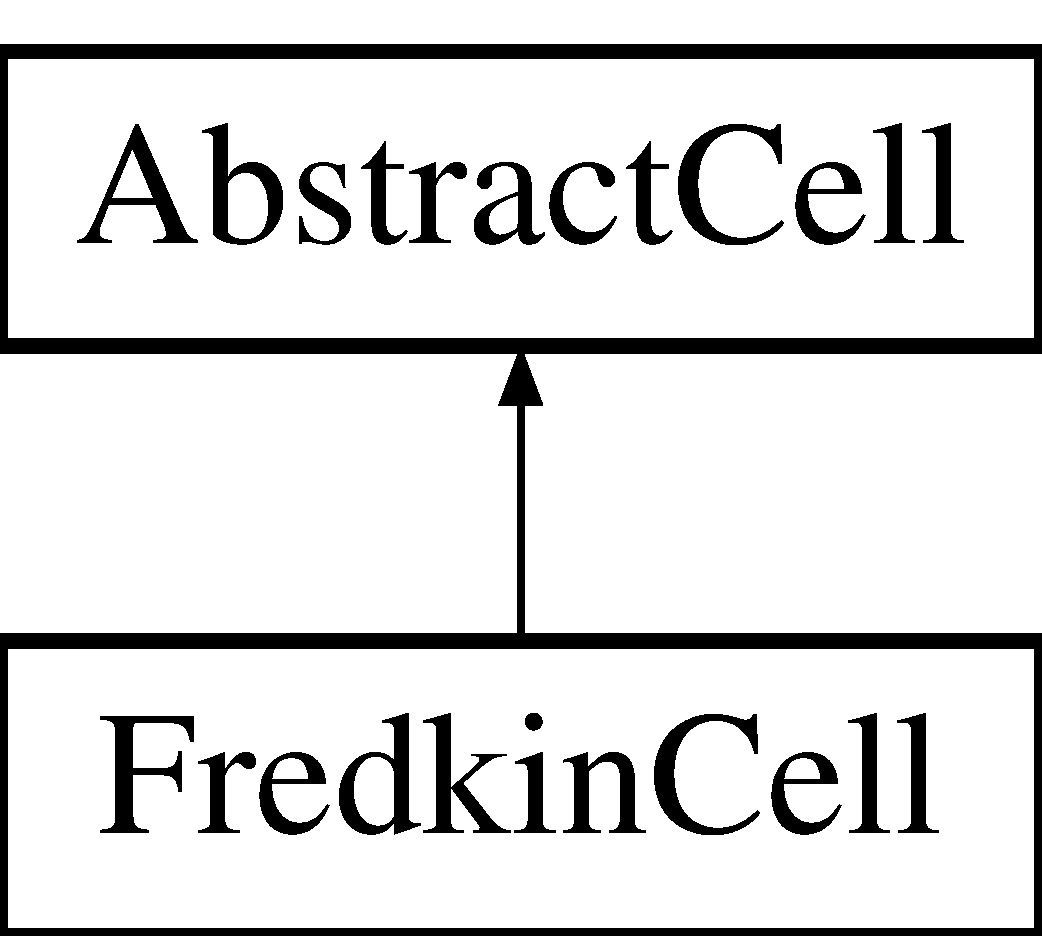
\includegraphics[height=2.000000cm]{classFredkinCell}
\end{center}
\end{figure}
\subsection*{Public Member Functions}
\begin{DoxyCompactItemize}
\item 
\hyperlink{classFredkinCell_ac5bd5726da496a3b3363d9c1b57dccc2}{Fredkin\-Cell} ()
\item 
\hyperlink{classFredkinCell_aa2c87b549c4010b0e9197fdc66a8e370}{Fredkin\-Cell} (const \hyperlink{classFredkinCell}{Fredkin\-Cell} \&)=default
\item 
\hyperlink{classFredkinCell_a0599a144fd1da99eb3c2d7ba2e877612}{Fredkin\-Cell} (\hyperlink{classFredkinCell}{Fredkin\-Cell} \&\&)=default
\item 
\hyperlink{classFredkinCell}{Fredkin\-Cell} \& \hyperlink{classFredkinCell_affbde57cf5558cc2192d33565376162b}{operator=} (const \hyperlink{classFredkinCell}{Fredkin\-Cell} \&)=default
\item 
\hyperlink{classFredkinCell}{Fredkin\-Cell} \& \hyperlink{classFredkinCell_afc5ff658d0e406c105c3d6c54e4af41e}{operator=} (\hyperlink{classFredkinCell}{Fredkin\-Cell} \&\&)=default
\item 
\hyperlink{classFredkinCell_a4f9b0eb36ebbfe71f2e2c51d5ddedbf9}{$\sim$\-Fredkin\-Cell} ()=default
\item 
\hyperlink{classAbstractCell}{Abstract\-Cell} $\ast$ \hyperlink{classFredkinCell_a89984e2ceee786e199f3d5cd5ab46536}{clone} () const 
\item 
void \hyperlink{classFredkinCell_a55fa842b999a1293d08be7d3a75cb537}{update\-\_\-state} (string c)
\item 
int \hyperlink{classFredkinCell_a695f37645d14ba1faa11518a70b3351a}{count\-\_\-neighbor} (int possible\-\_\-nb\mbox{[}$\,$\mbox{]}) const 
\item 
string \hyperlink{classFredkinCell_a54ba3c20d52deebd57c557748cd36bb8}{print} ()
\item 
void \hyperlink{classFredkinCell_acd5eb2ee81b8ba40cd943c5c6ed638bc}{evolve} (int num\-\_\-neighbors)
\item 
int \hyperlink{classFredkinCell_a9721fe3c5efbb6abc6feabdbde7069cf}{cnt} ()
\item 
bool \hyperlink{classFredkinCell_aed3fa6ffee65c92edee50f1b46187025}{operator==} (const \hyperlink{classFredkinCell}{Fredkin\-Cell} \&rhs) const 
\item 
\hyperlink{classFredkinCell_ae0278ae959ce969781883db5c707ecd0}{F\-R\-I\-E\-N\-D\-\_\-\-T\-E\-S\-T} (\hyperlink{classFredkinCell_aef267ce10e0a76047d409a41033eea05}{Fredkin\-Cell\-Test}, Fredkin\-Cell\-\_\-1)
\item 
\hyperlink{classFredkinCell_a909e7a7909a653da223ed24b3904273e}{F\-R\-I\-E\-N\-D\-\_\-\-T\-E\-S\-T} (\hyperlink{classFredkinCell_aef267ce10e0a76047d409a41033eea05}{Fredkin\-Cell\-Test}, Fredkin\-Cell\-\_\-2)
\item 
\hyperlink{classFredkinCell_a1dd337d9a2ce520930532f1e68fa50a8}{F\-R\-I\-E\-N\-D\-\_\-\-T\-E\-S\-T} (\hyperlink{classFredkinCell_aef267ce10e0a76047d409a41033eea05}{Fredkin\-Cell\-Test}, Fredkin\-Cell\-\_\-3)
\item 
\hyperlink{classFredkinCell_a048958e9309e0809bd04d64f61d280a9}{F\-R\-I\-E\-N\-D\-\_\-\-T\-E\-S\-T} (\hyperlink{classFredkinCell_aef267ce10e0a76047d409a41033eea05}{Fredkin\-Cell\-Test}, clone\-\_\-1)
\item 
\hyperlink{classFredkinCell_abb791a3d2a9804051dc980c138972d9c}{F\-R\-I\-E\-N\-D\-\_\-\-T\-E\-S\-T} (\hyperlink{classFredkinCell_aef267ce10e0a76047d409a41033eea05}{Fredkin\-Cell\-Test}, clone\-\_\-2)
\item 
\hyperlink{classFredkinCell_aa974fb8ada85bb63c2f82e8252ce0f1a}{F\-R\-I\-E\-N\-D\-\_\-\-T\-E\-S\-T} (\hyperlink{classFredkinCell_aef267ce10e0a76047d409a41033eea05}{Fredkin\-Cell\-Test}, clone\-\_\-3)
\item 
\hyperlink{classFredkinCell_aa6acd05ad181ce29318c07cd9b479a5d}{F\-R\-I\-E\-N\-D\-\_\-\-T\-E\-S\-T} (\hyperlink{classFredkinCell_aef267ce10e0a76047d409a41033eea05}{Fredkin\-Cell\-Test}, update\-\_\-state\-\_\-1)
\item 
\hyperlink{classFredkinCell_a225569bf0b6e9c688c5b312316d6fbdb}{F\-R\-I\-E\-N\-D\-\_\-\-T\-E\-S\-T} (\hyperlink{classFredkinCell_aef267ce10e0a76047d409a41033eea05}{Fredkin\-Cell\-Test}, update\-\_\-state\-\_\-2)
\item 
\hyperlink{classFredkinCell_aa1a224054e453e4250fadd1562849d48}{F\-R\-I\-E\-N\-D\-\_\-\-T\-E\-S\-T} (\hyperlink{classFredkinCell_aef267ce10e0a76047d409a41033eea05}{Fredkin\-Cell\-Test}, update\-\_\-state\-\_\-3)
\item 
\hyperlink{classFredkinCell_abd74a8b6a7c4d11c4661d645af8e59ff}{F\-R\-I\-E\-N\-D\-\_\-\-T\-E\-S\-T} (\hyperlink{classFredkinCell_aef267ce10e0a76047d409a41033eea05}{Fredkin\-Cell\-Test}, count\-\_\-neighbor\-\_\-1)
\item 
\hyperlink{classFredkinCell_a1e4c587da05f0ca6c1818f075e9945a1}{F\-R\-I\-E\-N\-D\-\_\-\-T\-E\-S\-T} (\hyperlink{classFredkinCell_aef267ce10e0a76047d409a41033eea05}{Fredkin\-Cell\-Test}, count\-\_\-neighbor\-\_\-2)
\item 
\hyperlink{classFredkinCell_a61d5b57533cc8211a427f48acfe7755a}{F\-R\-I\-E\-N\-D\-\_\-\-T\-E\-S\-T} (\hyperlink{classFredkinCell_aef267ce10e0a76047d409a41033eea05}{Fredkin\-Cell\-Test}, count\-\_\-neighbor\-\_\-3)
\item 
\hyperlink{classFredkinCell_aac5c84ac580e6e1e332ecc0cf38680f3}{F\-R\-I\-E\-N\-D\-\_\-\-T\-E\-S\-T} (\hyperlink{classFredkinCell_aef267ce10e0a76047d409a41033eea05}{Fredkin\-Cell\-Test}, print\-\_\-1)
\item 
\hyperlink{classFredkinCell_a134f08a3c36618fb6e8ae33f419e6aec}{F\-R\-I\-E\-N\-D\-\_\-\-T\-E\-S\-T} (\hyperlink{classFredkinCell_aef267ce10e0a76047d409a41033eea05}{Fredkin\-Cell\-Test}, print\-\_\-2)
\item 
\hyperlink{classFredkinCell_a707a250c84473f2fd88defae0fb47ae4}{F\-R\-I\-E\-N\-D\-\_\-\-T\-E\-S\-T} (\hyperlink{classFredkinCell_aef267ce10e0a76047d409a41033eea05}{Fredkin\-Cell\-Test}, print\-\_\-3)
\item 
\hyperlink{classFredkinCell_a6fb79cedf31164ba2f4398fe68a36f2b}{F\-R\-I\-E\-N\-D\-\_\-\-T\-E\-S\-T} (\hyperlink{classFredkinCell_aef267ce10e0a76047d409a41033eea05}{Fredkin\-Cell\-Test}, evolve\-\_\-1)
\item 
\hyperlink{classFredkinCell_a29bba649687bbc439dece27407b2e6ff}{F\-R\-I\-E\-N\-D\-\_\-\-T\-E\-S\-T} (\hyperlink{classFredkinCell_aef267ce10e0a76047d409a41033eea05}{Fredkin\-Cell\-Test}, evolve\-\_\-2)
\item 
\hyperlink{classFredkinCell_ae04c84ed7873cec65e12d0ff9f967e96}{F\-R\-I\-E\-N\-D\-\_\-\-T\-E\-S\-T} (\hyperlink{classFredkinCell_aef267ce10e0a76047d409a41033eea05}{Fredkin\-Cell\-Test}, evolve\-\_\-3)
\item 
\hyperlink{classFredkinCell_acf5e50720cbd32a8d364439c18bfc252}{F\-R\-I\-E\-N\-D\-\_\-\-T\-E\-S\-T} (\hyperlink{classFredkinCell_aef267ce10e0a76047d409a41033eea05}{Fredkin\-Cell\-Test}, cnt\-\_\-1)
\item 
\hyperlink{classFredkinCell_a2dffa5c78369958aba15632ff01b5c7d}{F\-R\-I\-E\-N\-D\-\_\-\-T\-E\-S\-T} (\hyperlink{classFredkinCell_aef267ce10e0a76047d409a41033eea05}{Fredkin\-Cell\-Test}, cnt\-\_\-2)
\item 
\hyperlink{classFredkinCell_a4af188e02e47919f4ed8940d5aab9892}{F\-R\-I\-E\-N\-D\-\_\-\-T\-E\-S\-T} (\hyperlink{classFredkinCell_aef267ce10e0a76047d409a41033eea05}{Fredkin\-Cell\-Test}, cnt\-\_\-3)
\item 
\hyperlink{classFredkinCell_a240c3858477db50befb34f15a5878cb4}{F\-R\-I\-E\-N\-D\-\_\-\-T\-E\-S\-T} (\hyperlink{classFredkinCell_aef267ce10e0a76047d409a41033eea05}{Fredkin\-Cell\-Test}, operator\-\_\-equal\-\_\-equal\-\_\-1)
\item 
\hyperlink{classFredkinCell_aff070b9cdac9c939cd7a3fff8486913b}{F\-R\-I\-E\-N\-D\-\_\-\-T\-E\-S\-T} (\hyperlink{classFredkinCell_aef267ce10e0a76047d409a41033eea05}{Fredkin\-Cell\-Test}, operator\-\_\-equal\-\_\-equal\-\_\-2)
\item 
\hyperlink{classFredkinCell_ae787a522eabac8403788332a5e885628}{F\-R\-I\-E\-N\-D\-\_\-\-T\-E\-S\-T} (\hyperlink{classFredkinCell_aef267ce10e0a76047d409a41033eea05}{Fredkin\-Cell\-Test}, operator\-\_\-equal\-\_\-equal\-\_\-3)
\end{DoxyCompactItemize}
\subsection*{Private Attributes}
\begin{DoxyCompactItemize}
\item 
int \hyperlink{classFredkinCell_a2486375e903e4fec0a43d1b183fc1098}{\-\_\-age}
\end{DoxyCompactItemize}
\subsection*{Friends}
\begin{DoxyCompactItemize}
\item 
class \hyperlink{classFredkinCell_aef267ce10e0a76047d409a41033eea05}{Fredkin\-Cell\-Test}
\end{DoxyCompactItemize}
\subsection*{Additional Inherited Members}


\subsection{Constructor \& Destructor Documentation}
\hypertarget{classFredkinCell_ac5bd5726da496a3b3363d9c1b57dccc2}{\index{Fredkin\-Cell@{Fredkin\-Cell}!Fredkin\-Cell@{Fredkin\-Cell}}
\index{Fredkin\-Cell@{Fredkin\-Cell}!FredkinCell@{Fredkin\-Cell}}
\subsubsection[{Fredkin\-Cell}]{\setlength{\rightskip}{0pt plus 5cm}Fredkin\-Cell\-::\-Fredkin\-Cell (
\begin{DoxyParamCaption}
{}
\end{DoxyParamCaption}
)}}\label{classFredkinCell_ac5bd5726da496a3b3363d9c1b57dccc2}

\begin{DoxyParams}{Parameters}
{\em String} & name and default \\
\hline
\end{DoxyParams}
\hypertarget{classFredkinCell_aa2c87b549c4010b0e9197fdc66a8e370}{\index{Fredkin\-Cell@{Fredkin\-Cell}!Fredkin\-Cell@{Fredkin\-Cell}}
\index{Fredkin\-Cell@{Fredkin\-Cell}!FredkinCell@{Fredkin\-Cell}}
\subsubsection[{Fredkin\-Cell}]{\setlength{\rightskip}{0pt plus 5cm}Fredkin\-Cell\-::\-Fredkin\-Cell (
\begin{DoxyParamCaption}
\item[{const {\bf Fredkin\-Cell} \&}]{}
\end{DoxyParamCaption}
)\hspace{0.3cm}{\ttfamily [default]}}}\label{classFredkinCell_aa2c87b549c4010b0e9197fdc66a8e370}
\hypertarget{classFredkinCell_a0599a144fd1da99eb3c2d7ba2e877612}{\index{Fredkin\-Cell@{Fredkin\-Cell}!Fredkin\-Cell@{Fredkin\-Cell}}
\index{Fredkin\-Cell@{Fredkin\-Cell}!FredkinCell@{Fredkin\-Cell}}
\subsubsection[{Fredkin\-Cell}]{\setlength{\rightskip}{0pt plus 5cm}Fredkin\-Cell\-::\-Fredkin\-Cell (
\begin{DoxyParamCaption}
\item[{{\bf Fredkin\-Cell} \&\&}]{}
\end{DoxyParamCaption}
)\hspace{0.3cm}{\ttfamily [default]}}}\label{classFredkinCell_a0599a144fd1da99eb3c2d7ba2e877612}
\hypertarget{classFredkinCell_a4f9b0eb36ebbfe71f2e2c51d5ddedbf9}{\index{Fredkin\-Cell@{Fredkin\-Cell}!$\sim$\-Fredkin\-Cell@{$\sim$\-Fredkin\-Cell}}
\index{$\sim$\-Fredkin\-Cell@{$\sim$\-Fredkin\-Cell}!FredkinCell@{Fredkin\-Cell}}
\subsubsection[{$\sim$\-Fredkin\-Cell}]{\setlength{\rightskip}{0pt plus 5cm}Fredkin\-Cell\-::$\sim$\-Fredkin\-Cell (
\begin{DoxyParamCaption}
{}
\end{DoxyParamCaption}
)\hspace{0.3cm}{\ttfamily [default]}}}\label{classFredkinCell_a4f9b0eb36ebbfe71f2e2c51d5ddedbf9}


\subsection{Member Function Documentation}
\hypertarget{classFredkinCell_a89984e2ceee786e199f3d5cd5ab46536}{\index{Fredkin\-Cell@{Fredkin\-Cell}!clone@{clone}}
\index{clone@{clone}!FredkinCell@{Fredkin\-Cell}}
\subsubsection[{clone}]{\setlength{\rightskip}{0pt plus 5cm}{\bf Abstract\-Cell} $\ast$ Fredkin\-Cell\-::clone (
\begin{DoxyParamCaption}
{}
\end{DoxyParamCaption}
) const\hspace{0.3cm}{\ttfamily [virtual]}}}\label{classFredkinCell_a89984e2ceee786e199f3d5cd5ab46536}


Implements \hyperlink{classAbstractCell_a1a95a7ea92b3503e2f042170b6320354}{Abstract\-Cell}.

\hypertarget{classFredkinCell_a9721fe3c5efbb6abc6feabdbde7069cf}{\index{Fredkin\-Cell@{Fredkin\-Cell}!cnt@{cnt}}
\index{cnt@{cnt}!FredkinCell@{Fredkin\-Cell}}
\subsubsection[{cnt}]{\setlength{\rightskip}{0pt plus 5cm}int Fredkin\-Cell\-::cnt (
\begin{DoxyParamCaption}
{}
\end{DoxyParamCaption}
)\hspace{0.3cm}{\ttfamily [virtual]}}}\label{classFredkinCell_a9721fe3c5efbb6abc6feabdbde7069cf}
\begin{DoxyReturn}{Returns}
count 1 for alived, count 0 for dead 
\end{DoxyReturn}


Implements \hyperlink{classAbstractCell_aac03c6e21580569ae306909e68feae9d}{Abstract\-Cell}.

\hypertarget{classFredkinCell_a695f37645d14ba1faa11518a70b3351a}{\index{Fredkin\-Cell@{Fredkin\-Cell}!count\-\_\-neighbor@{count\-\_\-neighbor}}
\index{count\-\_\-neighbor@{count\-\_\-neighbor}!FredkinCell@{Fredkin\-Cell}}
\subsubsection[{count\-\_\-neighbor}]{\setlength{\rightskip}{0pt plus 5cm}int Fredkin\-Cell\-::count\-\_\-neighbor (
\begin{DoxyParamCaption}
\item[{int}]{possible\-\_\-nb\mbox{[}$\,$\mbox{]}}
\end{DoxyParamCaption}
) const\hspace{0.3cm}{\ttfamily [virtual]}}}\label{classFredkinCell_a695f37645d14ba1faa11518a70b3351a}

\begin{DoxyParams}{Parameters}
{\em int\mbox{[}$\,$\mbox{]}} & of possible neighbors upto 8 neighbors \\
\hline
\end{DoxyParams}
\begin{DoxyReturn}{Returns}
int number of neighbor 
\end{DoxyReturn}


Implements \hyperlink{classAbstractCell_af566abaafe33b73bae0874566a987b63}{Abstract\-Cell}.

\hypertarget{classFredkinCell_acd5eb2ee81b8ba40cd943c5c6ed638bc}{\index{Fredkin\-Cell@{Fredkin\-Cell}!evolve@{evolve}}
\index{evolve@{evolve}!FredkinCell@{Fredkin\-Cell}}
\subsubsection[{evolve}]{\setlength{\rightskip}{0pt plus 5cm}void Fredkin\-Cell\-::evolve (
\begin{DoxyParamCaption}
\item[{int}]{num\-\_\-neighbors}
\end{DoxyParamCaption}
)\hspace{0.3cm}{\ttfamily [virtual]}}}\label{classFredkinCell_acd5eb2ee81b8ba40cd943c5c6ed638bc}

\begin{DoxyParams}{Parameters}
{\em int} & number of neighbors \\
\hline
\end{DoxyParams}


Implements \hyperlink{classAbstractCell_ad46c73f9a67419ecd570a7677525054f}{Abstract\-Cell}.

\hypertarget{classFredkinCell_ae0278ae959ce969781883db5c707ecd0}{\index{Fredkin\-Cell@{Fredkin\-Cell}!F\-R\-I\-E\-N\-D\-\_\-\-T\-E\-S\-T@{F\-R\-I\-E\-N\-D\-\_\-\-T\-E\-S\-T}}
\index{F\-R\-I\-E\-N\-D\-\_\-\-T\-E\-S\-T@{F\-R\-I\-E\-N\-D\-\_\-\-T\-E\-S\-T}!FredkinCell@{Fredkin\-Cell}}
\subsubsection[{F\-R\-I\-E\-N\-D\-\_\-\-T\-E\-S\-T}]{\setlength{\rightskip}{0pt plus 5cm}Fredkin\-Cell\-::\-F\-R\-I\-E\-N\-D\-\_\-\-T\-E\-S\-T (
\begin{DoxyParamCaption}
\item[{{\bf Fredkin\-Cell\-Test}}]{, }
\item[{Fredkin\-Cell\-\_\-1}]{}
\end{DoxyParamCaption}
)}}\label{classFredkinCell_ae0278ae959ce969781883db5c707ecd0}
\hypertarget{classFredkinCell_a909e7a7909a653da223ed24b3904273e}{\index{Fredkin\-Cell@{Fredkin\-Cell}!F\-R\-I\-E\-N\-D\-\_\-\-T\-E\-S\-T@{F\-R\-I\-E\-N\-D\-\_\-\-T\-E\-S\-T}}
\index{F\-R\-I\-E\-N\-D\-\_\-\-T\-E\-S\-T@{F\-R\-I\-E\-N\-D\-\_\-\-T\-E\-S\-T}!FredkinCell@{Fredkin\-Cell}}
\subsubsection[{F\-R\-I\-E\-N\-D\-\_\-\-T\-E\-S\-T}]{\setlength{\rightskip}{0pt plus 5cm}Fredkin\-Cell\-::\-F\-R\-I\-E\-N\-D\-\_\-\-T\-E\-S\-T (
\begin{DoxyParamCaption}
\item[{{\bf Fredkin\-Cell\-Test}}]{, }
\item[{Fredkin\-Cell\-\_\-2}]{}
\end{DoxyParamCaption}
)}}\label{classFredkinCell_a909e7a7909a653da223ed24b3904273e}
\hypertarget{classFredkinCell_a1dd337d9a2ce520930532f1e68fa50a8}{\index{Fredkin\-Cell@{Fredkin\-Cell}!F\-R\-I\-E\-N\-D\-\_\-\-T\-E\-S\-T@{F\-R\-I\-E\-N\-D\-\_\-\-T\-E\-S\-T}}
\index{F\-R\-I\-E\-N\-D\-\_\-\-T\-E\-S\-T@{F\-R\-I\-E\-N\-D\-\_\-\-T\-E\-S\-T}!FredkinCell@{Fredkin\-Cell}}
\subsubsection[{F\-R\-I\-E\-N\-D\-\_\-\-T\-E\-S\-T}]{\setlength{\rightskip}{0pt plus 5cm}Fredkin\-Cell\-::\-F\-R\-I\-E\-N\-D\-\_\-\-T\-E\-S\-T (
\begin{DoxyParamCaption}
\item[{{\bf Fredkin\-Cell\-Test}}]{, }
\item[{Fredkin\-Cell\-\_\-3}]{}
\end{DoxyParamCaption}
)}}\label{classFredkinCell_a1dd337d9a2ce520930532f1e68fa50a8}
\hypertarget{classFredkinCell_a048958e9309e0809bd04d64f61d280a9}{\index{Fredkin\-Cell@{Fredkin\-Cell}!F\-R\-I\-E\-N\-D\-\_\-\-T\-E\-S\-T@{F\-R\-I\-E\-N\-D\-\_\-\-T\-E\-S\-T}}
\index{F\-R\-I\-E\-N\-D\-\_\-\-T\-E\-S\-T@{F\-R\-I\-E\-N\-D\-\_\-\-T\-E\-S\-T}!FredkinCell@{Fredkin\-Cell}}
\subsubsection[{F\-R\-I\-E\-N\-D\-\_\-\-T\-E\-S\-T}]{\setlength{\rightskip}{0pt plus 5cm}Fredkin\-Cell\-::\-F\-R\-I\-E\-N\-D\-\_\-\-T\-E\-S\-T (
\begin{DoxyParamCaption}
\item[{{\bf Fredkin\-Cell\-Test}}]{, }
\item[{clone\-\_\-1}]{}
\end{DoxyParamCaption}
)}}\label{classFredkinCell_a048958e9309e0809bd04d64f61d280a9}
\hypertarget{classFredkinCell_abb791a3d2a9804051dc980c138972d9c}{\index{Fredkin\-Cell@{Fredkin\-Cell}!F\-R\-I\-E\-N\-D\-\_\-\-T\-E\-S\-T@{F\-R\-I\-E\-N\-D\-\_\-\-T\-E\-S\-T}}
\index{F\-R\-I\-E\-N\-D\-\_\-\-T\-E\-S\-T@{F\-R\-I\-E\-N\-D\-\_\-\-T\-E\-S\-T}!FredkinCell@{Fredkin\-Cell}}
\subsubsection[{F\-R\-I\-E\-N\-D\-\_\-\-T\-E\-S\-T}]{\setlength{\rightskip}{0pt plus 5cm}Fredkin\-Cell\-::\-F\-R\-I\-E\-N\-D\-\_\-\-T\-E\-S\-T (
\begin{DoxyParamCaption}
\item[{{\bf Fredkin\-Cell\-Test}}]{, }
\item[{clone\-\_\-2}]{}
\end{DoxyParamCaption}
)}}\label{classFredkinCell_abb791a3d2a9804051dc980c138972d9c}
\hypertarget{classFredkinCell_aa974fb8ada85bb63c2f82e8252ce0f1a}{\index{Fredkin\-Cell@{Fredkin\-Cell}!F\-R\-I\-E\-N\-D\-\_\-\-T\-E\-S\-T@{F\-R\-I\-E\-N\-D\-\_\-\-T\-E\-S\-T}}
\index{F\-R\-I\-E\-N\-D\-\_\-\-T\-E\-S\-T@{F\-R\-I\-E\-N\-D\-\_\-\-T\-E\-S\-T}!FredkinCell@{Fredkin\-Cell}}
\subsubsection[{F\-R\-I\-E\-N\-D\-\_\-\-T\-E\-S\-T}]{\setlength{\rightskip}{0pt plus 5cm}Fredkin\-Cell\-::\-F\-R\-I\-E\-N\-D\-\_\-\-T\-E\-S\-T (
\begin{DoxyParamCaption}
\item[{{\bf Fredkin\-Cell\-Test}}]{, }
\item[{clone\-\_\-3}]{}
\end{DoxyParamCaption}
)}}\label{classFredkinCell_aa974fb8ada85bb63c2f82e8252ce0f1a}
\hypertarget{classFredkinCell_aa6acd05ad181ce29318c07cd9b479a5d}{\index{Fredkin\-Cell@{Fredkin\-Cell}!F\-R\-I\-E\-N\-D\-\_\-\-T\-E\-S\-T@{F\-R\-I\-E\-N\-D\-\_\-\-T\-E\-S\-T}}
\index{F\-R\-I\-E\-N\-D\-\_\-\-T\-E\-S\-T@{F\-R\-I\-E\-N\-D\-\_\-\-T\-E\-S\-T}!FredkinCell@{Fredkin\-Cell}}
\subsubsection[{F\-R\-I\-E\-N\-D\-\_\-\-T\-E\-S\-T}]{\setlength{\rightskip}{0pt plus 5cm}Fredkin\-Cell\-::\-F\-R\-I\-E\-N\-D\-\_\-\-T\-E\-S\-T (
\begin{DoxyParamCaption}
\item[{{\bf Fredkin\-Cell\-Test}}]{, }
\item[{update\-\_\-state\-\_\-1}]{}
\end{DoxyParamCaption}
)}}\label{classFredkinCell_aa6acd05ad181ce29318c07cd9b479a5d}
\hypertarget{classFredkinCell_a225569bf0b6e9c688c5b312316d6fbdb}{\index{Fredkin\-Cell@{Fredkin\-Cell}!F\-R\-I\-E\-N\-D\-\_\-\-T\-E\-S\-T@{F\-R\-I\-E\-N\-D\-\_\-\-T\-E\-S\-T}}
\index{F\-R\-I\-E\-N\-D\-\_\-\-T\-E\-S\-T@{F\-R\-I\-E\-N\-D\-\_\-\-T\-E\-S\-T}!FredkinCell@{Fredkin\-Cell}}
\subsubsection[{F\-R\-I\-E\-N\-D\-\_\-\-T\-E\-S\-T}]{\setlength{\rightskip}{0pt plus 5cm}Fredkin\-Cell\-::\-F\-R\-I\-E\-N\-D\-\_\-\-T\-E\-S\-T (
\begin{DoxyParamCaption}
\item[{{\bf Fredkin\-Cell\-Test}}]{, }
\item[{update\-\_\-state\-\_\-2}]{}
\end{DoxyParamCaption}
)}}\label{classFredkinCell_a225569bf0b6e9c688c5b312316d6fbdb}
\hypertarget{classFredkinCell_aa1a224054e453e4250fadd1562849d48}{\index{Fredkin\-Cell@{Fredkin\-Cell}!F\-R\-I\-E\-N\-D\-\_\-\-T\-E\-S\-T@{F\-R\-I\-E\-N\-D\-\_\-\-T\-E\-S\-T}}
\index{F\-R\-I\-E\-N\-D\-\_\-\-T\-E\-S\-T@{F\-R\-I\-E\-N\-D\-\_\-\-T\-E\-S\-T}!FredkinCell@{Fredkin\-Cell}}
\subsubsection[{F\-R\-I\-E\-N\-D\-\_\-\-T\-E\-S\-T}]{\setlength{\rightskip}{0pt plus 5cm}Fredkin\-Cell\-::\-F\-R\-I\-E\-N\-D\-\_\-\-T\-E\-S\-T (
\begin{DoxyParamCaption}
\item[{{\bf Fredkin\-Cell\-Test}}]{, }
\item[{update\-\_\-state\-\_\-3}]{}
\end{DoxyParamCaption}
)}}\label{classFredkinCell_aa1a224054e453e4250fadd1562849d48}
\hypertarget{classFredkinCell_abd74a8b6a7c4d11c4661d645af8e59ff}{\index{Fredkin\-Cell@{Fredkin\-Cell}!F\-R\-I\-E\-N\-D\-\_\-\-T\-E\-S\-T@{F\-R\-I\-E\-N\-D\-\_\-\-T\-E\-S\-T}}
\index{F\-R\-I\-E\-N\-D\-\_\-\-T\-E\-S\-T@{F\-R\-I\-E\-N\-D\-\_\-\-T\-E\-S\-T}!FredkinCell@{Fredkin\-Cell}}
\subsubsection[{F\-R\-I\-E\-N\-D\-\_\-\-T\-E\-S\-T}]{\setlength{\rightskip}{0pt plus 5cm}Fredkin\-Cell\-::\-F\-R\-I\-E\-N\-D\-\_\-\-T\-E\-S\-T (
\begin{DoxyParamCaption}
\item[{{\bf Fredkin\-Cell\-Test}}]{, }
\item[{count\-\_\-neighbor\-\_\-1}]{}
\end{DoxyParamCaption}
)}}\label{classFredkinCell_abd74a8b6a7c4d11c4661d645af8e59ff}
\hypertarget{classFredkinCell_a1e4c587da05f0ca6c1818f075e9945a1}{\index{Fredkin\-Cell@{Fredkin\-Cell}!F\-R\-I\-E\-N\-D\-\_\-\-T\-E\-S\-T@{F\-R\-I\-E\-N\-D\-\_\-\-T\-E\-S\-T}}
\index{F\-R\-I\-E\-N\-D\-\_\-\-T\-E\-S\-T@{F\-R\-I\-E\-N\-D\-\_\-\-T\-E\-S\-T}!FredkinCell@{Fredkin\-Cell}}
\subsubsection[{F\-R\-I\-E\-N\-D\-\_\-\-T\-E\-S\-T}]{\setlength{\rightskip}{0pt plus 5cm}Fredkin\-Cell\-::\-F\-R\-I\-E\-N\-D\-\_\-\-T\-E\-S\-T (
\begin{DoxyParamCaption}
\item[{{\bf Fredkin\-Cell\-Test}}]{, }
\item[{count\-\_\-neighbor\-\_\-2}]{}
\end{DoxyParamCaption}
)}}\label{classFredkinCell_a1e4c587da05f0ca6c1818f075e9945a1}
\hypertarget{classFredkinCell_a61d5b57533cc8211a427f48acfe7755a}{\index{Fredkin\-Cell@{Fredkin\-Cell}!F\-R\-I\-E\-N\-D\-\_\-\-T\-E\-S\-T@{F\-R\-I\-E\-N\-D\-\_\-\-T\-E\-S\-T}}
\index{F\-R\-I\-E\-N\-D\-\_\-\-T\-E\-S\-T@{F\-R\-I\-E\-N\-D\-\_\-\-T\-E\-S\-T}!FredkinCell@{Fredkin\-Cell}}
\subsubsection[{F\-R\-I\-E\-N\-D\-\_\-\-T\-E\-S\-T}]{\setlength{\rightskip}{0pt plus 5cm}Fredkin\-Cell\-::\-F\-R\-I\-E\-N\-D\-\_\-\-T\-E\-S\-T (
\begin{DoxyParamCaption}
\item[{{\bf Fredkin\-Cell\-Test}}]{, }
\item[{count\-\_\-neighbor\-\_\-3}]{}
\end{DoxyParamCaption}
)}}\label{classFredkinCell_a61d5b57533cc8211a427f48acfe7755a}
\hypertarget{classFredkinCell_aac5c84ac580e6e1e332ecc0cf38680f3}{\index{Fredkin\-Cell@{Fredkin\-Cell}!F\-R\-I\-E\-N\-D\-\_\-\-T\-E\-S\-T@{F\-R\-I\-E\-N\-D\-\_\-\-T\-E\-S\-T}}
\index{F\-R\-I\-E\-N\-D\-\_\-\-T\-E\-S\-T@{F\-R\-I\-E\-N\-D\-\_\-\-T\-E\-S\-T}!FredkinCell@{Fredkin\-Cell}}
\subsubsection[{F\-R\-I\-E\-N\-D\-\_\-\-T\-E\-S\-T}]{\setlength{\rightskip}{0pt plus 5cm}Fredkin\-Cell\-::\-F\-R\-I\-E\-N\-D\-\_\-\-T\-E\-S\-T (
\begin{DoxyParamCaption}
\item[{{\bf Fredkin\-Cell\-Test}}]{, }
\item[{print\-\_\-1}]{}
\end{DoxyParamCaption}
)}}\label{classFredkinCell_aac5c84ac580e6e1e332ecc0cf38680f3}
\hypertarget{classFredkinCell_a134f08a3c36618fb6e8ae33f419e6aec}{\index{Fredkin\-Cell@{Fredkin\-Cell}!F\-R\-I\-E\-N\-D\-\_\-\-T\-E\-S\-T@{F\-R\-I\-E\-N\-D\-\_\-\-T\-E\-S\-T}}
\index{F\-R\-I\-E\-N\-D\-\_\-\-T\-E\-S\-T@{F\-R\-I\-E\-N\-D\-\_\-\-T\-E\-S\-T}!FredkinCell@{Fredkin\-Cell}}
\subsubsection[{F\-R\-I\-E\-N\-D\-\_\-\-T\-E\-S\-T}]{\setlength{\rightskip}{0pt plus 5cm}Fredkin\-Cell\-::\-F\-R\-I\-E\-N\-D\-\_\-\-T\-E\-S\-T (
\begin{DoxyParamCaption}
\item[{{\bf Fredkin\-Cell\-Test}}]{, }
\item[{print\-\_\-2}]{}
\end{DoxyParamCaption}
)}}\label{classFredkinCell_a134f08a3c36618fb6e8ae33f419e6aec}
\hypertarget{classFredkinCell_a707a250c84473f2fd88defae0fb47ae4}{\index{Fredkin\-Cell@{Fredkin\-Cell}!F\-R\-I\-E\-N\-D\-\_\-\-T\-E\-S\-T@{F\-R\-I\-E\-N\-D\-\_\-\-T\-E\-S\-T}}
\index{F\-R\-I\-E\-N\-D\-\_\-\-T\-E\-S\-T@{F\-R\-I\-E\-N\-D\-\_\-\-T\-E\-S\-T}!FredkinCell@{Fredkin\-Cell}}
\subsubsection[{F\-R\-I\-E\-N\-D\-\_\-\-T\-E\-S\-T}]{\setlength{\rightskip}{0pt plus 5cm}Fredkin\-Cell\-::\-F\-R\-I\-E\-N\-D\-\_\-\-T\-E\-S\-T (
\begin{DoxyParamCaption}
\item[{{\bf Fredkin\-Cell\-Test}}]{, }
\item[{print\-\_\-3}]{}
\end{DoxyParamCaption}
)}}\label{classFredkinCell_a707a250c84473f2fd88defae0fb47ae4}
\hypertarget{classFredkinCell_a6fb79cedf31164ba2f4398fe68a36f2b}{\index{Fredkin\-Cell@{Fredkin\-Cell}!F\-R\-I\-E\-N\-D\-\_\-\-T\-E\-S\-T@{F\-R\-I\-E\-N\-D\-\_\-\-T\-E\-S\-T}}
\index{F\-R\-I\-E\-N\-D\-\_\-\-T\-E\-S\-T@{F\-R\-I\-E\-N\-D\-\_\-\-T\-E\-S\-T}!FredkinCell@{Fredkin\-Cell}}
\subsubsection[{F\-R\-I\-E\-N\-D\-\_\-\-T\-E\-S\-T}]{\setlength{\rightskip}{0pt plus 5cm}Fredkin\-Cell\-::\-F\-R\-I\-E\-N\-D\-\_\-\-T\-E\-S\-T (
\begin{DoxyParamCaption}
\item[{{\bf Fredkin\-Cell\-Test}}]{, }
\item[{evolve\-\_\-1}]{}
\end{DoxyParamCaption}
)}}\label{classFredkinCell_a6fb79cedf31164ba2f4398fe68a36f2b}
\hypertarget{classFredkinCell_a29bba649687bbc439dece27407b2e6ff}{\index{Fredkin\-Cell@{Fredkin\-Cell}!F\-R\-I\-E\-N\-D\-\_\-\-T\-E\-S\-T@{F\-R\-I\-E\-N\-D\-\_\-\-T\-E\-S\-T}}
\index{F\-R\-I\-E\-N\-D\-\_\-\-T\-E\-S\-T@{F\-R\-I\-E\-N\-D\-\_\-\-T\-E\-S\-T}!FredkinCell@{Fredkin\-Cell}}
\subsubsection[{F\-R\-I\-E\-N\-D\-\_\-\-T\-E\-S\-T}]{\setlength{\rightskip}{0pt plus 5cm}Fredkin\-Cell\-::\-F\-R\-I\-E\-N\-D\-\_\-\-T\-E\-S\-T (
\begin{DoxyParamCaption}
\item[{{\bf Fredkin\-Cell\-Test}}]{, }
\item[{evolve\-\_\-2}]{}
\end{DoxyParamCaption}
)}}\label{classFredkinCell_a29bba649687bbc439dece27407b2e6ff}
\hypertarget{classFredkinCell_ae04c84ed7873cec65e12d0ff9f967e96}{\index{Fredkin\-Cell@{Fredkin\-Cell}!F\-R\-I\-E\-N\-D\-\_\-\-T\-E\-S\-T@{F\-R\-I\-E\-N\-D\-\_\-\-T\-E\-S\-T}}
\index{F\-R\-I\-E\-N\-D\-\_\-\-T\-E\-S\-T@{F\-R\-I\-E\-N\-D\-\_\-\-T\-E\-S\-T}!FredkinCell@{Fredkin\-Cell}}
\subsubsection[{F\-R\-I\-E\-N\-D\-\_\-\-T\-E\-S\-T}]{\setlength{\rightskip}{0pt plus 5cm}Fredkin\-Cell\-::\-F\-R\-I\-E\-N\-D\-\_\-\-T\-E\-S\-T (
\begin{DoxyParamCaption}
\item[{{\bf Fredkin\-Cell\-Test}}]{, }
\item[{evolve\-\_\-3}]{}
\end{DoxyParamCaption}
)}}\label{classFredkinCell_ae04c84ed7873cec65e12d0ff9f967e96}
\hypertarget{classFredkinCell_acf5e50720cbd32a8d364439c18bfc252}{\index{Fredkin\-Cell@{Fredkin\-Cell}!F\-R\-I\-E\-N\-D\-\_\-\-T\-E\-S\-T@{F\-R\-I\-E\-N\-D\-\_\-\-T\-E\-S\-T}}
\index{F\-R\-I\-E\-N\-D\-\_\-\-T\-E\-S\-T@{F\-R\-I\-E\-N\-D\-\_\-\-T\-E\-S\-T}!FredkinCell@{Fredkin\-Cell}}
\subsubsection[{F\-R\-I\-E\-N\-D\-\_\-\-T\-E\-S\-T}]{\setlength{\rightskip}{0pt plus 5cm}Fredkin\-Cell\-::\-F\-R\-I\-E\-N\-D\-\_\-\-T\-E\-S\-T (
\begin{DoxyParamCaption}
\item[{{\bf Fredkin\-Cell\-Test}}]{, }
\item[{cnt\-\_\-1}]{}
\end{DoxyParamCaption}
)}}\label{classFredkinCell_acf5e50720cbd32a8d364439c18bfc252}
\hypertarget{classFredkinCell_a2dffa5c78369958aba15632ff01b5c7d}{\index{Fredkin\-Cell@{Fredkin\-Cell}!F\-R\-I\-E\-N\-D\-\_\-\-T\-E\-S\-T@{F\-R\-I\-E\-N\-D\-\_\-\-T\-E\-S\-T}}
\index{F\-R\-I\-E\-N\-D\-\_\-\-T\-E\-S\-T@{F\-R\-I\-E\-N\-D\-\_\-\-T\-E\-S\-T}!FredkinCell@{Fredkin\-Cell}}
\subsubsection[{F\-R\-I\-E\-N\-D\-\_\-\-T\-E\-S\-T}]{\setlength{\rightskip}{0pt plus 5cm}Fredkin\-Cell\-::\-F\-R\-I\-E\-N\-D\-\_\-\-T\-E\-S\-T (
\begin{DoxyParamCaption}
\item[{{\bf Fredkin\-Cell\-Test}}]{, }
\item[{cnt\-\_\-2}]{}
\end{DoxyParamCaption}
)}}\label{classFredkinCell_a2dffa5c78369958aba15632ff01b5c7d}
\hypertarget{classFredkinCell_a4af188e02e47919f4ed8940d5aab9892}{\index{Fredkin\-Cell@{Fredkin\-Cell}!F\-R\-I\-E\-N\-D\-\_\-\-T\-E\-S\-T@{F\-R\-I\-E\-N\-D\-\_\-\-T\-E\-S\-T}}
\index{F\-R\-I\-E\-N\-D\-\_\-\-T\-E\-S\-T@{F\-R\-I\-E\-N\-D\-\_\-\-T\-E\-S\-T}!FredkinCell@{Fredkin\-Cell}}
\subsubsection[{F\-R\-I\-E\-N\-D\-\_\-\-T\-E\-S\-T}]{\setlength{\rightskip}{0pt plus 5cm}Fredkin\-Cell\-::\-F\-R\-I\-E\-N\-D\-\_\-\-T\-E\-S\-T (
\begin{DoxyParamCaption}
\item[{{\bf Fredkin\-Cell\-Test}}]{, }
\item[{cnt\-\_\-3}]{}
\end{DoxyParamCaption}
)}}\label{classFredkinCell_a4af188e02e47919f4ed8940d5aab9892}
\hypertarget{classFredkinCell_a240c3858477db50befb34f15a5878cb4}{\index{Fredkin\-Cell@{Fredkin\-Cell}!F\-R\-I\-E\-N\-D\-\_\-\-T\-E\-S\-T@{F\-R\-I\-E\-N\-D\-\_\-\-T\-E\-S\-T}}
\index{F\-R\-I\-E\-N\-D\-\_\-\-T\-E\-S\-T@{F\-R\-I\-E\-N\-D\-\_\-\-T\-E\-S\-T}!FredkinCell@{Fredkin\-Cell}}
\subsubsection[{F\-R\-I\-E\-N\-D\-\_\-\-T\-E\-S\-T}]{\setlength{\rightskip}{0pt plus 5cm}Fredkin\-Cell\-::\-F\-R\-I\-E\-N\-D\-\_\-\-T\-E\-S\-T (
\begin{DoxyParamCaption}
\item[{{\bf Fredkin\-Cell\-Test}}]{, }
\item[{operator\-\_\-equal\-\_\-equal\-\_\-1}]{}
\end{DoxyParamCaption}
)}}\label{classFredkinCell_a240c3858477db50befb34f15a5878cb4}
\hypertarget{classFredkinCell_aff070b9cdac9c939cd7a3fff8486913b}{\index{Fredkin\-Cell@{Fredkin\-Cell}!F\-R\-I\-E\-N\-D\-\_\-\-T\-E\-S\-T@{F\-R\-I\-E\-N\-D\-\_\-\-T\-E\-S\-T}}
\index{F\-R\-I\-E\-N\-D\-\_\-\-T\-E\-S\-T@{F\-R\-I\-E\-N\-D\-\_\-\-T\-E\-S\-T}!FredkinCell@{Fredkin\-Cell}}
\subsubsection[{F\-R\-I\-E\-N\-D\-\_\-\-T\-E\-S\-T}]{\setlength{\rightskip}{0pt plus 5cm}Fredkin\-Cell\-::\-F\-R\-I\-E\-N\-D\-\_\-\-T\-E\-S\-T (
\begin{DoxyParamCaption}
\item[{{\bf Fredkin\-Cell\-Test}}]{, }
\item[{operator\-\_\-equal\-\_\-equal\-\_\-2}]{}
\end{DoxyParamCaption}
)}}\label{classFredkinCell_aff070b9cdac9c939cd7a3fff8486913b}
\hypertarget{classFredkinCell_ae787a522eabac8403788332a5e885628}{\index{Fredkin\-Cell@{Fredkin\-Cell}!F\-R\-I\-E\-N\-D\-\_\-\-T\-E\-S\-T@{F\-R\-I\-E\-N\-D\-\_\-\-T\-E\-S\-T}}
\index{F\-R\-I\-E\-N\-D\-\_\-\-T\-E\-S\-T@{F\-R\-I\-E\-N\-D\-\_\-\-T\-E\-S\-T}!FredkinCell@{Fredkin\-Cell}}
\subsubsection[{F\-R\-I\-E\-N\-D\-\_\-\-T\-E\-S\-T}]{\setlength{\rightskip}{0pt plus 5cm}Fredkin\-Cell\-::\-F\-R\-I\-E\-N\-D\-\_\-\-T\-E\-S\-T (
\begin{DoxyParamCaption}
\item[{{\bf Fredkin\-Cell\-Test}}]{, }
\item[{operator\-\_\-equal\-\_\-equal\-\_\-3}]{}
\end{DoxyParamCaption}
)}}\label{classFredkinCell_ae787a522eabac8403788332a5e885628}
\hypertarget{classFredkinCell_affbde57cf5558cc2192d33565376162b}{\index{Fredkin\-Cell@{Fredkin\-Cell}!operator=@{operator=}}
\index{operator=@{operator=}!FredkinCell@{Fredkin\-Cell}}
\subsubsection[{operator=}]{\setlength{\rightskip}{0pt plus 5cm}{\bf Fredkin\-Cell}\& Fredkin\-Cell\-::operator= (
\begin{DoxyParamCaption}
\item[{const {\bf Fredkin\-Cell} \&}]{}
\end{DoxyParamCaption}
)\hspace{0.3cm}{\ttfamily [default]}}}\label{classFredkinCell_affbde57cf5558cc2192d33565376162b}
\hypertarget{classFredkinCell_afc5ff658d0e406c105c3d6c54e4af41e}{\index{Fredkin\-Cell@{Fredkin\-Cell}!operator=@{operator=}}
\index{operator=@{operator=}!FredkinCell@{Fredkin\-Cell}}
\subsubsection[{operator=}]{\setlength{\rightskip}{0pt plus 5cm}{\bf Fredkin\-Cell}\& Fredkin\-Cell\-::operator= (
\begin{DoxyParamCaption}
\item[{{\bf Fredkin\-Cell} \&\&}]{}
\end{DoxyParamCaption}
)\hspace{0.3cm}{\ttfamily [default]}}}\label{classFredkinCell_afc5ff658d0e406c105c3d6c54e4af41e}
\hypertarget{classFredkinCell_aed3fa6ffee65c92edee50f1b46187025}{\index{Fredkin\-Cell@{Fredkin\-Cell}!operator==@{operator==}}
\index{operator==@{operator==}!FredkinCell@{Fredkin\-Cell}}
\subsubsection[{operator==}]{\setlength{\rightskip}{0pt plus 5cm}bool Fredkin\-Cell\-::operator== (
\begin{DoxyParamCaption}
\item[{const {\bf Fredkin\-Cell} \&}]{rhs}
\end{DoxyParamCaption}
) const}}\label{classFredkinCell_aed3fa6ffee65c92edee50f1b46187025}

\begin{DoxyParams}{Parameters}
{\em other} & \hyperlink{classFredkinCell}{Fredkin\-Cell} \\
\hline
\end{DoxyParams}
\begin{DoxyReturn}{Returns}
true for equal, otherwise false 
\end{DoxyReturn}
\hypertarget{classFredkinCell_a54ba3c20d52deebd57c557748cd36bb8}{\index{Fredkin\-Cell@{Fredkin\-Cell}!print@{print}}
\index{print@{print}!FredkinCell@{Fredkin\-Cell}}
\subsubsection[{print}]{\setlength{\rightskip}{0pt plus 5cm}string Fredkin\-Cell\-::print (
\begin{DoxyParamCaption}
{}
\end{DoxyParamCaption}
)\hspace{0.3cm}{\ttfamily [virtual]}}}\label{classFredkinCell_a54ba3c20d52deebd57c557748cd36bb8}

\begin{DoxyParams}{Parameters}
{\em @return} & string character of the cell state \\
\hline
\end{DoxyParams}


Implements \hyperlink{classAbstractCell_a63e875724c1ee0278449d9489211baa7}{Abstract\-Cell}.

\hypertarget{classFredkinCell_a55fa842b999a1293d08be7d3a75cb537}{\index{Fredkin\-Cell@{Fredkin\-Cell}!update\-\_\-state@{update\-\_\-state}}
\index{update\-\_\-state@{update\-\_\-state}!FredkinCell@{Fredkin\-Cell}}
\subsubsection[{update\-\_\-state}]{\setlength{\rightskip}{0pt plus 5cm}void Fredkin\-Cell\-::update\-\_\-state (
\begin{DoxyParamCaption}
\item[{string}]{c}
\end{DoxyParamCaption}
)\hspace{0.3cm}{\ttfamily [virtual]}}}\label{classFredkinCell_a55fa842b999a1293d08be7d3a75cb537}

\begin{DoxyParams}{Parameters}
{\em String} & character \\
\hline
\end{DoxyParams}


Implements \hyperlink{classAbstractCell_a67008aedffea84aac7088ec84e8441cc}{Abstract\-Cell}.



\subsection{Friends And Related Function Documentation}
\hypertarget{classFredkinCell_aef267ce10e0a76047d409a41033eea05}{\index{Fredkin\-Cell@{Fredkin\-Cell}!Fredkin\-Cell\-Test@{Fredkin\-Cell\-Test}}
\index{Fredkin\-Cell\-Test@{Fredkin\-Cell\-Test}!FredkinCell@{Fredkin\-Cell}}
\subsubsection[{Fredkin\-Cell\-Test}]{\setlength{\rightskip}{0pt plus 5cm}friend class Fredkin\-Cell\-Test\hspace{0.3cm}{\ttfamily [friend]}}}\label{classFredkinCell_aef267ce10e0a76047d409a41033eea05}


\subsection{Member Data Documentation}
\hypertarget{classFredkinCell_a2486375e903e4fec0a43d1b183fc1098}{\index{Fredkin\-Cell@{Fredkin\-Cell}!\-\_\-age@{\-\_\-age}}
\index{\-\_\-age@{\-\_\-age}!FredkinCell@{Fredkin\-Cell}}
\subsubsection[{\-\_\-age}]{\setlength{\rightskip}{0pt plus 5cm}int Fredkin\-Cell\-::\-\_\-age\hspace{0.3cm}{\ttfamily [private]}}}\label{classFredkinCell_a2486375e903e4fec0a43d1b183fc1098}


The documentation for this class was generated from the following files\-:\begin{DoxyCompactItemize}
\item 
\hyperlink{Life_8h}{Life.\-h}\item 
\hyperlink{Life_8c_09_09}{Life.\-c++}\end{DoxyCompactItemize}

\hypertarget{classLife}{\section{Life$<$ T $>$ Class Template Reference}
\label{classLife}\index{Life$<$ T $>$@{Life$<$ T $>$}}
}


{\ttfamily \#include $<$Life.\-h$>$}

\subsection*{Public Types}
\begin{DoxyCompactItemize}
\item 
typedef T \hyperlink{classLife_aa51e5c8b3a0acdfa99fc9ea8c2b550f8}{value\-\_\-type}
\item 
typedef \hyperlink{classLife_aa51e5c8b3a0acdfa99fc9ea8c2b550f8}{value\-\_\-type} $\ast$ \hyperlink{classLife_a9fcacd1ed4c7c6c313f94fd4e8437c20}{pointer}
\item 
typedef const \hyperlink{classLife_aa51e5c8b3a0acdfa99fc9ea8c2b550f8}{value\-\_\-type} $\ast$ \hyperlink{classLife_a8e7afcee10dfa80f7a8826be61e79eca}{const\-\_\-pointer}
\item 
typedef \hyperlink{classLife_aa51e5c8b3a0acdfa99fc9ea8c2b550f8}{value\-\_\-type} \& \hyperlink{classLife_ab4d947634b5fb6d355a4a10cd6b0c505}{reference}
\item 
typedef const \hyperlink{classLife_aa51e5c8b3a0acdfa99fc9ea8c2b550f8}{value\-\_\-type} \& \hyperlink{classLife_a2cafb762c1d8dc3d3fc2c820f175b847}{const\-\_\-reference}
\end{DoxyCompactItemize}
\subsection*{Public Member Functions}
\begin{DoxyCompactItemize}
\item 
\hyperlink{classLife_a9f6c515a2ba1a58bf895f657e502fe4e}{Life} (int row, int col)
\item 
void \hyperlink{classLife_af739ec50e5cc8090f75320a65cdd3875}{add\-\_\-cell} (string s)
\item 
void \hyperlink{classLife_a88317b18115eb5239cafc51c05ae1cfc}{add\-\_\-grid} (string input)
\item 
\hyperlink{classLife_aa51e5c8b3a0acdfa99fc9ea8c2b550f8}{value\-\_\-type} \& \hyperlink{classLife_a3adec94040b9767e69c91716d8b5fd40}{at} (int r, int c)
\item 
vector$<$ vector$<$ \hyperlink{classLife_aa51e5c8b3a0acdfa99fc9ea8c2b550f8}{value\-\_\-type} $>$\\*
 $>$\-::iterator \hyperlink{classLife_aac8bd559ed3684cb8a8eded2b62864d7}{begin} ()
\item 
vector$<$ vector$<$ \hyperlink{classLife_aa51e5c8b3a0acdfa99fc9ea8c2b550f8}{value\-\_\-type} $>$\\*
 $>$\-::iterator \hyperlink{classLife_a46a876bb53c181aba882aa52860d9dfb}{end} ()
\item 
void \hyperlink{classLife_afa17f66a0e1cbac5931eb77f3b27eb0b}{print} (ostream \&w)
\item 
void \hyperlink{classLife_ae2b61b3dd5ffcf4a05278ffc8e142e97}{simulate} (int evol, ostream \&w, int gen=0, bool original=true, int step=1, int start=0, int \hyperlink{classLife_a46a876bb53c181aba882aa52860d9dfb}{end}=0)
\item 
\hyperlink{classLife_abd761920e2cedaed7551628eb72e8014}{F\-R\-I\-E\-N\-D\-\_\-\-T\-E\-S\-T} (\hyperlink{classLife_ac09a12090bbd959da33d05c9c8bfa744}{Life\-Test}, life\-\_\-1)
\item 
\hyperlink{classLife_a9dcbf9af888061ed692a338d288c564a}{F\-R\-I\-E\-N\-D\-\_\-\-T\-E\-S\-T} (\hyperlink{classLife_ac09a12090bbd959da33d05c9c8bfa744}{Life\-Test}, life\-\_\-2)
\item 
\hyperlink{classLife_a5a89cc37e140e81861b6bffc4f6acfae}{F\-R\-I\-E\-N\-D\-\_\-\-T\-E\-S\-T} (\hyperlink{classLife_ac09a12090bbd959da33d05c9c8bfa744}{Life\-Test}, life\-\_\-3)
\item 
\hyperlink{classLife_a4ce4c0a32765db6236d901e70b4d776d}{F\-R\-I\-E\-N\-D\-\_\-\-T\-E\-S\-T} (\hyperlink{classLife_ac09a12090bbd959da33d05c9c8bfa744}{Life\-Test}, add\-\_\-cell\-\_\-1)
\item 
\hyperlink{classLife_a8d7664b739641f701b78fadcfd1921e6}{F\-R\-I\-E\-N\-D\-\_\-\-T\-E\-S\-T} (\hyperlink{classLife_ac09a12090bbd959da33d05c9c8bfa744}{Life\-Test}, add\-\_\-cell\-\_\-2)
\item 
\hyperlink{classLife_a0ed3cd225c3e06e1451f2abbbc370a74}{F\-R\-I\-E\-N\-D\-\_\-\-T\-E\-S\-T} (\hyperlink{classLife_ac09a12090bbd959da33d05c9c8bfa744}{Life\-Test}, add\-\_\-cell\-\_\-3)
\item 
\hyperlink{classLife_a8a7b07a6040a7880ea95b7c129ffd839}{F\-R\-I\-E\-N\-D\-\_\-\-T\-E\-S\-T} (\hyperlink{classLife_ac09a12090bbd959da33d05c9c8bfa744}{Life\-Test}, add\-\_\-grid\-\_\-1)
\item 
\hyperlink{classLife_af40f868feac88a90732fb186f3c1e528}{F\-R\-I\-E\-N\-D\-\_\-\-T\-E\-S\-T} (\hyperlink{classLife_ac09a12090bbd959da33d05c9c8bfa744}{Life\-Test}, add\-\_\-grid\-\_\-2)
\item 
\hyperlink{classLife_a1696b5a832fea3161d31b9a7bb0beddc}{F\-R\-I\-E\-N\-D\-\_\-\-T\-E\-S\-T} (\hyperlink{classLife_ac09a12090bbd959da33d05c9c8bfa744}{Life\-Test}, add\-\_\-grid\-\_\-3)
\item 
\hyperlink{classLife_a3748cd132bb5b108645ddd1757e2a04e}{F\-R\-I\-E\-N\-D\-\_\-\-T\-E\-S\-T} (\hyperlink{classLife_ac09a12090bbd959da33d05c9c8bfa744}{Life\-Test}, at\-\_\-1)
\item 
\hyperlink{classLife_a4eee3731d38f693f1c9c2c27eb8da18d}{F\-R\-I\-E\-N\-D\-\_\-\-T\-E\-S\-T} (\hyperlink{classLife_ac09a12090bbd959da33d05c9c8bfa744}{Life\-Test}, at\-\_\-2)
\item 
\hyperlink{classLife_ac92c92eca26318c0e3e63ffa8b082d64}{F\-R\-I\-E\-N\-D\-\_\-\-T\-E\-S\-T} (\hyperlink{classLife_ac09a12090bbd959da33d05c9c8bfa744}{Life\-Test}, at\-\_\-3)
\item 
\hyperlink{classLife_a98d2a9cfbe0897183aa7fc5949824923}{F\-R\-I\-E\-N\-D\-\_\-\-T\-E\-S\-T} (\hyperlink{classLife_ac09a12090bbd959da33d05c9c8bfa744}{Life\-Test}, update\-\_\-neighbor\-\_\-1)
\item 
\hyperlink{classLife_a8df28a050110cc65e98c796aa979b059}{F\-R\-I\-E\-N\-D\-\_\-\-T\-E\-S\-T} (\hyperlink{classLife_ac09a12090bbd959da33d05c9c8bfa744}{Life\-Test}, update\-\_\-neighbor\-\_\-2)
\item 
\hyperlink{classLife_a966fd771dc0f8f88ad74bdd0f7ce878a}{F\-R\-I\-E\-N\-D\-\_\-\-T\-E\-S\-T} (\hyperlink{classLife_ac09a12090bbd959da33d05c9c8bfa744}{Life\-Test}, update\-\_\-neighbor\-\_\-3)
\item 
\hyperlink{classLife_ad4a389524e5eb7f1526358a280a6f535}{F\-R\-I\-E\-N\-D\-\_\-\-T\-E\-S\-T} (\hyperlink{classLife_ac09a12090bbd959da33d05c9c8bfa744}{Life\-Test}, begin\-\_\-1)
\item 
\hyperlink{classLife_a8606185f32fefb0b7901361ba8199ba7}{F\-R\-I\-E\-N\-D\-\_\-\-T\-E\-S\-T} (\hyperlink{classLife_ac09a12090bbd959da33d05c9c8bfa744}{Life\-Test}, begin\-\_\-2)
\item 
\hyperlink{classLife_aa9c39a3d7520c1009e1da0602d629eb9}{F\-R\-I\-E\-N\-D\-\_\-\-T\-E\-S\-T} (\hyperlink{classLife_ac09a12090bbd959da33d05c9c8bfa744}{Life\-Test}, begin\-\_\-3)
\item 
\hyperlink{classLife_ad779f3cd0999dcf98464aba88d2035c2}{F\-R\-I\-E\-N\-D\-\_\-\-T\-E\-S\-T} (\hyperlink{classLife_ac09a12090bbd959da33d05c9c8bfa744}{Life\-Test}, end\-\_\-1)
\item 
\hyperlink{classLife_a2eb1e3410293f2f529eec0ffd26709ec}{F\-R\-I\-E\-N\-D\-\_\-\-T\-E\-S\-T} (\hyperlink{classLife_ac09a12090bbd959da33d05c9c8bfa744}{Life\-Test}, end\-\_\-2)
\item 
\hyperlink{classLife_a1a0117c11dc36525358ea519e591a452}{F\-R\-I\-E\-N\-D\-\_\-\-T\-E\-S\-T} (\hyperlink{classLife_ac09a12090bbd959da33d05c9c8bfa744}{Life\-Test}, end\-\_\-3)
\item 
\hyperlink{classLife_add4c6210e97d19c88734748e657e09ad}{F\-R\-I\-E\-N\-D\-\_\-\-T\-E\-S\-T} (\hyperlink{classLife_ac09a12090bbd959da33d05c9c8bfa744}{Life\-Test}, print\-\_\-1)
\item 
\hyperlink{classLife_a54f4bff99aab8266a08d0715edf1cbb7}{F\-R\-I\-E\-N\-D\-\_\-\-T\-E\-S\-T} (\hyperlink{classLife_ac09a12090bbd959da33d05c9c8bfa744}{Life\-Test}, print\-\_\-2)
\item 
\hyperlink{classLife_add82559e1cec37d7da8bd9857d9aad9f}{F\-R\-I\-E\-N\-D\-\_\-\-T\-E\-S\-T} (\hyperlink{classLife_ac09a12090bbd959da33d05c9c8bfa744}{Life\-Test}, print\-\_\-3)
\item 
\hyperlink{classLife_a5090a8976048ebe66bc48d05906fc72d}{F\-R\-I\-E\-N\-D\-\_\-\-T\-E\-S\-T} (\hyperlink{classLife_ac09a12090bbd959da33d05c9c8bfa744}{Life\-Test}, simulate\-\_\-1)
\item 
\hyperlink{classLife_ace83f596626267d1c45e79296c9cd059}{F\-R\-I\-E\-N\-D\-\_\-\-T\-E\-S\-T} (\hyperlink{classLife_ac09a12090bbd959da33d05c9c8bfa744}{Life\-Test}, simulate\-\_\-2)
\item 
\hyperlink{classLife_a0c42da57b5105325fcd11bc8d7290fe5}{F\-R\-I\-E\-N\-D\-\_\-\-T\-E\-S\-T} (\hyperlink{classLife_ac09a12090bbd959da33d05c9c8bfa744}{Life\-Test}, simulate\-\_\-3)
\end{DoxyCompactItemize}
\subsection*{Private Member Functions}
\begin{DoxyCompactItemize}
\item 
void \hyperlink{classLife_abd95ec1bee0c005f29c0a21339999718}{update\-\_\-neighbor} ()
\end{DoxyCompactItemize}
\subsection*{Private Attributes}
\begin{DoxyCompactItemize}
\item 
vector$<$ vector$<$ \hyperlink{classLife_aa51e5c8b3a0acdfa99fc9ea8c2b550f8}{value\-\_\-type} $>$ $>$ \hyperlink{classLife_ab5d60edbdbea13736cfca6c82ec8195c}{\-\_\-grid}
\item 
vector$<$ vector$<$ int $>$ $>$ \hyperlink{classLife_add8ba14e19e6a8a607ce21c760f694b0}{\-\_\-neigh\-\_\-cnt}
\item 
int \hyperlink{classLife_a0f0c9edeadd6b61c2265baebe7df18af}{\-\_\-generation}
\item 
int \hyperlink{classLife_a26447fd1550c387c632ae95866e41838}{\-\_\-r}
\item 
int \hyperlink{classLife_ae3c3c50dc1a50876bfd29a3a7718f71d}{\-\_\-c}
\item 
int \hyperlink{classLife_afb729fe0cf5f5cb909b8c36de4ea689f}{\-\_\-pop}
\end{DoxyCompactItemize}
\subsection*{Friends}
\begin{DoxyCompactItemize}
\item 
class \hyperlink{classLife_ac09a12090bbd959da33d05c9c8bfa744}{Life\-Test}
\end{DoxyCompactItemize}


\subsection{Member Typedef Documentation}
\hypertarget{classLife_a8e7afcee10dfa80f7a8826be61e79eca}{\index{Life@{Life}!const\-\_\-pointer@{const\-\_\-pointer}}
\index{const\-\_\-pointer@{const\-\_\-pointer}!Life@{Life}}
\subsubsection[{const\-\_\-pointer}]{\setlength{\rightskip}{0pt plus 5cm}template$<$class T $>$ typedef const {\bf value\-\_\-type}$\ast$ {\bf Life}$<$ T $>$\-::{\bf const\-\_\-pointer}}}\label{classLife_a8e7afcee10dfa80f7a8826be61e79eca}
\hypertarget{classLife_a2cafb762c1d8dc3d3fc2c820f175b847}{\index{Life@{Life}!const\-\_\-reference@{const\-\_\-reference}}
\index{const\-\_\-reference@{const\-\_\-reference}!Life@{Life}}
\subsubsection[{const\-\_\-reference}]{\setlength{\rightskip}{0pt plus 5cm}template$<$class T $>$ typedef const {\bf value\-\_\-type}\& {\bf Life}$<$ T $>$\-::{\bf const\-\_\-reference}}}\label{classLife_a2cafb762c1d8dc3d3fc2c820f175b847}
\hypertarget{classLife_a9fcacd1ed4c7c6c313f94fd4e8437c20}{\index{Life@{Life}!pointer@{pointer}}
\index{pointer@{pointer}!Life@{Life}}
\subsubsection[{pointer}]{\setlength{\rightskip}{0pt plus 5cm}template$<$class T $>$ typedef {\bf value\-\_\-type}$\ast$ {\bf Life}$<$ T $>$\-::{\bf pointer}}}\label{classLife_a9fcacd1ed4c7c6c313f94fd4e8437c20}
\hypertarget{classLife_ab4d947634b5fb6d355a4a10cd6b0c505}{\index{Life@{Life}!reference@{reference}}
\index{reference@{reference}!Life@{Life}}
\subsubsection[{reference}]{\setlength{\rightskip}{0pt plus 5cm}template$<$class T $>$ typedef {\bf value\-\_\-type}\& {\bf Life}$<$ T $>$\-::{\bf reference}}}\label{classLife_ab4d947634b5fb6d355a4a10cd6b0c505}
\hypertarget{classLife_aa51e5c8b3a0acdfa99fc9ea8c2b550f8}{\index{Life@{Life}!value\-\_\-type@{value\-\_\-type}}
\index{value\-\_\-type@{value\-\_\-type}!Life@{Life}}
\subsubsection[{value\-\_\-type}]{\setlength{\rightskip}{0pt plus 5cm}template$<$class T $>$ typedef T {\bf Life}$<$ T $>$\-::{\bf value\-\_\-type}}}\label{classLife_aa51e5c8b3a0acdfa99fc9ea8c2b550f8}


\subsection{Constructor \& Destructor Documentation}
\hypertarget{classLife_a9f6c515a2ba1a58bf895f657e502fe4e}{\index{Life@{Life}!Life@{Life}}
\index{Life@{Life}!Life@{Life}}
\subsubsection[{Life}]{\setlength{\rightskip}{0pt plus 5cm}template$<$class T $>$ {\bf Life}$<$ T $>$\-::{\bf Life} (
\begin{DoxyParamCaption}
\item[{int}]{row, }
\item[{int}]{col}
\end{DoxyParamCaption}
)\hspace{0.3cm}{\ttfamily [inline]}}}\label{classLife_a9f6c515a2ba1a58bf895f657e502fe4e}

\begin{DoxyParams}{Parameters}
{\em string} & input \\
\hline
\end{DoxyParams}


\subsection{Member Function Documentation}
\hypertarget{classLife_af739ec50e5cc8090f75320a65cdd3875}{\index{Life@{Life}!add\-\_\-cell@{add\-\_\-cell}}
\index{add\-\_\-cell@{add\-\_\-cell}!Life@{Life}}
\subsubsection[{add\-\_\-cell}]{\setlength{\rightskip}{0pt plus 5cm}template$<$class T $>$ void {\bf Life}$<$ T $>$\-::add\-\_\-cell (
\begin{DoxyParamCaption}
\item[{string}]{s}
\end{DoxyParamCaption}
)\hspace{0.3cm}{\ttfamily [inline]}}}\label{classLife_af739ec50e5cc8090f75320a65cdd3875}

\begin{DoxyParams}{Parameters}
{\em string} & input \\
\hline
\end{DoxyParams}
\hypertarget{classLife_a88317b18115eb5239cafc51c05ae1cfc}{\index{Life@{Life}!add\-\_\-grid@{add\-\_\-grid}}
\index{add\-\_\-grid@{add\-\_\-grid}!Life@{Life}}
\subsubsection[{add\-\_\-grid}]{\setlength{\rightskip}{0pt plus 5cm}template$<$class T $>$ void {\bf Life}$<$ T $>$\-::add\-\_\-grid (
\begin{DoxyParamCaption}
\item[{string}]{input}
\end{DoxyParamCaption}
)\hspace{0.3cm}{\ttfamily [inline]}}}\label{classLife_a88317b18115eb5239cafc51c05ae1cfc}

\begin{DoxyParams}{Parameters}
{\em string} & input \\
\hline
\end{DoxyParams}
\hypertarget{classLife_a3adec94040b9767e69c91716d8b5fd40}{\index{Life@{Life}!at@{at}}
\index{at@{at}!Life@{Life}}
\subsubsection[{at}]{\setlength{\rightskip}{0pt plus 5cm}template$<$class T $>$ {\bf value\-\_\-type}\& {\bf Life}$<$ T $>$\-::at (
\begin{DoxyParamCaption}
\item[{int}]{r, }
\item[{int}]{c}
\end{DoxyParamCaption}
)\hspace{0.3cm}{\ttfamily [inline]}}}\label{classLife_a3adec94040b9767e69c91716d8b5fd40}

\begin{DoxyParams}{Parameters}
{\em int} & row, int column \\
\hline
\end{DoxyParams}
\begin{DoxyReturn}{Returns}
object at the position row, col 
\end{DoxyReturn}
\hypertarget{classLife_aac8bd559ed3684cb8a8eded2b62864d7}{\index{Life@{Life}!begin@{begin}}
\index{begin@{begin}!Life@{Life}}
\subsubsection[{begin}]{\setlength{\rightskip}{0pt plus 5cm}template$<$class T $>$ vector$<$vector$<${\bf value\-\_\-type}$>$ $>$\-::iterator {\bf Life}$<$ T $>$\-::begin (
\begin{DoxyParamCaption}
{}
\end{DoxyParamCaption}
)\hspace{0.3cm}{\ttfamily [inline]}}}\label{classLife_aac8bd559ed3684cb8a8eded2b62864d7}
\begin{DoxyReturn}{Returns}
vector$<$vector$<$value\-\_\-type$>$$>$\-::iterator 
\end{DoxyReturn}
\hypertarget{classLife_a46a876bb53c181aba882aa52860d9dfb}{\index{Life@{Life}!end@{end}}
\index{end@{end}!Life@{Life}}
\subsubsection[{end}]{\setlength{\rightskip}{0pt plus 5cm}template$<$class T $>$ vector$<$vector$<${\bf value\-\_\-type}$>$ $>$\-::iterator {\bf Life}$<$ T $>$\-::end (
\begin{DoxyParamCaption}
{}
\end{DoxyParamCaption}
)\hspace{0.3cm}{\ttfamily [inline]}}}\label{classLife_a46a876bb53c181aba882aa52860d9dfb}
\begin{DoxyReturn}{Returns}
vector$<$vector$<$value\-\_\-type$>$$>$\-::iterator 
\end{DoxyReturn}
\hypertarget{classLife_abd761920e2cedaed7551628eb72e8014}{\index{Life@{Life}!F\-R\-I\-E\-N\-D\-\_\-\-T\-E\-S\-T@{F\-R\-I\-E\-N\-D\-\_\-\-T\-E\-S\-T}}
\index{F\-R\-I\-E\-N\-D\-\_\-\-T\-E\-S\-T@{F\-R\-I\-E\-N\-D\-\_\-\-T\-E\-S\-T}!Life@{Life}}
\subsubsection[{F\-R\-I\-E\-N\-D\-\_\-\-T\-E\-S\-T}]{\setlength{\rightskip}{0pt plus 5cm}template$<$class T $>$ {\bf Life}$<$ T $>$\-::F\-R\-I\-E\-N\-D\-\_\-\-T\-E\-S\-T (
\begin{DoxyParamCaption}
\item[{{\bf Life\-Test}}]{, }
\item[{life\-\_\-1}]{}
\end{DoxyParamCaption}
)}}\label{classLife_abd761920e2cedaed7551628eb72e8014}
\hypertarget{classLife_a9dcbf9af888061ed692a338d288c564a}{\index{Life@{Life}!F\-R\-I\-E\-N\-D\-\_\-\-T\-E\-S\-T@{F\-R\-I\-E\-N\-D\-\_\-\-T\-E\-S\-T}}
\index{F\-R\-I\-E\-N\-D\-\_\-\-T\-E\-S\-T@{F\-R\-I\-E\-N\-D\-\_\-\-T\-E\-S\-T}!Life@{Life}}
\subsubsection[{F\-R\-I\-E\-N\-D\-\_\-\-T\-E\-S\-T}]{\setlength{\rightskip}{0pt plus 5cm}template$<$class T $>$ {\bf Life}$<$ T $>$\-::F\-R\-I\-E\-N\-D\-\_\-\-T\-E\-S\-T (
\begin{DoxyParamCaption}
\item[{{\bf Life\-Test}}]{, }
\item[{life\-\_\-2}]{}
\end{DoxyParamCaption}
)}}\label{classLife_a9dcbf9af888061ed692a338d288c564a}
\hypertarget{classLife_a5a89cc37e140e81861b6bffc4f6acfae}{\index{Life@{Life}!F\-R\-I\-E\-N\-D\-\_\-\-T\-E\-S\-T@{F\-R\-I\-E\-N\-D\-\_\-\-T\-E\-S\-T}}
\index{F\-R\-I\-E\-N\-D\-\_\-\-T\-E\-S\-T@{F\-R\-I\-E\-N\-D\-\_\-\-T\-E\-S\-T}!Life@{Life}}
\subsubsection[{F\-R\-I\-E\-N\-D\-\_\-\-T\-E\-S\-T}]{\setlength{\rightskip}{0pt plus 5cm}template$<$class T $>$ {\bf Life}$<$ T $>$\-::F\-R\-I\-E\-N\-D\-\_\-\-T\-E\-S\-T (
\begin{DoxyParamCaption}
\item[{{\bf Life\-Test}}]{, }
\item[{life\-\_\-3}]{}
\end{DoxyParamCaption}
)}}\label{classLife_a5a89cc37e140e81861b6bffc4f6acfae}
\hypertarget{classLife_a4ce4c0a32765db6236d901e70b4d776d}{\index{Life@{Life}!F\-R\-I\-E\-N\-D\-\_\-\-T\-E\-S\-T@{F\-R\-I\-E\-N\-D\-\_\-\-T\-E\-S\-T}}
\index{F\-R\-I\-E\-N\-D\-\_\-\-T\-E\-S\-T@{F\-R\-I\-E\-N\-D\-\_\-\-T\-E\-S\-T}!Life@{Life}}
\subsubsection[{F\-R\-I\-E\-N\-D\-\_\-\-T\-E\-S\-T}]{\setlength{\rightskip}{0pt plus 5cm}template$<$class T $>$ {\bf Life}$<$ T $>$\-::F\-R\-I\-E\-N\-D\-\_\-\-T\-E\-S\-T (
\begin{DoxyParamCaption}
\item[{{\bf Life\-Test}}]{, }
\item[{add\-\_\-cell\-\_\-1}]{}
\end{DoxyParamCaption}
)}}\label{classLife_a4ce4c0a32765db6236d901e70b4d776d}
\hypertarget{classLife_a8d7664b739641f701b78fadcfd1921e6}{\index{Life@{Life}!F\-R\-I\-E\-N\-D\-\_\-\-T\-E\-S\-T@{F\-R\-I\-E\-N\-D\-\_\-\-T\-E\-S\-T}}
\index{F\-R\-I\-E\-N\-D\-\_\-\-T\-E\-S\-T@{F\-R\-I\-E\-N\-D\-\_\-\-T\-E\-S\-T}!Life@{Life}}
\subsubsection[{F\-R\-I\-E\-N\-D\-\_\-\-T\-E\-S\-T}]{\setlength{\rightskip}{0pt plus 5cm}template$<$class T $>$ {\bf Life}$<$ T $>$\-::F\-R\-I\-E\-N\-D\-\_\-\-T\-E\-S\-T (
\begin{DoxyParamCaption}
\item[{{\bf Life\-Test}}]{, }
\item[{add\-\_\-cell\-\_\-2}]{}
\end{DoxyParamCaption}
)}}\label{classLife_a8d7664b739641f701b78fadcfd1921e6}
\hypertarget{classLife_a0ed3cd225c3e06e1451f2abbbc370a74}{\index{Life@{Life}!F\-R\-I\-E\-N\-D\-\_\-\-T\-E\-S\-T@{F\-R\-I\-E\-N\-D\-\_\-\-T\-E\-S\-T}}
\index{F\-R\-I\-E\-N\-D\-\_\-\-T\-E\-S\-T@{F\-R\-I\-E\-N\-D\-\_\-\-T\-E\-S\-T}!Life@{Life}}
\subsubsection[{F\-R\-I\-E\-N\-D\-\_\-\-T\-E\-S\-T}]{\setlength{\rightskip}{0pt plus 5cm}template$<$class T $>$ {\bf Life}$<$ T $>$\-::F\-R\-I\-E\-N\-D\-\_\-\-T\-E\-S\-T (
\begin{DoxyParamCaption}
\item[{{\bf Life\-Test}}]{, }
\item[{add\-\_\-cell\-\_\-3}]{}
\end{DoxyParamCaption}
)}}\label{classLife_a0ed3cd225c3e06e1451f2abbbc370a74}
\hypertarget{classLife_a8a7b07a6040a7880ea95b7c129ffd839}{\index{Life@{Life}!F\-R\-I\-E\-N\-D\-\_\-\-T\-E\-S\-T@{F\-R\-I\-E\-N\-D\-\_\-\-T\-E\-S\-T}}
\index{F\-R\-I\-E\-N\-D\-\_\-\-T\-E\-S\-T@{F\-R\-I\-E\-N\-D\-\_\-\-T\-E\-S\-T}!Life@{Life}}
\subsubsection[{F\-R\-I\-E\-N\-D\-\_\-\-T\-E\-S\-T}]{\setlength{\rightskip}{0pt plus 5cm}template$<$class T $>$ {\bf Life}$<$ T $>$\-::F\-R\-I\-E\-N\-D\-\_\-\-T\-E\-S\-T (
\begin{DoxyParamCaption}
\item[{{\bf Life\-Test}}]{, }
\item[{add\-\_\-grid\-\_\-1}]{}
\end{DoxyParamCaption}
)}}\label{classLife_a8a7b07a6040a7880ea95b7c129ffd839}
\hypertarget{classLife_af40f868feac88a90732fb186f3c1e528}{\index{Life@{Life}!F\-R\-I\-E\-N\-D\-\_\-\-T\-E\-S\-T@{F\-R\-I\-E\-N\-D\-\_\-\-T\-E\-S\-T}}
\index{F\-R\-I\-E\-N\-D\-\_\-\-T\-E\-S\-T@{F\-R\-I\-E\-N\-D\-\_\-\-T\-E\-S\-T}!Life@{Life}}
\subsubsection[{F\-R\-I\-E\-N\-D\-\_\-\-T\-E\-S\-T}]{\setlength{\rightskip}{0pt plus 5cm}template$<$class T $>$ {\bf Life}$<$ T $>$\-::F\-R\-I\-E\-N\-D\-\_\-\-T\-E\-S\-T (
\begin{DoxyParamCaption}
\item[{{\bf Life\-Test}}]{, }
\item[{add\-\_\-grid\-\_\-2}]{}
\end{DoxyParamCaption}
)}}\label{classLife_af40f868feac88a90732fb186f3c1e528}
\hypertarget{classLife_a1696b5a832fea3161d31b9a7bb0beddc}{\index{Life@{Life}!F\-R\-I\-E\-N\-D\-\_\-\-T\-E\-S\-T@{F\-R\-I\-E\-N\-D\-\_\-\-T\-E\-S\-T}}
\index{F\-R\-I\-E\-N\-D\-\_\-\-T\-E\-S\-T@{F\-R\-I\-E\-N\-D\-\_\-\-T\-E\-S\-T}!Life@{Life}}
\subsubsection[{F\-R\-I\-E\-N\-D\-\_\-\-T\-E\-S\-T}]{\setlength{\rightskip}{0pt plus 5cm}template$<$class T $>$ {\bf Life}$<$ T $>$\-::F\-R\-I\-E\-N\-D\-\_\-\-T\-E\-S\-T (
\begin{DoxyParamCaption}
\item[{{\bf Life\-Test}}]{, }
\item[{add\-\_\-grid\-\_\-3}]{}
\end{DoxyParamCaption}
)}}\label{classLife_a1696b5a832fea3161d31b9a7bb0beddc}
\hypertarget{classLife_a3748cd132bb5b108645ddd1757e2a04e}{\index{Life@{Life}!F\-R\-I\-E\-N\-D\-\_\-\-T\-E\-S\-T@{F\-R\-I\-E\-N\-D\-\_\-\-T\-E\-S\-T}}
\index{F\-R\-I\-E\-N\-D\-\_\-\-T\-E\-S\-T@{F\-R\-I\-E\-N\-D\-\_\-\-T\-E\-S\-T}!Life@{Life}}
\subsubsection[{F\-R\-I\-E\-N\-D\-\_\-\-T\-E\-S\-T}]{\setlength{\rightskip}{0pt plus 5cm}template$<$class T $>$ {\bf Life}$<$ T $>$\-::F\-R\-I\-E\-N\-D\-\_\-\-T\-E\-S\-T (
\begin{DoxyParamCaption}
\item[{{\bf Life\-Test}}]{, }
\item[{at\-\_\-1}]{}
\end{DoxyParamCaption}
)}}\label{classLife_a3748cd132bb5b108645ddd1757e2a04e}
\hypertarget{classLife_a4eee3731d38f693f1c9c2c27eb8da18d}{\index{Life@{Life}!F\-R\-I\-E\-N\-D\-\_\-\-T\-E\-S\-T@{F\-R\-I\-E\-N\-D\-\_\-\-T\-E\-S\-T}}
\index{F\-R\-I\-E\-N\-D\-\_\-\-T\-E\-S\-T@{F\-R\-I\-E\-N\-D\-\_\-\-T\-E\-S\-T}!Life@{Life}}
\subsubsection[{F\-R\-I\-E\-N\-D\-\_\-\-T\-E\-S\-T}]{\setlength{\rightskip}{0pt plus 5cm}template$<$class T $>$ {\bf Life}$<$ T $>$\-::F\-R\-I\-E\-N\-D\-\_\-\-T\-E\-S\-T (
\begin{DoxyParamCaption}
\item[{{\bf Life\-Test}}]{, }
\item[{at\-\_\-2}]{}
\end{DoxyParamCaption}
)}}\label{classLife_a4eee3731d38f693f1c9c2c27eb8da18d}
\hypertarget{classLife_ac92c92eca26318c0e3e63ffa8b082d64}{\index{Life@{Life}!F\-R\-I\-E\-N\-D\-\_\-\-T\-E\-S\-T@{F\-R\-I\-E\-N\-D\-\_\-\-T\-E\-S\-T}}
\index{F\-R\-I\-E\-N\-D\-\_\-\-T\-E\-S\-T@{F\-R\-I\-E\-N\-D\-\_\-\-T\-E\-S\-T}!Life@{Life}}
\subsubsection[{F\-R\-I\-E\-N\-D\-\_\-\-T\-E\-S\-T}]{\setlength{\rightskip}{0pt plus 5cm}template$<$class T $>$ {\bf Life}$<$ T $>$\-::F\-R\-I\-E\-N\-D\-\_\-\-T\-E\-S\-T (
\begin{DoxyParamCaption}
\item[{{\bf Life\-Test}}]{, }
\item[{at\-\_\-3}]{}
\end{DoxyParamCaption}
)}}\label{classLife_ac92c92eca26318c0e3e63ffa8b082d64}
\hypertarget{classLife_a98d2a9cfbe0897183aa7fc5949824923}{\index{Life@{Life}!F\-R\-I\-E\-N\-D\-\_\-\-T\-E\-S\-T@{F\-R\-I\-E\-N\-D\-\_\-\-T\-E\-S\-T}}
\index{F\-R\-I\-E\-N\-D\-\_\-\-T\-E\-S\-T@{F\-R\-I\-E\-N\-D\-\_\-\-T\-E\-S\-T}!Life@{Life}}
\subsubsection[{F\-R\-I\-E\-N\-D\-\_\-\-T\-E\-S\-T}]{\setlength{\rightskip}{0pt plus 5cm}template$<$class T $>$ {\bf Life}$<$ T $>$\-::F\-R\-I\-E\-N\-D\-\_\-\-T\-E\-S\-T (
\begin{DoxyParamCaption}
\item[{{\bf Life\-Test}}]{, }
\item[{update\-\_\-neighbor\-\_\-1}]{}
\end{DoxyParamCaption}
)}}\label{classLife_a98d2a9cfbe0897183aa7fc5949824923}
\hypertarget{classLife_a8df28a050110cc65e98c796aa979b059}{\index{Life@{Life}!F\-R\-I\-E\-N\-D\-\_\-\-T\-E\-S\-T@{F\-R\-I\-E\-N\-D\-\_\-\-T\-E\-S\-T}}
\index{F\-R\-I\-E\-N\-D\-\_\-\-T\-E\-S\-T@{F\-R\-I\-E\-N\-D\-\_\-\-T\-E\-S\-T}!Life@{Life}}
\subsubsection[{F\-R\-I\-E\-N\-D\-\_\-\-T\-E\-S\-T}]{\setlength{\rightskip}{0pt plus 5cm}template$<$class T $>$ {\bf Life}$<$ T $>$\-::F\-R\-I\-E\-N\-D\-\_\-\-T\-E\-S\-T (
\begin{DoxyParamCaption}
\item[{{\bf Life\-Test}}]{, }
\item[{update\-\_\-neighbor\-\_\-2}]{}
\end{DoxyParamCaption}
)}}\label{classLife_a8df28a050110cc65e98c796aa979b059}
\hypertarget{classLife_a966fd771dc0f8f88ad74bdd0f7ce878a}{\index{Life@{Life}!F\-R\-I\-E\-N\-D\-\_\-\-T\-E\-S\-T@{F\-R\-I\-E\-N\-D\-\_\-\-T\-E\-S\-T}}
\index{F\-R\-I\-E\-N\-D\-\_\-\-T\-E\-S\-T@{F\-R\-I\-E\-N\-D\-\_\-\-T\-E\-S\-T}!Life@{Life}}
\subsubsection[{F\-R\-I\-E\-N\-D\-\_\-\-T\-E\-S\-T}]{\setlength{\rightskip}{0pt plus 5cm}template$<$class T $>$ {\bf Life}$<$ T $>$\-::F\-R\-I\-E\-N\-D\-\_\-\-T\-E\-S\-T (
\begin{DoxyParamCaption}
\item[{{\bf Life\-Test}}]{, }
\item[{update\-\_\-neighbor\-\_\-3}]{}
\end{DoxyParamCaption}
)}}\label{classLife_a966fd771dc0f8f88ad74bdd0f7ce878a}
\hypertarget{classLife_ad4a389524e5eb7f1526358a280a6f535}{\index{Life@{Life}!F\-R\-I\-E\-N\-D\-\_\-\-T\-E\-S\-T@{F\-R\-I\-E\-N\-D\-\_\-\-T\-E\-S\-T}}
\index{F\-R\-I\-E\-N\-D\-\_\-\-T\-E\-S\-T@{F\-R\-I\-E\-N\-D\-\_\-\-T\-E\-S\-T}!Life@{Life}}
\subsubsection[{F\-R\-I\-E\-N\-D\-\_\-\-T\-E\-S\-T}]{\setlength{\rightskip}{0pt plus 5cm}template$<$class T $>$ {\bf Life}$<$ T $>$\-::F\-R\-I\-E\-N\-D\-\_\-\-T\-E\-S\-T (
\begin{DoxyParamCaption}
\item[{{\bf Life\-Test}}]{, }
\item[{begin\-\_\-1}]{}
\end{DoxyParamCaption}
)}}\label{classLife_ad4a389524e5eb7f1526358a280a6f535}
\hypertarget{classLife_a8606185f32fefb0b7901361ba8199ba7}{\index{Life@{Life}!F\-R\-I\-E\-N\-D\-\_\-\-T\-E\-S\-T@{F\-R\-I\-E\-N\-D\-\_\-\-T\-E\-S\-T}}
\index{F\-R\-I\-E\-N\-D\-\_\-\-T\-E\-S\-T@{F\-R\-I\-E\-N\-D\-\_\-\-T\-E\-S\-T}!Life@{Life}}
\subsubsection[{F\-R\-I\-E\-N\-D\-\_\-\-T\-E\-S\-T}]{\setlength{\rightskip}{0pt plus 5cm}template$<$class T $>$ {\bf Life}$<$ T $>$\-::F\-R\-I\-E\-N\-D\-\_\-\-T\-E\-S\-T (
\begin{DoxyParamCaption}
\item[{{\bf Life\-Test}}]{, }
\item[{begin\-\_\-2}]{}
\end{DoxyParamCaption}
)}}\label{classLife_a8606185f32fefb0b7901361ba8199ba7}
\hypertarget{classLife_aa9c39a3d7520c1009e1da0602d629eb9}{\index{Life@{Life}!F\-R\-I\-E\-N\-D\-\_\-\-T\-E\-S\-T@{F\-R\-I\-E\-N\-D\-\_\-\-T\-E\-S\-T}}
\index{F\-R\-I\-E\-N\-D\-\_\-\-T\-E\-S\-T@{F\-R\-I\-E\-N\-D\-\_\-\-T\-E\-S\-T}!Life@{Life}}
\subsubsection[{F\-R\-I\-E\-N\-D\-\_\-\-T\-E\-S\-T}]{\setlength{\rightskip}{0pt plus 5cm}template$<$class T $>$ {\bf Life}$<$ T $>$\-::F\-R\-I\-E\-N\-D\-\_\-\-T\-E\-S\-T (
\begin{DoxyParamCaption}
\item[{{\bf Life\-Test}}]{, }
\item[{begin\-\_\-3}]{}
\end{DoxyParamCaption}
)}}\label{classLife_aa9c39a3d7520c1009e1da0602d629eb9}
\hypertarget{classLife_ad779f3cd0999dcf98464aba88d2035c2}{\index{Life@{Life}!F\-R\-I\-E\-N\-D\-\_\-\-T\-E\-S\-T@{F\-R\-I\-E\-N\-D\-\_\-\-T\-E\-S\-T}}
\index{F\-R\-I\-E\-N\-D\-\_\-\-T\-E\-S\-T@{F\-R\-I\-E\-N\-D\-\_\-\-T\-E\-S\-T}!Life@{Life}}
\subsubsection[{F\-R\-I\-E\-N\-D\-\_\-\-T\-E\-S\-T}]{\setlength{\rightskip}{0pt plus 5cm}template$<$class T $>$ {\bf Life}$<$ T $>$\-::F\-R\-I\-E\-N\-D\-\_\-\-T\-E\-S\-T (
\begin{DoxyParamCaption}
\item[{{\bf Life\-Test}}]{, }
\item[{end\-\_\-1}]{}
\end{DoxyParamCaption}
)}}\label{classLife_ad779f3cd0999dcf98464aba88d2035c2}
\hypertarget{classLife_a2eb1e3410293f2f529eec0ffd26709ec}{\index{Life@{Life}!F\-R\-I\-E\-N\-D\-\_\-\-T\-E\-S\-T@{F\-R\-I\-E\-N\-D\-\_\-\-T\-E\-S\-T}}
\index{F\-R\-I\-E\-N\-D\-\_\-\-T\-E\-S\-T@{F\-R\-I\-E\-N\-D\-\_\-\-T\-E\-S\-T}!Life@{Life}}
\subsubsection[{F\-R\-I\-E\-N\-D\-\_\-\-T\-E\-S\-T}]{\setlength{\rightskip}{0pt plus 5cm}template$<$class T $>$ {\bf Life}$<$ T $>$\-::F\-R\-I\-E\-N\-D\-\_\-\-T\-E\-S\-T (
\begin{DoxyParamCaption}
\item[{{\bf Life\-Test}}]{, }
\item[{end\-\_\-2}]{}
\end{DoxyParamCaption}
)}}\label{classLife_a2eb1e3410293f2f529eec0ffd26709ec}
\hypertarget{classLife_a1a0117c11dc36525358ea519e591a452}{\index{Life@{Life}!F\-R\-I\-E\-N\-D\-\_\-\-T\-E\-S\-T@{F\-R\-I\-E\-N\-D\-\_\-\-T\-E\-S\-T}}
\index{F\-R\-I\-E\-N\-D\-\_\-\-T\-E\-S\-T@{F\-R\-I\-E\-N\-D\-\_\-\-T\-E\-S\-T}!Life@{Life}}
\subsubsection[{F\-R\-I\-E\-N\-D\-\_\-\-T\-E\-S\-T}]{\setlength{\rightskip}{0pt plus 5cm}template$<$class T $>$ {\bf Life}$<$ T $>$\-::F\-R\-I\-E\-N\-D\-\_\-\-T\-E\-S\-T (
\begin{DoxyParamCaption}
\item[{{\bf Life\-Test}}]{, }
\item[{end\-\_\-3}]{}
\end{DoxyParamCaption}
)}}\label{classLife_a1a0117c11dc36525358ea519e591a452}
\hypertarget{classLife_add4c6210e97d19c88734748e657e09ad}{\index{Life@{Life}!F\-R\-I\-E\-N\-D\-\_\-\-T\-E\-S\-T@{F\-R\-I\-E\-N\-D\-\_\-\-T\-E\-S\-T}}
\index{F\-R\-I\-E\-N\-D\-\_\-\-T\-E\-S\-T@{F\-R\-I\-E\-N\-D\-\_\-\-T\-E\-S\-T}!Life@{Life}}
\subsubsection[{F\-R\-I\-E\-N\-D\-\_\-\-T\-E\-S\-T}]{\setlength{\rightskip}{0pt plus 5cm}template$<$class T $>$ {\bf Life}$<$ T $>$\-::F\-R\-I\-E\-N\-D\-\_\-\-T\-E\-S\-T (
\begin{DoxyParamCaption}
\item[{{\bf Life\-Test}}]{, }
\item[{print\-\_\-1}]{}
\end{DoxyParamCaption}
)}}\label{classLife_add4c6210e97d19c88734748e657e09ad}
\hypertarget{classLife_a54f4bff99aab8266a08d0715edf1cbb7}{\index{Life@{Life}!F\-R\-I\-E\-N\-D\-\_\-\-T\-E\-S\-T@{F\-R\-I\-E\-N\-D\-\_\-\-T\-E\-S\-T}}
\index{F\-R\-I\-E\-N\-D\-\_\-\-T\-E\-S\-T@{F\-R\-I\-E\-N\-D\-\_\-\-T\-E\-S\-T}!Life@{Life}}
\subsubsection[{F\-R\-I\-E\-N\-D\-\_\-\-T\-E\-S\-T}]{\setlength{\rightskip}{0pt plus 5cm}template$<$class T $>$ {\bf Life}$<$ T $>$\-::F\-R\-I\-E\-N\-D\-\_\-\-T\-E\-S\-T (
\begin{DoxyParamCaption}
\item[{{\bf Life\-Test}}]{, }
\item[{print\-\_\-2}]{}
\end{DoxyParamCaption}
)}}\label{classLife_a54f4bff99aab8266a08d0715edf1cbb7}
\hypertarget{classLife_add82559e1cec37d7da8bd9857d9aad9f}{\index{Life@{Life}!F\-R\-I\-E\-N\-D\-\_\-\-T\-E\-S\-T@{F\-R\-I\-E\-N\-D\-\_\-\-T\-E\-S\-T}}
\index{F\-R\-I\-E\-N\-D\-\_\-\-T\-E\-S\-T@{F\-R\-I\-E\-N\-D\-\_\-\-T\-E\-S\-T}!Life@{Life}}
\subsubsection[{F\-R\-I\-E\-N\-D\-\_\-\-T\-E\-S\-T}]{\setlength{\rightskip}{0pt plus 5cm}template$<$class T $>$ {\bf Life}$<$ T $>$\-::F\-R\-I\-E\-N\-D\-\_\-\-T\-E\-S\-T (
\begin{DoxyParamCaption}
\item[{{\bf Life\-Test}}]{, }
\item[{print\-\_\-3}]{}
\end{DoxyParamCaption}
)}}\label{classLife_add82559e1cec37d7da8bd9857d9aad9f}
\hypertarget{classLife_a5090a8976048ebe66bc48d05906fc72d}{\index{Life@{Life}!F\-R\-I\-E\-N\-D\-\_\-\-T\-E\-S\-T@{F\-R\-I\-E\-N\-D\-\_\-\-T\-E\-S\-T}}
\index{F\-R\-I\-E\-N\-D\-\_\-\-T\-E\-S\-T@{F\-R\-I\-E\-N\-D\-\_\-\-T\-E\-S\-T}!Life@{Life}}
\subsubsection[{F\-R\-I\-E\-N\-D\-\_\-\-T\-E\-S\-T}]{\setlength{\rightskip}{0pt plus 5cm}template$<$class T $>$ {\bf Life}$<$ T $>$\-::F\-R\-I\-E\-N\-D\-\_\-\-T\-E\-S\-T (
\begin{DoxyParamCaption}
\item[{{\bf Life\-Test}}]{, }
\item[{simulate\-\_\-1}]{}
\end{DoxyParamCaption}
)}}\label{classLife_a5090a8976048ebe66bc48d05906fc72d}
\hypertarget{classLife_ace83f596626267d1c45e79296c9cd059}{\index{Life@{Life}!F\-R\-I\-E\-N\-D\-\_\-\-T\-E\-S\-T@{F\-R\-I\-E\-N\-D\-\_\-\-T\-E\-S\-T}}
\index{F\-R\-I\-E\-N\-D\-\_\-\-T\-E\-S\-T@{F\-R\-I\-E\-N\-D\-\_\-\-T\-E\-S\-T}!Life@{Life}}
\subsubsection[{F\-R\-I\-E\-N\-D\-\_\-\-T\-E\-S\-T}]{\setlength{\rightskip}{0pt plus 5cm}template$<$class T $>$ {\bf Life}$<$ T $>$\-::F\-R\-I\-E\-N\-D\-\_\-\-T\-E\-S\-T (
\begin{DoxyParamCaption}
\item[{{\bf Life\-Test}}]{, }
\item[{simulate\-\_\-2}]{}
\end{DoxyParamCaption}
)}}\label{classLife_ace83f596626267d1c45e79296c9cd059}
\hypertarget{classLife_a0c42da57b5105325fcd11bc8d7290fe5}{\index{Life@{Life}!F\-R\-I\-E\-N\-D\-\_\-\-T\-E\-S\-T@{F\-R\-I\-E\-N\-D\-\_\-\-T\-E\-S\-T}}
\index{F\-R\-I\-E\-N\-D\-\_\-\-T\-E\-S\-T@{F\-R\-I\-E\-N\-D\-\_\-\-T\-E\-S\-T}!Life@{Life}}
\subsubsection[{F\-R\-I\-E\-N\-D\-\_\-\-T\-E\-S\-T}]{\setlength{\rightskip}{0pt plus 5cm}template$<$class T $>$ {\bf Life}$<$ T $>$\-::F\-R\-I\-E\-N\-D\-\_\-\-T\-E\-S\-T (
\begin{DoxyParamCaption}
\item[{{\bf Life\-Test}}]{, }
\item[{simulate\-\_\-3}]{}
\end{DoxyParamCaption}
)}}\label{classLife_a0c42da57b5105325fcd11bc8d7290fe5}
\hypertarget{classLife_afa17f66a0e1cbac5931eb77f3b27eb0b}{\index{Life@{Life}!print@{print}}
\index{print@{print}!Life@{Life}}
\subsubsection[{print}]{\setlength{\rightskip}{0pt plus 5cm}template$<$class T $>$ void {\bf Life}$<$ T $>$\-::print (
\begin{DoxyParamCaption}
\item[{ostream \&}]{w}
\end{DoxyParamCaption}
)\hspace{0.3cm}{\ttfamily [inline]}}}\label{classLife_afa17f66a0e1cbac5931eb77f3b27eb0b}

\begin{DoxyParams}{Parameters}
{\em ostream\&} & outputstream \\
\hline
\end{DoxyParams}
\hypertarget{classLife_ae2b61b3dd5ffcf4a05278ffc8e142e97}{\index{Life@{Life}!simulate@{simulate}}
\index{simulate@{simulate}!Life@{Life}}
\subsubsection[{simulate}]{\setlength{\rightskip}{0pt plus 5cm}template$<$class T $>$ void {\bf Life}$<$ T $>$\-::simulate (
\begin{DoxyParamCaption}
\item[{int}]{evol, }
\item[{ostream \&}]{w, }
\item[{int}]{gen = {\ttfamily 0}, }
\item[{bool}]{original = {\ttfamily true}, }
\item[{int}]{step = {\ttfamily 1}, }
\item[{int}]{start = {\ttfamily 0}, }
\item[{int}]{end = {\ttfamily 0}}
\end{DoxyParamCaption}
)\hspace{0.3cm}{\ttfamily [inline]}}}\label{classLife_ae2b61b3dd5ffcf4a05278ffc8e142e97}

\begin{DoxyParams}{Parameters}
{\em int} & evol \-: number of evolution ostream\& w \-: outputstream int gen=0 \-: generation (for specific print) bool original = true\-: include original board (generation 0) int step = 1 \-: step size int start=0 \-: starting point of printing int end=0 \-: ending point of printing \\
\hline
\end{DoxyParams}
\hypertarget{classLife_abd95ec1bee0c005f29c0a21339999718}{\index{Life@{Life}!update\-\_\-neighbor@{update\-\_\-neighbor}}
\index{update\-\_\-neighbor@{update\-\_\-neighbor}!Life@{Life}}
\subsubsection[{update\-\_\-neighbor}]{\setlength{\rightskip}{0pt plus 5cm}template$<$class T $>$ void {\bf Life}$<$ T $>$\-::update\-\_\-neighbor (
\begin{DoxyParamCaption}
{}
\end{DoxyParamCaption}
)\hspace{0.3cm}{\ttfamily [inline]}, {\ttfamily [private]}}}\label{classLife_abd95ec1bee0c005f29c0a21339999718}


\subsection{Friends And Related Function Documentation}
\hypertarget{classLife_ac09a12090bbd959da33d05c9c8bfa744}{\index{Life@{Life}!Life\-Test@{Life\-Test}}
\index{Life\-Test@{Life\-Test}!Life@{Life}}
\subsubsection[{Life\-Test}]{\setlength{\rightskip}{0pt plus 5cm}template$<$class T $>$ friend class Life\-Test\hspace{0.3cm}{\ttfamily [friend]}}}\label{classLife_ac09a12090bbd959da33d05c9c8bfa744}


\subsection{Member Data Documentation}
\hypertarget{classLife_ae3c3c50dc1a50876bfd29a3a7718f71d}{\index{Life@{Life}!\-\_\-c@{\-\_\-c}}
\index{\-\_\-c@{\-\_\-c}!Life@{Life}}
\subsubsection[{\-\_\-c}]{\setlength{\rightskip}{0pt plus 5cm}template$<$class T $>$ int {\bf Life}$<$ T $>$\-::\-\_\-c\hspace{0.3cm}{\ttfamily [private]}}}\label{classLife_ae3c3c50dc1a50876bfd29a3a7718f71d}
\hypertarget{classLife_a0f0c9edeadd6b61c2265baebe7df18af}{\index{Life@{Life}!\-\_\-generation@{\-\_\-generation}}
\index{\-\_\-generation@{\-\_\-generation}!Life@{Life}}
\subsubsection[{\-\_\-generation}]{\setlength{\rightskip}{0pt plus 5cm}template$<$class T $>$ int {\bf Life}$<$ T $>$\-::\-\_\-generation\hspace{0.3cm}{\ttfamily [private]}}}\label{classLife_a0f0c9edeadd6b61c2265baebe7df18af}
\hypertarget{classLife_ab5d60edbdbea13736cfca6c82ec8195c}{\index{Life@{Life}!\-\_\-grid@{\-\_\-grid}}
\index{\-\_\-grid@{\-\_\-grid}!Life@{Life}}
\subsubsection[{\-\_\-grid}]{\setlength{\rightskip}{0pt plus 5cm}template$<$class T $>$ vector$<$ vector$<${\bf value\-\_\-type}$>$ $>$ {\bf Life}$<$ T $>$\-::\-\_\-grid\hspace{0.3cm}{\ttfamily [private]}}}\label{classLife_ab5d60edbdbea13736cfca6c82ec8195c}
\hypertarget{classLife_add8ba14e19e6a8a607ce21c760f694b0}{\index{Life@{Life}!\-\_\-neigh\-\_\-cnt@{\-\_\-neigh\-\_\-cnt}}
\index{\-\_\-neigh\-\_\-cnt@{\-\_\-neigh\-\_\-cnt}!Life@{Life}}
\subsubsection[{\-\_\-neigh\-\_\-cnt}]{\setlength{\rightskip}{0pt plus 5cm}template$<$class T $>$ vector$<$ vector$<$int$>$ $>$ {\bf Life}$<$ T $>$\-::\-\_\-neigh\-\_\-cnt\hspace{0.3cm}{\ttfamily [private]}}}\label{classLife_add8ba14e19e6a8a607ce21c760f694b0}
\hypertarget{classLife_afb729fe0cf5f5cb909b8c36de4ea689f}{\index{Life@{Life}!\-\_\-pop@{\-\_\-pop}}
\index{\-\_\-pop@{\-\_\-pop}!Life@{Life}}
\subsubsection[{\-\_\-pop}]{\setlength{\rightskip}{0pt plus 5cm}template$<$class T $>$ int {\bf Life}$<$ T $>$\-::\-\_\-pop\hspace{0.3cm}{\ttfamily [private]}}}\label{classLife_afb729fe0cf5f5cb909b8c36de4ea689f}
\hypertarget{classLife_a26447fd1550c387c632ae95866e41838}{\index{Life@{Life}!\-\_\-r@{\-\_\-r}}
\index{\-\_\-r@{\-\_\-r}!Life@{Life}}
\subsubsection[{\-\_\-r}]{\setlength{\rightskip}{0pt plus 5cm}template$<$class T $>$ int {\bf Life}$<$ T $>$\-::\-\_\-r\hspace{0.3cm}{\ttfamily [private]}}}\label{classLife_a26447fd1550c387c632ae95866e41838}


The documentation for this class was generated from the following file\-:\begin{DoxyCompactItemize}
\item 
\hyperlink{Life_8h}{Life.\-h}\end{DoxyCompactItemize}

\chapter{File Documentation}
\hypertarget{Life_8c_09_09}{\section{Life.\-c++ File Reference}
\label{Life_8c_09_09}\index{Life.\-c++@{Life.\-c++}}
}
{\ttfamily \#include $<$cassert$>$}\\*
{\ttfamily \#include $<$iostream$>$}\\*
{\ttfamily \#include $<$string$>$}\\*
{\ttfamily \#include $<$vector$>$}\\*
{\ttfamily \#include $<$cstdlib$>$}\\*
{\ttfamily \#include \char`\"{}gtest/gtest.\-h\char`\"{}}\\*
{\ttfamily \#include \char`\"{}Life.\-h\char`\"{}}\\*

\hypertarget{Life_8h}{\section{Life.\-h File Reference}
\label{Life_8h}\index{Life.\-h@{Life.\-h}}
}
{\ttfamily \#include $<$cassert$>$}\\*
{\ttfamily \#include $<$iostream$>$}\\*
{\ttfamily \#include $<$string$>$}\\*
{\ttfamily \#include $<$vector$>$}\\*
{\ttfamily \#include $<$cstdlib$>$}\\*
{\ttfamily \#include \char`\"{}gtest/gtest.\-h\char`\"{}}\\*
\subsection*{Classes}
\begin{DoxyCompactItemize}
\item 
class \hyperlink{classLife}{Life$<$ T $>$}
\item 
class \hyperlink{classAbstractCell}{Abstract\-Cell}
\item 
class \hyperlink{classConwayCell}{Conway\-Cell}
\item 
class \hyperlink{classFredkinCell}{Fredkin\-Cell}
\item 
class \hyperlink{classCell}{Cell}
\end{DoxyCompactItemize}

\hypertarget{README_8md}{\section{R\-E\-A\-D\-M\-E.\-md File Reference}
\label{README_8md}\index{R\-E\-A\-D\-M\-E.\-md@{R\-E\-A\-D\-M\-E.\-md}}
}

\hypertarget{RunLife_8c_09_09}{\section{Run\-Life.\-c++ File Reference}
\label{RunLife_8c_09_09}\index{Run\-Life.\-c++@{Run\-Life.\-c++}}
}
{\ttfamily \#include $<$cassert$>$}\\*
{\ttfamily \#include $<$iostream$>$}\\*
{\ttfamily \#include \char`\"{}Life.\-h\char`\"{}}\\*
{\ttfamily \#include $<$vector$>$}\\*
\subsection*{Functions}
\begin{DoxyCompactItemize}
\item 
int \hyperlink{RunLife_8c_09_09_ae66f6b31b5ad750f1fe042a706a4e3d4}{main} ()
\end{DoxyCompactItemize}


\subsection{Function Documentation}
\hypertarget{RunLife_8c_09_09_ae66f6b31b5ad750f1fe042a706a4e3d4}{\index{Run\-Life.\-c++@{Run\-Life.\-c++}!main@{main}}
\index{main@{main}!RunLife.c++@{Run\-Life.\-c++}}
\subsubsection[{main}]{\setlength{\rightskip}{0pt plus 5cm}int main (
\begin{DoxyParamCaption}
{}
\end{DoxyParamCaption}
)}}\label{RunLife_8c_09_09_ae66f6b31b5ad750f1fe042a706a4e3d4}

\hypertarget{TestLife_8c_09_09}{\section{Test\-Life.\-c++ File Reference}
\label{TestLife_8c_09_09}\index{Test\-Life.\-c++@{Test\-Life.\-c++}}
}
{\ttfamily \#include \char`\"{}gtest/gtest.\-h\char`\"{}}\\*
{\ttfamily \#include \char`\"{}Life.\-h\char`\"{}}\\*
{\ttfamily \#include $<$iostream$>$}\\*
{\ttfamily \#include $<$sstream$>$}\\*
{\ttfamily \#include $<$string$>$}\\*
{\ttfamily \#include $<$algorithm$>$}\\*
\subsection*{Functions}
\begin{DoxyCompactItemize}
\item 
\hyperlink{TestLife_8c_09_09_a1a58fe66848113701c0c805690d1b123}{T\-E\-S\-T} (Life\-Test, life\-\_\-1)
\item 
\hyperlink{TestLife_8c_09_09_ac7afd3e0087a6cf4cd57c1a6edf7bbc3}{T\-E\-S\-T} (Life\-Test, life\-\_\-2)
\item 
\hyperlink{TestLife_8c_09_09_a1f0d17e5d33e9500a01fa061b6b81bd9}{T\-E\-S\-T} (Life\-Test, life\-\_\-3)
\item 
\hyperlink{TestLife_8c_09_09_a846a502c745733ab1224ad9136b5b328}{T\-E\-S\-T} (Life\-Test, add\-\_\-cell\-\_\-1)
\item 
\hyperlink{TestLife_8c_09_09_ab87f690c3a9e7c65409cff5795240210}{T\-E\-S\-T} (Life\-Test, add\-\_\-cell\-\_\-2)
\item 
\hyperlink{TestLife_8c_09_09_a3dbc3c22c84f73918b4e385137b87ddd}{T\-E\-S\-T} (Life\-Test, add\-\_\-cell\-\_\-3)
\item 
\hyperlink{TestLife_8c_09_09_aebddaca0766638b417b9b4789d5d9845}{T\-E\-S\-T} (Life\-Test, add\-\_\-grid\-\_\-1)
\item 
\hyperlink{TestLife_8c_09_09_a74db7e63a831edd39f26534851a0ac9d}{T\-E\-S\-T} (Life\-Test, add\-\_\-grid\-\_\-2)
\item 
\hyperlink{TestLife_8c_09_09_a12816256bde9af37592f78ad189ff008}{T\-E\-S\-T} (Life\-Test, add\-\_\-grid\-\_\-3)
\item 
\hyperlink{TestLife_8c_09_09_a583a7e4594298e5f096d47d5fd0c6683}{T\-E\-S\-T} (Life\-Test, at\-\_\-1)
\item 
\hyperlink{TestLife_8c_09_09_aa16227100fe4ef3d2a70f2ac32c8b30a}{T\-E\-S\-T} (Life\-Test, at\-\_\-2)
\item 
\hyperlink{TestLife_8c_09_09_a6fc2d4d2b439eae727ee90f52e7f6f94}{T\-E\-S\-T} (Life\-Test, at\-\_\-3)
\item 
\hyperlink{TestLife_8c_09_09_a24bd6364fa31713f82d6da61c8967b25}{T\-E\-S\-T} (Life\-Test, update\-\_\-neighbor\-\_\-1)
\item 
\hyperlink{TestLife_8c_09_09_ae952b14d17e799d18482db0568c5c5d5}{T\-E\-S\-T} (Life\-Test, update\-\_\-neighbor\-\_\-2)
\item 
\hyperlink{TestLife_8c_09_09_aa07c3f02e7d3b07b73231f303f7d8cd5}{T\-E\-S\-T} (Life\-Test, update\-\_\-neighbor\-\_\-3)
\item 
\hyperlink{TestLife_8c_09_09_a014676f1a668faa0ce9099e11385cee6}{T\-E\-S\-T} (Life\-Test, begin\-\_\-1)
\item 
\hyperlink{TestLife_8c_09_09_ac6b2fcdc2202d714ecae4e83a8879e45}{T\-E\-S\-T} (Life\-Test, begin\-\_\-2)
\item 
\hyperlink{TestLife_8c_09_09_a0f4b1e00d44c4d4aaa274622639818db}{T\-E\-S\-T} (Life\-Test, begin\-\_\-3)
\item 
\hyperlink{TestLife_8c_09_09_a9b51697d83cccfdfc280496b6865bd58}{T\-E\-S\-T} (Life\-Test, end\-\_\-1)
\item 
\hyperlink{TestLife_8c_09_09_ab0a9f8605543d17aab6d735c0cbedf24}{T\-E\-S\-T} (Life\-Test, end\-\_\-2)
\item 
\hyperlink{TestLife_8c_09_09_a9a4a44d95a3475b140bd3cef6777c104}{T\-E\-S\-T} (Life\-Test, end\-\_\-3)
\item 
\hyperlink{TestLife_8c_09_09_aeffa3fa10d203f611862b3feed93cd7a}{T\-E\-S\-T} (Life\-Test, print\-\_\-1)
\item 
\hyperlink{TestLife_8c_09_09_a79bab006b2b9daff9f5a3b840ab007ae}{T\-E\-S\-T} (Life\-Test, print\-\_\-2)
\item 
\hyperlink{TestLife_8c_09_09_a3c6c9e91f5ed6c79cfebe5aad1347873}{T\-E\-S\-T} (Life\-Test, print\-\_\-3)
\item 
\hyperlink{TestLife_8c_09_09_a522bdfa88285c65866a0cf3c5258fc4d}{T\-E\-S\-T} (Life\-Test, simulate\-\_\-1)
\item 
\hyperlink{TestLife_8c_09_09_ab0830bf75e99187367c4ac27b3e52828}{T\-E\-S\-T} (Life\-Test, simulate\-\_\-2)
\item 
\hyperlink{TestLife_8c_09_09_af02c0d2db8b27596986f0ffac7059375}{T\-E\-S\-T} (Life\-Test, simulate\-\_\-3)
\item 
\hyperlink{TestLife_8c_09_09_ad97b7e742720b367fd3290eaa918942a}{T\-E\-S\-T} (Abstract\-Cell\-Test, Abstract\-Cell\-\_\-1)
\item 
\hyperlink{TestLife_8c_09_09_a4286bbe57eda2c0c674fdafac7c29e9f}{T\-E\-S\-T} (Abstract\-Cell\-Test, Abstract\-Cell\-\_\-2)
\item 
\hyperlink{TestLife_8c_09_09_a6c29ea2ac2148997a197cc835bfc091c}{T\-E\-S\-T} (Abstract\-Cell\-Test, Abstract\-Cell\-\_\-3)
\item 
\hyperlink{TestLife_8c_09_09_afc8683fbc1d0aad2bd979b6dc1128e2e}{T\-E\-S\-T} (Abstract\-Cell\-Test, equal\-\_\-op\-\_\-1)
\item 
\hyperlink{TestLife_8c_09_09_adb8aeea48225ef6ef1efe77db98ff774}{T\-E\-S\-T} (Abstract\-Cell\-Test, equal\-\_\-op\-\_\-2)
\item 
\hyperlink{TestLife_8c_09_09_a6dbca017ff86cbd298cec5fc2e26c04a}{T\-E\-S\-T} (Abstract\-Cell\-Test, equal\-\_\-op\-\_\-3)
\item 
\hyperlink{TestLife_8c_09_09_ac4e7a50328c0b145bdc120130d53153f}{T\-E\-S\-T} (Conway\-Cell\-Test, Conway\-Cell\-\_\-1)
\item 
\hyperlink{TestLife_8c_09_09_ac2f022d564741f654afb1dd355d26ad3}{T\-E\-S\-T} (Conway\-Cell\-Test, Conway\-Cell\-\_\-2)
\item 
\hyperlink{TestLife_8c_09_09_a4c5d5309787bc8c9bcffdb24d02ea6e1}{T\-E\-S\-T} (Conway\-Cell\-Test, Conway\-Cell\-\_\-3)
\item 
\hyperlink{TestLife_8c_09_09_a2e3bb707d6fdf1094e7a9a16be17633a}{T\-E\-S\-T} (Conway\-Cell\-Test, clone\-\_\-1)
\item 
\hyperlink{TestLife_8c_09_09_a0b7d84469f9d9ddbc3b07069891d3b97}{T\-E\-S\-T} (Conway\-Cell\-Test, clone\-\_\-2)
\item 
\hyperlink{TestLife_8c_09_09_a8ad94fcb4b832ea4d736f8e5256e5fae}{T\-E\-S\-T} (Conway\-Cell\-Test, clone\-\_\-3)
\item 
\hyperlink{TestLife_8c_09_09_a3bc0d7991b76b926b09b6368f1e03d40}{T\-E\-S\-T} (Conway\-Cell\-Test, update\-\_\-state\-\_\-1)
\item 
\hyperlink{TestLife_8c_09_09_af818b9be50f66aabd71c4870aa44480d}{T\-E\-S\-T} (Conway\-Cell\-Test, update\-\_\-state\-\_\-2)
\item 
\hyperlink{TestLife_8c_09_09_a5e822f0a5e4d6c5c0e3bd07a8f3c170a}{T\-E\-S\-T} (Conway\-Cell\-Test, update\-\_\-state\-\_\-3)
\item 
\hyperlink{TestLife_8c_09_09_a75d3ebff3629524251a80041e31c491c}{T\-E\-S\-T} (Conway\-Cell\-Test, count\-\_\-neighbor\-\_\-1)
\item 
\hyperlink{TestLife_8c_09_09_a21eb67eace1125df6b86ad06b9710ea0}{T\-E\-S\-T} (Conway\-Cell\-Test, count\-\_\-neighbor\-\_\-2)
\item 
\hyperlink{TestLife_8c_09_09_a14a360ddeaad7a300b7ee5b644e0d86c}{T\-E\-S\-T} (Conway\-Cell\-Test, count\-\_\-neighbor\-\_\-3)
\item 
\hyperlink{TestLife_8c_09_09_aadd940d0c336c79812254f7e4ecee89a}{T\-E\-S\-T} (Conway\-Cell\-Test, print\-\_\-1)
\item 
\hyperlink{TestLife_8c_09_09_a27e776d3c9d300d083d7ff5a6a3a26af}{T\-E\-S\-T} (Conway\-Cell\-Test, print\-\_\-2)
\item 
\hyperlink{TestLife_8c_09_09_aed6ab7e6003effc2ebb2a1eb6160d550}{T\-E\-S\-T} (Conway\-Cell\-Test, print\-\_\-3)
\item 
\hyperlink{TestLife_8c_09_09_a479b6125f1c26336aeba7ccc66cb4692}{T\-E\-S\-T} (Conway\-Cell\-Test, evolve\-\_\-1)
\item 
\hyperlink{TestLife_8c_09_09_a759f1046fdb4301cf5ff38b4fbc37894}{T\-E\-S\-T} (Conway\-Cell\-Test, evolve\-\_\-2)
\item 
\hyperlink{TestLife_8c_09_09_a80fb6e10fd5668c1cd81b97d12c09a14}{T\-E\-S\-T} (Conway\-Cell\-Test, evolve\-\_\-3)
\item 
\hyperlink{TestLife_8c_09_09_a7c2820a63bef2190a09cf5943a7d1369}{T\-E\-S\-T} (Conway\-Cell\-Test, cnt\-\_\-1)
\item 
\hyperlink{TestLife_8c_09_09_a0cb7b62f6369fb26d9ca20ddd0ab11d9}{T\-E\-S\-T} (Conway\-Cell\-Test, cnt\-\_\-2)
\item 
\hyperlink{TestLife_8c_09_09_a54631ef76d5fa164a509eca13075f8f4}{T\-E\-S\-T} (Conway\-Cell\-Test, cnt\-\_\-3)
\item 
\hyperlink{TestLife_8c_09_09_aaed9491d158b24f612427ea2543a7989}{T\-E\-S\-T} (Fredkin\-Cell\-Test, Fredkin\-Cell\-\_\-1)
\item 
\hyperlink{TestLife_8c_09_09_af6d64bf9c56022384a134561bc37d263}{T\-E\-S\-T} (Fredkin\-Cell\-Test, Fredkin\-Cell\-\_\-2)
\item 
\hyperlink{TestLife_8c_09_09_ac1e8996173f78fce62c1f07d8c8801c2}{T\-E\-S\-T} (Fredkin\-Cell\-Test, Fredkin\-Cell\-\_\-3)
\item 
\hyperlink{TestLife_8c_09_09_a7a39c3af4997e32393027d9a3ec92f3a}{T\-E\-S\-T} (Fredkin\-Cell\-Test, clone\-\_\-1)
\item 
\hyperlink{TestLife_8c_09_09_ad3b13f2af99d56625ba7c51f353f128b}{T\-E\-S\-T} (Fredkin\-Cell\-Test, clone\-\_\-2)
\item 
\hyperlink{TestLife_8c_09_09_a8327a151c8f4ed71692d6cfcc14e3474}{T\-E\-S\-T} (Fredkin\-Cell\-Test, clone\-\_\-3)
\item 
\hyperlink{TestLife_8c_09_09_ad74658aa822578740613105770c4e51b}{T\-E\-S\-T} (Fredkin\-Cell\-Test, update\-\_\-state\-\_\-1)
\item 
\hyperlink{TestLife_8c_09_09_a0f4155feef1f973016c40799a418d04b}{T\-E\-S\-T} (Fredkin\-Cell\-Test, update\-\_\-state\-\_\-2)
\item 
\hyperlink{TestLife_8c_09_09_a2abebdd32fee845c83847f0748f345ae}{T\-E\-S\-T} (Fredkin\-Cell\-Test, update\-\_\-state\-\_\-3)
\item 
\hyperlink{TestLife_8c_09_09_ae4e6eaf16d919efccd4101821514ff2d}{T\-E\-S\-T} (Fredkin\-Cell\-Test, count\-\_\-neighbor\-\_\-1)
\item 
\hyperlink{TestLife_8c_09_09_a9ca7691beaaa37e9aecedb8df36dc70a}{T\-E\-S\-T} (Fredkin\-Cell\-Test, count\-\_\-neighbor\-\_\-2)
\item 
\hyperlink{TestLife_8c_09_09_aa8e45f80d546174d42b14ded97fd04f4}{T\-E\-S\-T} (Fredkin\-Cell\-Test, count\-\_\-neighbor\-\_\-3)
\item 
\hyperlink{TestLife_8c_09_09_ae29136adf14a356e667aba4ca2be4751}{T\-E\-S\-T} (Fredkin\-Cell\-Test, print\-\_\-1)
\item 
\hyperlink{TestLife_8c_09_09_a119a1bcf5d3ae8b281ab77af7148e7e6}{T\-E\-S\-T} (Fredkin\-Cell\-Test, print\-\_\-2)
\item 
\hyperlink{TestLife_8c_09_09_a87e4871d5cd2d6e779c4b451b14053b0}{T\-E\-S\-T} (Fredkin\-Cell\-Test, print\-\_\-3)
\item 
\hyperlink{TestLife_8c_09_09_a0a495946bd2f5416b83a2733a071e8ae}{T\-E\-S\-T} (Fredkin\-Cell\-Test, evolve\-\_\-1)
\item 
\hyperlink{TestLife_8c_09_09_a99dca9e7068afd2e7c91cf143a60bc83}{T\-E\-S\-T} (Fredkin\-Cell\-Test, evolve\-\_\-2)
\item 
\hyperlink{TestLife_8c_09_09_a7f275a6cca40fec5cc2a8a73e3b58bd0}{T\-E\-S\-T} (Fredkin\-Cell\-Test, evolve\-\_\-3)
\item 
\hyperlink{TestLife_8c_09_09_ade56e9f246ee1decd27eb30de10f94cd}{T\-E\-S\-T} (Fredkin\-Cell\-Test, cnt\-\_\-1)
\item 
\hyperlink{TestLife_8c_09_09_a1c33961832230cd6b5fd4ae867459d4f}{T\-E\-S\-T} (Fredkin\-Cell\-Test, cnt\-\_\-2)
\item 
\hyperlink{TestLife_8c_09_09_a13fdc5b7ad23fe5dfe60f24fc9091b9d}{T\-E\-S\-T} (Fredkin\-Cell\-Test, cnt\-\_\-3)
\item 
\hyperlink{TestLife_8c_09_09_a73b56236746d479910d7dd67f58e8154}{T\-E\-S\-T} (Cell\-Test, Cell\-\_\-1)
\item 
\hyperlink{TestLife_8c_09_09_ad2e24c4b810970d6c22311c658c8b225}{T\-E\-S\-T} (Cell\-Test, Cell\-\_\-\-Copy\-\_\-1)
\item 
\hyperlink{TestLife_8c_09_09_af836eafd0bbdca781c76dc9a403ae22b}{T\-E\-S\-T} (Cell\-Test, Cell\-\_\-\-Copy\-\_\-2)
\item 
\hyperlink{TestLife_8c_09_09_a82ed6a1a0ec538acbd4a711ccabe841a}{T\-E\-S\-T} (Cell\-Test, Cell\-\_\-\-Copy\-\_\-3)
\item 
\hyperlink{TestLife_8c_09_09_a0e7b3e70ab430857e62d754d1845557f}{T\-E\-S\-T} (Cell\-Test, update\-\_\-state\-\_\-1)
\item 
\hyperlink{TestLife_8c_09_09_a71dc6092e61bf16cc3a88b54d8598d69}{T\-E\-S\-T} (Cell\-Test, update\-\_\-state\-\_\-2)
\item 
\hyperlink{TestLife_8c_09_09_a5f7ec5fb158b2cb18bbd8870c9c0cff2}{T\-E\-S\-T} (Cell\-Test, update\-\_\-state\-\_\-3)
\item 
\hyperlink{TestLife_8c_09_09_afbbb557207aedc58018ed8ddb2ba12c6}{T\-E\-S\-T} (Cell\-Test, count\-\_\-neighbor\-\_\-1)
\item 
\hyperlink{TestLife_8c_09_09_a472e2ccc8155de18130533d06690799a}{T\-E\-S\-T} (Cell\-Test, count\-\_\-neighbor\-\_\-2)
\item 
\hyperlink{TestLife_8c_09_09_a297983df1b739c5875e51f9106d67691}{T\-E\-S\-T} (Cell\-Test, count\-\_\-neighbor\-\_\-3)
\item 
\hyperlink{TestLife_8c_09_09_aa23bfc06d92664f3950bb98cdffc4104}{T\-E\-S\-T} (Cell\-Test, print\-\_\-1)
\item 
\hyperlink{TestLife_8c_09_09_a53b7c460cac208b4ca50f70342932745}{T\-E\-S\-T} (Cell\-Test, print\-\_\-2)
\item 
\hyperlink{TestLife_8c_09_09_a89f230ead84bbf84f2cf728f0c5a1b2e}{T\-E\-S\-T} (Cell\-Test, print\-\_\-3)
\item 
\hyperlink{TestLife_8c_09_09_aa9c5d7bfbd5b6abfc1a8d35740ce0643}{T\-E\-S\-T} (Cell\-Test, evolve\-\_\-1)
\item 
\hyperlink{TestLife_8c_09_09_a0aa7c3249d3cd5e6adf96763da9596a3}{T\-E\-S\-T} (Cell\-Test, evolve\-\_\-2)
\item 
\hyperlink{TestLife_8c_09_09_ae3b0adf026a0f4c9beae4933f160574b}{T\-E\-S\-T} (Cell\-Test, evolve\-\_\-3)
\item 
\hyperlink{TestLife_8c_09_09_aa999ddcaaacab5d67f8e7017f9b82770}{T\-E\-S\-T} (Cell\-Test, cnt\-\_\-1)
\item 
\hyperlink{TestLife_8c_09_09_a7d67bcef2a5461bd46166dfa409f7b8c}{T\-E\-S\-T} (Cell\-Test, cnt\-\_\-2)
\item 
\hyperlink{TestLife_8c_09_09_a0b506948b11b26e66fadde73f92df884}{T\-E\-S\-T} (Cell\-Test, cnt\-\_\-3)
\end{DoxyCompactItemize}


\subsection{Function Documentation}
\hypertarget{TestLife_8c_09_09_a1a58fe66848113701c0c805690d1b123}{\index{Test\-Life.\-c++@{Test\-Life.\-c++}!T\-E\-S\-T@{T\-E\-S\-T}}
\index{T\-E\-S\-T@{T\-E\-S\-T}!TestLife.c++@{Test\-Life.\-c++}}
\subsubsection[{T\-E\-S\-T}]{\setlength{\rightskip}{0pt plus 5cm}T\-E\-S\-T (
\begin{DoxyParamCaption}
\item[{Life\-Test}]{, }
\item[{life\-\_\-1}]{}
\end{DoxyParamCaption}
)}}\label{TestLife_8c_09_09_a1a58fe66848113701c0c805690d1b123}
\hypertarget{TestLife_8c_09_09_ac7afd3e0087a6cf4cd57c1a6edf7bbc3}{\index{Test\-Life.\-c++@{Test\-Life.\-c++}!T\-E\-S\-T@{T\-E\-S\-T}}
\index{T\-E\-S\-T@{T\-E\-S\-T}!TestLife.c++@{Test\-Life.\-c++}}
\subsubsection[{T\-E\-S\-T}]{\setlength{\rightskip}{0pt plus 5cm}T\-E\-S\-T (
\begin{DoxyParamCaption}
\item[{Life\-Test}]{, }
\item[{life\-\_\-2}]{}
\end{DoxyParamCaption}
)}}\label{TestLife_8c_09_09_ac7afd3e0087a6cf4cd57c1a6edf7bbc3}
\hypertarget{TestLife_8c_09_09_a1f0d17e5d33e9500a01fa061b6b81bd9}{\index{Test\-Life.\-c++@{Test\-Life.\-c++}!T\-E\-S\-T@{T\-E\-S\-T}}
\index{T\-E\-S\-T@{T\-E\-S\-T}!TestLife.c++@{Test\-Life.\-c++}}
\subsubsection[{T\-E\-S\-T}]{\setlength{\rightskip}{0pt plus 5cm}T\-E\-S\-T (
\begin{DoxyParamCaption}
\item[{Life\-Test}]{, }
\item[{life\-\_\-3}]{}
\end{DoxyParamCaption}
)}}\label{TestLife_8c_09_09_a1f0d17e5d33e9500a01fa061b6b81bd9}
\hypertarget{TestLife_8c_09_09_a846a502c745733ab1224ad9136b5b328}{\index{Test\-Life.\-c++@{Test\-Life.\-c++}!T\-E\-S\-T@{T\-E\-S\-T}}
\index{T\-E\-S\-T@{T\-E\-S\-T}!TestLife.c++@{Test\-Life.\-c++}}
\subsubsection[{T\-E\-S\-T}]{\setlength{\rightskip}{0pt plus 5cm}T\-E\-S\-T (
\begin{DoxyParamCaption}
\item[{Life\-Test}]{, }
\item[{add\-\_\-cell\-\_\-1}]{}
\end{DoxyParamCaption}
)}}\label{TestLife_8c_09_09_a846a502c745733ab1224ad9136b5b328}
\hypertarget{TestLife_8c_09_09_ab87f690c3a9e7c65409cff5795240210}{\index{Test\-Life.\-c++@{Test\-Life.\-c++}!T\-E\-S\-T@{T\-E\-S\-T}}
\index{T\-E\-S\-T@{T\-E\-S\-T}!TestLife.c++@{Test\-Life.\-c++}}
\subsubsection[{T\-E\-S\-T}]{\setlength{\rightskip}{0pt plus 5cm}T\-E\-S\-T (
\begin{DoxyParamCaption}
\item[{Life\-Test}]{, }
\item[{add\-\_\-cell\-\_\-2}]{}
\end{DoxyParamCaption}
)}}\label{TestLife_8c_09_09_ab87f690c3a9e7c65409cff5795240210}
\hypertarget{TestLife_8c_09_09_a3dbc3c22c84f73918b4e385137b87ddd}{\index{Test\-Life.\-c++@{Test\-Life.\-c++}!T\-E\-S\-T@{T\-E\-S\-T}}
\index{T\-E\-S\-T@{T\-E\-S\-T}!TestLife.c++@{Test\-Life.\-c++}}
\subsubsection[{T\-E\-S\-T}]{\setlength{\rightskip}{0pt plus 5cm}T\-E\-S\-T (
\begin{DoxyParamCaption}
\item[{Life\-Test}]{, }
\item[{add\-\_\-cell\-\_\-3}]{}
\end{DoxyParamCaption}
)}}\label{TestLife_8c_09_09_a3dbc3c22c84f73918b4e385137b87ddd}
\hypertarget{TestLife_8c_09_09_aebddaca0766638b417b9b4789d5d9845}{\index{Test\-Life.\-c++@{Test\-Life.\-c++}!T\-E\-S\-T@{T\-E\-S\-T}}
\index{T\-E\-S\-T@{T\-E\-S\-T}!TestLife.c++@{Test\-Life.\-c++}}
\subsubsection[{T\-E\-S\-T}]{\setlength{\rightskip}{0pt plus 5cm}T\-E\-S\-T (
\begin{DoxyParamCaption}
\item[{Life\-Test}]{, }
\item[{add\-\_\-grid\-\_\-1}]{}
\end{DoxyParamCaption}
)}}\label{TestLife_8c_09_09_aebddaca0766638b417b9b4789d5d9845}
\hypertarget{TestLife_8c_09_09_a74db7e63a831edd39f26534851a0ac9d}{\index{Test\-Life.\-c++@{Test\-Life.\-c++}!T\-E\-S\-T@{T\-E\-S\-T}}
\index{T\-E\-S\-T@{T\-E\-S\-T}!TestLife.c++@{Test\-Life.\-c++}}
\subsubsection[{T\-E\-S\-T}]{\setlength{\rightskip}{0pt plus 5cm}T\-E\-S\-T (
\begin{DoxyParamCaption}
\item[{Life\-Test}]{, }
\item[{add\-\_\-grid\-\_\-2}]{}
\end{DoxyParamCaption}
)}}\label{TestLife_8c_09_09_a74db7e63a831edd39f26534851a0ac9d}
\hypertarget{TestLife_8c_09_09_a12816256bde9af37592f78ad189ff008}{\index{Test\-Life.\-c++@{Test\-Life.\-c++}!T\-E\-S\-T@{T\-E\-S\-T}}
\index{T\-E\-S\-T@{T\-E\-S\-T}!TestLife.c++@{Test\-Life.\-c++}}
\subsubsection[{T\-E\-S\-T}]{\setlength{\rightskip}{0pt plus 5cm}T\-E\-S\-T (
\begin{DoxyParamCaption}
\item[{Life\-Test}]{, }
\item[{add\-\_\-grid\-\_\-3}]{}
\end{DoxyParamCaption}
)}}\label{TestLife_8c_09_09_a12816256bde9af37592f78ad189ff008}
\hypertarget{TestLife_8c_09_09_a583a7e4594298e5f096d47d5fd0c6683}{\index{Test\-Life.\-c++@{Test\-Life.\-c++}!T\-E\-S\-T@{T\-E\-S\-T}}
\index{T\-E\-S\-T@{T\-E\-S\-T}!TestLife.c++@{Test\-Life.\-c++}}
\subsubsection[{T\-E\-S\-T}]{\setlength{\rightskip}{0pt plus 5cm}T\-E\-S\-T (
\begin{DoxyParamCaption}
\item[{Life\-Test}]{, }
\item[{at\-\_\-1}]{}
\end{DoxyParamCaption}
)}}\label{TestLife_8c_09_09_a583a7e4594298e5f096d47d5fd0c6683}
\hypertarget{TestLife_8c_09_09_aa16227100fe4ef3d2a70f2ac32c8b30a}{\index{Test\-Life.\-c++@{Test\-Life.\-c++}!T\-E\-S\-T@{T\-E\-S\-T}}
\index{T\-E\-S\-T@{T\-E\-S\-T}!TestLife.c++@{Test\-Life.\-c++}}
\subsubsection[{T\-E\-S\-T}]{\setlength{\rightskip}{0pt plus 5cm}T\-E\-S\-T (
\begin{DoxyParamCaption}
\item[{Life\-Test}]{, }
\item[{at\-\_\-2}]{}
\end{DoxyParamCaption}
)}}\label{TestLife_8c_09_09_aa16227100fe4ef3d2a70f2ac32c8b30a}
\hypertarget{TestLife_8c_09_09_a6fc2d4d2b439eae727ee90f52e7f6f94}{\index{Test\-Life.\-c++@{Test\-Life.\-c++}!T\-E\-S\-T@{T\-E\-S\-T}}
\index{T\-E\-S\-T@{T\-E\-S\-T}!TestLife.c++@{Test\-Life.\-c++}}
\subsubsection[{T\-E\-S\-T}]{\setlength{\rightskip}{0pt plus 5cm}T\-E\-S\-T (
\begin{DoxyParamCaption}
\item[{Life\-Test}]{, }
\item[{at\-\_\-3}]{}
\end{DoxyParamCaption}
)}}\label{TestLife_8c_09_09_a6fc2d4d2b439eae727ee90f52e7f6f94}
\hypertarget{TestLife_8c_09_09_a24bd6364fa31713f82d6da61c8967b25}{\index{Test\-Life.\-c++@{Test\-Life.\-c++}!T\-E\-S\-T@{T\-E\-S\-T}}
\index{T\-E\-S\-T@{T\-E\-S\-T}!TestLife.c++@{Test\-Life.\-c++}}
\subsubsection[{T\-E\-S\-T}]{\setlength{\rightskip}{0pt plus 5cm}T\-E\-S\-T (
\begin{DoxyParamCaption}
\item[{Life\-Test}]{, }
\item[{update\-\_\-neighbor\-\_\-1}]{}
\end{DoxyParamCaption}
)}}\label{TestLife_8c_09_09_a24bd6364fa31713f82d6da61c8967b25}
\hypertarget{TestLife_8c_09_09_ae952b14d17e799d18482db0568c5c5d5}{\index{Test\-Life.\-c++@{Test\-Life.\-c++}!T\-E\-S\-T@{T\-E\-S\-T}}
\index{T\-E\-S\-T@{T\-E\-S\-T}!TestLife.c++@{Test\-Life.\-c++}}
\subsubsection[{T\-E\-S\-T}]{\setlength{\rightskip}{0pt plus 5cm}T\-E\-S\-T (
\begin{DoxyParamCaption}
\item[{Life\-Test}]{, }
\item[{update\-\_\-neighbor\-\_\-2}]{}
\end{DoxyParamCaption}
)}}\label{TestLife_8c_09_09_ae952b14d17e799d18482db0568c5c5d5}
\hypertarget{TestLife_8c_09_09_aa07c3f02e7d3b07b73231f303f7d8cd5}{\index{Test\-Life.\-c++@{Test\-Life.\-c++}!T\-E\-S\-T@{T\-E\-S\-T}}
\index{T\-E\-S\-T@{T\-E\-S\-T}!TestLife.c++@{Test\-Life.\-c++}}
\subsubsection[{T\-E\-S\-T}]{\setlength{\rightskip}{0pt plus 5cm}T\-E\-S\-T (
\begin{DoxyParamCaption}
\item[{Life\-Test}]{, }
\item[{update\-\_\-neighbor\-\_\-3}]{}
\end{DoxyParamCaption}
)}}\label{TestLife_8c_09_09_aa07c3f02e7d3b07b73231f303f7d8cd5}
\hypertarget{TestLife_8c_09_09_a014676f1a668faa0ce9099e11385cee6}{\index{Test\-Life.\-c++@{Test\-Life.\-c++}!T\-E\-S\-T@{T\-E\-S\-T}}
\index{T\-E\-S\-T@{T\-E\-S\-T}!TestLife.c++@{Test\-Life.\-c++}}
\subsubsection[{T\-E\-S\-T}]{\setlength{\rightskip}{0pt plus 5cm}T\-E\-S\-T (
\begin{DoxyParamCaption}
\item[{Life\-Test}]{, }
\item[{begin\-\_\-1}]{}
\end{DoxyParamCaption}
)}}\label{TestLife_8c_09_09_a014676f1a668faa0ce9099e11385cee6}
\hypertarget{TestLife_8c_09_09_ac6b2fcdc2202d714ecae4e83a8879e45}{\index{Test\-Life.\-c++@{Test\-Life.\-c++}!T\-E\-S\-T@{T\-E\-S\-T}}
\index{T\-E\-S\-T@{T\-E\-S\-T}!TestLife.c++@{Test\-Life.\-c++}}
\subsubsection[{T\-E\-S\-T}]{\setlength{\rightskip}{0pt plus 5cm}T\-E\-S\-T (
\begin{DoxyParamCaption}
\item[{Life\-Test}]{, }
\item[{begin\-\_\-2}]{}
\end{DoxyParamCaption}
)}}\label{TestLife_8c_09_09_ac6b2fcdc2202d714ecae4e83a8879e45}
\hypertarget{TestLife_8c_09_09_a0f4b1e00d44c4d4aaa274622639818db}{\index{Test\-Life.\-c++@{Test\-Life.\-c++}!T\-E\-S\-T@{T\-E\-S\-T}}
\index{T\-E\-S\-T@{T\-E\-S\-T}!TestLife.c++@{Test\-Life.\-c++}}
\subsubsection[{T\-E\-S\-T}]{\setlength{\rightskip}{0pt plus 5cm}T\-E\-S\-T (
\begin{DoxyParamCaption}
\item[{Life\-Test}]{, }
\item[{begin\-\_\-3}]{}
\end{DoxyParamCaption}
)}}\label{TestLife_8c_09_09_a0f4b1e00d44c4d4aaa274622639818db}
\hypertarget{TestLife_8c_09_09_a9b51697d83cccfdfc280496b6865bd58}{\index{Test\-Life.\-c++@{Test\-Life.\-c++}!T\-E\-S\-T@{T\-E\-S\-T}}
\index{T\-E\-S\-T@{T\-E\-S\-T}!TestLife.c++@{Test\-Life.\-c++}}
\subsubsection[{T\-E\-S\-T}]{\setlength{\rightskip}{0pt plus 5cm}T\-E\-S\-T (
\begin{DoxyParamCaption}
\item[{Life\-Test}]{, }
\item[{end\-\_\-1}]{}
\end{DoxyParamCaption}
)}}\label{TestLife_8c_09_09_a9b51697d83cccfdfc280496b6865bd58}
\hypertarget{TestLife_8c_09_09_ab0a9f8605543d17aab6d735c0cbedf24}{\index{Test\-Life.\-c++@{Test\-Life.\-c++}!T\-E\-S\-T@{T\-E\-S\-T}}
\index{T\-E\-S\-T@{T\-E\-S\-T}!TestLife.c++@{Test\-Life.\-c++}}
\subsubsection[{T\-E\-S\-T}]{\setlength{\rightskip}{0pt plus 5cm}T\-E\-S\-T (
\begin{DoxyParamCaption}
\item[{Life\-Test}]{, }
\item[{end\-\_\-2}]{}
\end{DoxyParamCaption}
)}}\label{TestLife_8c_09_09_ab0a9f8605543d17aab6d735c0cbedf24}
\hypertarget{TestLife_8c_09_09_a9a4a44d95a3475b140bd3cef6777c104}{\index{Test\-Life.\-c++@{Test\-Life.\-c++}!T\-E\-S\-T@{T\-E\-S\-T}}
\index{T\-E\-S\-T@{T\-E\-S\-T}!TestLife.c++@{Test\-Life.\-c++}}
\subsubsection[{T\-E\-S\-T}]{\setlength{\rightskip}{0pt plus 5cm}T\-E\-S\-T (
\begin{DoxyParamCaption}
\item[{Life\-Test}]{, }
\item[{end\-\_\-3}]{}
\end{DoxyParamCaption}
)}}\label{TestLife_8c_09_09_a9a4a44d95a3475b140bd3cef6777c104}
\hypertarget{TestLife_8c_09_09_aeffa3fa10d203f611862b3feed93cd7a}{\index{Test\-Life.\-c++@{Test\-Life.\-c++}!T\-E\-S\-T@{T\-E\-S\-T}}
\index{T\-E\-S\-T@{T\-E\-S\-T}!TestLife.c++@{Test\-Life.\-c++}}
\subsubsection[{T\-E\-S\-T}]{\setlength{\rightskip}{0pt plus 5cm}T\-E\-S\-T (
\begin{DoxyParamCaption}
\item[{Life\-Test}]{, }
\item[{print\-\_\-1}]{}
\end{DoxyParamCaption}
)}}\label{TestLife_8c_09_09_aeffa3fa10d203f611862b3feed93cd7a}
\hypertarget{TestLife_8c_09_09_a79bab006b2b9daff9f5a3b840ab007ae}{\index{Test\-Life.\-c++@{Test\-Life.\-c++}!T\-E\-S\-T@{T\-E\-S\-T}}
\index{T\-E\-S\-T@{T\-E\-S\-T}!TestLife.c++@{Test\-Life.\-c++}}
\subsubsection[{T\-E\-S\-T}]{\setlength{\rightskip}{0pt plus 5cm}T\-E\-S\-T (
\begin{DoxyParamCaption}
\item[{Life\-Test}]{, }
\item[{print\-\_\-2}]{}
\end{DoxyParamCaption}
)}}\label{TestLife_8c_09_09_a79bab006b2b9daff9f5a3b840ab007ae}
\hypertarget{TestLife_8c_09_09_a3c6c9e91f5ed6c79cfebe5aad1347873}{\index{Test\-Life.\-c++@{Test\-Life.\-c++}!T\-E\-S\-T@{T\-E\-S\-T}}
\index{T\-E\-S\-T@{T\-E\-S\-T}!TestLife.c++@{Test\-Life.\-c++}}
\subsubsection[{T\-E\-S\-T}]{\setlength{\rightskip}{0pt plus 5cm}T\-E\-S\-T (
\begin{DoxyParamCaption}
\item[{Life\-Test}]{, }
\item[{print\-\_\-3}]{}
\end{DoxyParamCaption}
)}}\label{TestLife_8c_09_09_a3c6c9e91f5ed6c79cfebe5aad1347873}
\hypertarget{TestLife_8c_09_09_a522bdfa88285c65866a0cf3c5258fc4d}{\index{Test\-Life.\-c++@{Test\-Life.\-c++}!T\-E\-S\-T@{T\-E\-S\-T}}
\index{T\-E\-S\-T@{T\-E\-S\-T}!TestLife.c++@{Test\-Life.\-c++}}
\subsubsection[{T\-E\-S\-T}]{\setlength{\rightskip}{0pt plus 5cm}T\-E\-S\-T (
\begin{DoxyParamCaption}
\item[{Life\-Test}]{, }
\item[{simulate\-\_\-1}]{}
\end{DoxyParamCaption}
)}}\label{TestLife_8c_09_09_a522bdfa88285c65866a0cf3c5258fc4d}
\hypertarget{TestLife_8c_09_09_ab0830bf75e99187367c4ac27b3e52828}{\index{Test\-Life.\-c++@{Test\-Life.\-c++}!T\-E\-S\-T@{T\-E\-S\-T}}
\index{T\-E\-S\-T@{T\-E\-S\-T}!TestLife.c++@{Test\-Life.\-c++}}
\subsubsection[{T\-E\-S\-T}]{\setlength{\rightskip}{0pt plus 5cm}T\-E\-S\-T (
\begin{DoxyParamCaption}
\item[{Life\-Test}]{, }
\item[{simulate\-\_\-2}]{}
\end{DoxyParamCaption}
)}}\label{TestLife_8c_09_09_ab0830bf75e99187367c4ac27b3e52828}
\hypertarget{TestLife_8c_09_09_af02c0d2db8b27596986f0ffac7059375}{\index{Test\-Life.\-c++@{Test\-Life.\-c++}!T\-E\-S\-T@{T\-E\-S\-T}}
\index{T\-E\-S\-T@{T\-E\-S\-T}!TestLife.c++@{Test\-Life.\-c++}}
\subsubsection[{T\-E\-S\-T}]{\setlength{\rightskip}{0pt plus 5cm}T\-E\-S\-T (
\begin{DoxyParamCaption}
\item[{Life\-Test}]{, }
\item[{simulate\-\_\-3}]{}
\end{DoxyParamCaption}
)}}\label{TestLife_8c_09_09_af02c0d2db8b27596986f0ffac7059375}
\hypertarget{TestLife_8c_09_09_ad97b7e742720b367fd3290eaa918942a}{\index{Test\-Life.\-c++@{Test\-Life.\-c++}!T\-E\-S\-T@{T\-E\-S\-T}}
\index{T\-E\-S\-T@{T\-E\-S\-T}!TestLife.c++@{Test\-Life.\-c++}}
\subsubsection[{T\-E\-S\-T}]{\setlength{\rightskip}{0pt plus 5cm}T\-E\-S\-T (
\begin{DoxyParamCaption}
\item[{Abstract\-Cell\-Test}]{, }
\item[{Abstract\-Cell\-\_\-1}]{}
\end{DoxyParamCaption}
)}}\label{TestLife_8c_09_09_ad97b7e742720b367fd3290eaa918942a}
\hypertarget{TestLife_8c_09_09_a4286bbe57eda2c0c674fdafac7c29e9f}{\index{Test\-Life.\-c++@{Test\-Life.\-c++}!T\-E\-S\-T@{T\-E\-S\-T}}
\index{T\-E\-S\-T@{T\-E\-S\-T}!TestLife.c++@{Test\-Life.\-c++}}
\subsubsection[{T\-E\-S\-T}]{\setlength{\rightskip}{0pt plus 5cm}T\-E\-S\-T (
\begin{DoxyParamCaption}
\item[{Abstract\-Cell\-Test}]{, }
\item[{Abstract\-Cell\-\_\-2}]{}
\end{DoxyParamCaption}
)}}\label{TestLife_8c_09_09_a4286bbe57eda2c0c674fdafac7c29e9f}
\hypertarget{TestLife_8c_09_09_a6c29ea2ac2148997a197cc835bfc091c}{\index{Test\-Life.\-c++@{Test\-Life.\-c++}!T\-E\-S\-T@{T\-E\-S\-T}}
\index{T\-E\-S\-T@{T\-E\-S\-T}!TestLife.c++@{Test\-Life.\-c++}}
\subsubsection[{T\-E\-S\-T}]{\setlength{\rightskip}{0pt plus 5cm}T\-E\-S\-T (
\begin{DoxyParamCaption}
\item[{Abstract\-Cell\-Test}]{, }
\item[{Abstract\-Cell\-\_\-3}]{}
\end{DoxyParamCaption}
)}}\label{TestLife_8c_09_09_a6c29ea2ac2148997a197cc835bfc091c}
\hypertarget{TestLife_8c_09_09_afc8683fbc1d0aad2bd979b6dc1128e2e}{\index{Test\-Life.\-c++@{Test\-Life.\-c++}!T\-E\-S\-T@{T\-E\-S\-T}}
\index{T\-E\-S\-T@{T\-E\-S\-T}!TestLife.c++@{Test\-Life.\-c++}}
\subsubsection[{T\-E\-S\-T}]{\setlength{\rightskip}{0pt plus 5cm}T\-E\-S\-T (
\begin{DoxyParamCaption}
\item[{Abstract\-Cell\-Test}]{, }
\item[{equal\-\_\-op\-\_\-1}]{}
\end{DoxyParamCaption}
)}}\label{TestLife_8c_09_09_afc8683fbc1d0aad2bd979b6dc1128e2e}
\hypertarget{TestLife_8c_09_09_adb8aeea48225ef6ef1efe77db98ff774}{\index{Test\-Life.\-c++@{Test\-Life.\-c++}!T\-E\-S\-T@{T\-E\-S\-T}}
\index{T\-E\-S\-T@{T\-E\-S\-T}!TestLife.c++@{Test\-Life.\-c++}}
\subsubsection[{T\-E\-S\-T}]{\setlength{\rightskip}{0pt plus 5cm}T\-E\-S\-T (
\begin{DoxyParamCaption}
\item[{Abstract\-Cell\-Test}]{, }
\item[{equal\-\_\-op\-\_\-2}]{}
\end{DoxyParamCaption}
)}}\label{TestLife_8c_09_09_adb8aeea48225ef6ef1efe77db98ff774}
\hypertarget{TestLife_8c_09_09_a6dbca017ff86cbd298cec5fc2e26c04a}{\index{Test\-Life.\-c++@{Test\-Life.\-c++}!T\-E\-S\-T@{T\-E\-S\-T}}
\index{T\-E\-S\-T@{T\-E\-S\-T}!TestLife.c++@{Test\-Life.\-c++}}
\subsubsection[{T\-E\-S\-T}]{\setlength{\rightskip}{0pt plus 5cm}T\-E\-S\-T (
\begin{DoxyParamCaption}
\item[{Abstract\-Cell\-Test}]{, }
\item[{equal\-\_\-op\-\_\-3}]{}
\end{DoxyParamCaption}
)}}\label{TestLife_8c_09_09_a6dbca017ff86cbd298cec5fc2e26c04a}
\hypertarget{TestLife_8c_09_09_ac4e7a50328c0b145bdc120130d53153f}{\index{Test\-Life.\-c++@{Test\-Life.\-c++}!T\-E\-S\-T@{T\-E\-S\-T}}
\index{T\-E\-S\-T@{T\-E\-S\-T}!TestLife.c++@{Test\-Life.\-c++}}
\subsubsection[{T\-E\-S\-T}]{\setlength{\rightskip}{0pt plus 5cm}T\-E\-S\-T (
\begin{DoxyParamCaption}
\item[{Conway\-Cell\-Test}]{, }
\item[{Conway\-Cell\-\_\-1}]{}
\end{DoxyParamCaption}
)}}\label{TestLife_8c_09_09_ac4e7a50328c0b145bdc120130d53153f}
\hypertarget{TestLife_8c_09_09_ac2f022d564741f654afb1dd355d26ad3}{\index{Test\-Life.\-c++@{Test\-Life.\-c++}!T\-E\-S\-T@{T\-E\-S\-T}}
\index{T\-E\-S\-T@{T\-E\-S\-T}!TestLife.c++@{Test\-Life.\-c++}}
\subsubsection[{T\-E\-S\-T}]{\setlength{\rightskip}{0pt plus 5cm}T\-E\-S\-T (
\begin{DoxyParamCaption}
\item[{Conway\-Cell\-Test}]{, }
\item[{Conway\-Cell\-\_\-2}]{}
\end{DoxyParamCaption}
)}}\label{TestLife_8c_09_09_ac2f022d564741f654afb1dd355d26ad3}
\hypertarget{TestLife_8c_09_09_a4c5d5309787bc8c9bcffdb24d02ea6e1}{\index{Test\-Life.\-c++@{Test\-Life.\-c++}!T\-E\-S\-T@{T\-E\-S\-T}}
\index{T\-E\-S\-T@{T\-E\-S\-T}!TestLife.c++@{Test\-Life.\-c++}}
\subsubsection[{T\-E\-S\-T}]{\setlength{\rightskip}{0pt plus 5cm}T\-E\-S\-T (
\begin{DoxyParamCaption}
\item[{Conway\-Cell\-Test}]{, }
\item[{Conway\-Cell\-\_\-3}]{}
\end{DoxyParamCaption}
)}}\label{TestLife_8c_09_09_a4c5d5309787bc8c9bcffdb24d02ea6e1}
\hypertarget{TestLife_8c_09_09_a2e3bb707d6fdf1094e7a9a16be17633a}{\index{Test\-Life.\-c++@{Test\-Life.\-c++}!T\-E\-S\-T@{T\-E\-S\-T}}
\index{T\-E\-S\-T@{T\-E\-S\-T}!TestLife.c++@{Test\-Life.\-c++}}
\subsubsection[{T\-E\-S\-T}]{\setlength{\rightskip}{0pt plus 5cm}T\-E\-S\-T (
\begin{DoxyParamCaption}
\item[{Conway\-Cell\-Test}]{, }
\item[{clone\-\_\-1}]{}
\end{DoxyParamCaption}
)}}\label{TestLife_8c_09_09_a2e3bb707d6fdf1094e7a9a16be17633a}
\hypertarget{TestLife_8c_09_09_a0b7d84469f9d9ddbc3b07069891d3b97}{\index{Test\-Life.\-c++@{Test\-Life.\-c++}!T\-E\-S\-T@{T\-E\-S\-T}}
\index{T\-E\-S\-T@{T\-E\-S\-T}!TestLife.c++@{Test\-Life.\-c++}}
\subsubsection[{T\-E\-S\-T}]{\setlength{\rightskip}{0pt plus 5cm}T\-E\-S\-T (
\begin{DoxyParamCaption}
\item[{Conway\-Cell\-Test}]{, }
\item[{clone\-\_\-2}]{}
\end{DoxyParamCaption}
)}}\label{TestLife_8c_09_09_a0b7d84469f9d9ddbc3b07069891d3b97}
\hypertarget{TestLife_8c_09_09_a8ad94fcb4b832ea4d736f8e5256e5fae}{\index{Test\-Life.\-c++@{Test\-Life.\-c++}!T\-E\-S\-T@{T\-E\-S\-T}}
\index{T\-E\-S\-T@{T\-E\-S\-T}!TestLife.c++@{Test\-Life.\-c++}}
\subsubsection[{T\-E\-S\-T}]{\setlength{\rightskip}{0pt plus 5cm}T\-E\-S\-T (
\begin{DoxyParamCaption}
\item[{Conway\-Cell\-Test}]{, }
\item[{clone\-\_\-3}]{}
\end{DoxyParamCaption}
)}}\label{TestLife_8c_09_09_a8ad94fcb4b832ea4d736f8e5256e5fae}
\hypertarget{TestLife_8c_09_09_a3bc0d7991b76b926b09b6368f1e03d40}{\index{Test\-Life.\-c++@{Test\-Life.\-c++}!T\-E\-S\-T@{T\-E\-S\-T}}
\index{T\-E\-S\-T@{T\-E\-S\-T}!TestLife.c++@{Test\-Life.\-c++}}
\subsubsection[{T\-E\-S\-T}]{\setlength{\rightskip}{0pt plus 5cm}T\-E\-S\-T (
\begin{DoxyParamCaption}
\item[{Conway\-Cell\-Test}]{, }
\item[{update\-\_\-state\-\_\-1}]{}
\end{DoxyParamCaption}
)}}\label{TestLife_8c_09_09_a3bc0d7991b76b926b09b6368f1e03d40}
\hypertarget{TestLife_8c_09_09_af818b9be50f66aabd71c4870aa44480d}{\index{Test\-Life.\-c++@{Test\-Life.\-c++}!T\-E\-S\-T@{T\-E\-S\-T}}
\index{T\-E\-S\-T@{T\-E\-S\-T}!TestLife.c++@{Test\-Life.\-c++}}
\subsubsection[{T\-E\-S\-T}]{\setlength{\rightskip}{0pt plus 5cm}T\-E\-S\-T (
\begin{DoxyParamCaption}
\item[{Conway\-Cell\-Test}]{, }
\item[{update\-\_\-state\-\_\-2}]{}
\end{DoxyParamCaption}
)}}\label{TestLife_8c_09_09_af818b9be50f66aabd71c4870aa44480d}
\hypertarget{TestLife_8c_09_09_a5e822f0a5e4d6c5c0e3bd07a8f3c170a}{\index{Test\-Life.\-c++@{Test\-Life.\-c++}!T\-E\-S\-T@{T\-E\-S\-T}}
\index{T\-E\-S\-T@{T\-E\-S\-T}!TestLife.c++@{Test\-Life.\-c++}}
\subsubsection[{T\-E\-S\-T}]{\setlength{\rightskip}{0pt plus 5cm}T\-E\-S\-T (
\begin{DoxyParamCaption}
\item[{Conway\-Cell\-Test}]{, }
\item[{update\-\_\-state\-\_\-3}]{}
\end{DoxyParamCaption}
)}}\label{TestLife_8c_09_09_a5e822f0a5e4d6c5c0e3bd07a8f3c170a}
\hypertarget{TestLife_8c_09_09_a75d3ebff3629524251a80041e31c491c}{\index{Test\-Life.\-c++@{Test\-Life.\-c++}!T\-E\-S\-T@{T\-E\-S\-T}}
\index{T\-E\-S\-T@{T\-E\-S\-T}!TestLife.c++@{Test\-Life.\-c++}}
\subsubsection[{T\-E\-S\-T}]{\setlength{\rightskip}{0pt plus 5cm}T\-E\-S\-T (
\begin{DoxyParamCaption}
\item[{Conway\-Cell\-Test}]{, }
\item[{count\-\_\-neighbor\-\_\-1}]{}
\end{DoxyParamCaption}
)}}\label{TestLife_8c_09_09_a75d3ebff3629524251a80041e31c491c}
\hypertarget{TestLife_8c_09_09_a21eb67eace1125df6b86ad06b9710ea0}{\index{Test\-Life.\-c++@{Test\-Life.\-c++}!T\-E\-S\-T@{T\-E\-S\-T}}
\index{T\-E\-S\-T@{T\-E\-S\-T}!TestLife.c++@{Test\-Life.\-c++}}
\subsubsection[{T\-E\-S\-T}]{\setlength{\rightskip}{0pt plus 5cm}T\-E\-S\-T (
\begin{DoxyParamCaption}
\item[{Conway\-Cell\-Test}]{, }
\item[{count\-\_\-neighbor\-\_\-2}]{}
\end{DoxyParamCaption}
)}}\label{TestLife_8c_09_09_a21eb67eace1125df6b86ad06b9710ea0}
\hypertarget{TestLife_8c_09_09_a14a360ddeaad7a300b7ee5b644e0d86c}{\index{Test\-Life.\-c++@{Test\-Life.\-c++}!T\-E\-S\-T@{T\-E\-S\-T}}
\index{T\-E\-S\-T@{T\-E\-S\-T}!TestLife.c++@{Test\-Life.\-c++}}
\subsubsection[{T\-E\-S\-T}]{\setlength{\rightskip}{0pt plus 5cm}T\-E\-S\-T (
\begin{DoxyParamCaption}
\item[{Conway\-Cell\-Test}]{, }
\item[{count\-\_\-neighbor\-\_\-3}]{}
\end{DoxyParamCaption}
)}}\label{TestLife_8c_09_09_a14a360ddeaad7a300b7ee5b644e0d86c}
\hypertarget{TestLife_8c_09_09_aadd940d0c336c79812254f7e4ecee89a}{\index{Test\-Life.\-c++@{Test\-Life.\-c++}!T\-E\-S\-T@{T\-E\-S\-T}}
\index{T\-E\-S\-T@{T\-E\-S\-T}!TestLife.c++@{Test\-Life.\-c++}}
\subsubsection[{T\-E\-S\-T}]{\setlength{\rightskip}{0pt plus 5cm}T\-E\-S\-T (
\begin{DoxyParamCaption}
\item[{Conway\-Cell\-Test}]{, }
\item[{print\-\_\-1}]{}
\end{DoxyParamCaption}
)}}\label{TestLife_8c_09_09_aadd940d0c336c79812254f7e4ecee89a}
\hypertarget{TestLife_8c_09_09_a27e776d3c9d300d083d7ff5a6a3a26af}{\index{Test\-Life.\-c++@{Test\-Life.\-c++}!T\-E\-S\-T@{T\-E\-S\-T}}
\index{T\-E\-S\-T@{T\-E\-S\-T}!TestLife.c++@{Test\-Life.\-c++}}
\subsubsection[{T\-E\-S\-T}]{\setlength{\rightskip}{0pt plus 5cm}T\-E\-S\-T (
\begin{DoxyParamCaption}
\item[{Conway\-Cell\-Test}]{, }
\item[{print\-\_\-2}]{}
\end{DoxyParamCaption}
)}}\label{TestLife_8c_09_09_a27e776d3c9d300d083d7ff5a6a3a26af}
\hypertarget{TestLife_8c_09_09_aed6ab7e6003effc2ebb2a1eb6160d550}{\index{Test\-Life.\-c++@{Test\-Life.\-c++}!T\-E\-S\-T@{T\-E\-S\-T}}
\index{T\-E\-S\-T@{T\-E\-S\-T}!TestLife.c++@{Test\-Life.\-c++}}
\subsubsection[{T\-E\-S\-T}]{\setlength{\rightskip}{0pt plus 5cm}T\-E\-S\-T (
\begin{DoxyParamCaption}
\item[{Conway\-Cell\-Test}]{, }
\item[{print\-\_\-3}]{}
\end{DoxyParamCaption}
)}}\label{TestLife_8c_09_09_aed6ab7e6003effc2ebb2a1eb6160d550}
\hypertarget{TestLife_8c_09_09_a479b6125f1c26336aeba7ccc66cb4692}{\index{Test\-Life.\-c++@{Test\-Life.\-c++}!T\-E\-S\-T@{T\-E\-S\-T}}
\index{T\-E\-S\-T@{T\-E\-S\-T}!TestLife.c++@{Test\-Life.\-c++}}
\subsubsection[{T\-E\-S\-T}]{\setlength{\rightskip}{0pt plus 5cm}T\-E\-S\-T (
\begin{DoxyParamCaption}
\item[{Conway\-Cell\-Test}]{, }
\item[{evolve\-\_\-1}]{}
\end{DoxyParamCaption}
)}}\label{TestLife_8c_09_09_a479b6125f1c26336aeba7ccc66cb4692}
\hypertarget{TestLife_8c_09_09_a759f1046fdb4301cf5ff38b4fbc37894}{\index{Test\-Life.\-c++@{Test\-Life.\-c++}!T\-E\-S\-T@{T\-E\-S\-T}}
\index{T\-E\-S\-T@{T\-E\-S\-T}!TestLife.c++@{Test\-Life.\-c++}}
\subsubsection[{T\-E\-S\-T}]{\setlength{\rightskip}{0pt plus 5cm}T\-E\-S\-T (
\begin{DoxyParamCaption}
\item[{Conway\-Cell\-Test}]{, }
\item[{evolve\-\_\-2}]{}
\end{DoxyParamCaption}
)}}\label{TestLife_8c_09_09_a759f1046fdb4301cf5ff38b4fbc37894}
\hypertarget{TestLife_8c_09_09_a80fb6e10fd5668c1cd81b97d12c09a14}{\index{Test\-Life.\-c++@{Test\-Life.\-c++}!T\-E\-S\-T@{T\-E\-S\-T}}
\index{T\-E\-S\-T@{T\-E\-S\-T}!TestLife.c++@{Test\-Life.\-c++}}
\subsubsection[{T\-E\-S\-T}]{\setlength{\rightskip}{0pt plus 5cm}T\-E\-S\-T (
\begin{DoxyParamCaption}
\item[{Conway\-Cell\-Test}]{, }
\item[{evolve\-\_\-3}]{}
\end{DoxyParamCaption}
)}}\label{TestLife_8c_09_09_a80fb6e10fd5668c1cd81b97d12c09a14}
\hypertarget{TestLife_8c_09_09_a7c2820a63bef2190a09cf5943a7d1369}{\index{Test\-Life.\-c++@{Test\-Life.\-c++}!T\-E\-S\-T@{T\-E\-S\-T}}
\index{T\-E\-S\-T@{T\-E\-S\-T}!TestLife.c++@{Test\-Life.\-c++}}
\subsubsection[{T\-E\-S\-T}]{\setlength{\rightskip}{0pt plus 5cm}T\-E\-S\-T (
\begin{DoxyParamCaption}
\item[{Conway\-Cell\-Test}]{, }
\item[{cnt\-\_\-1}]{}
\end{DoxyParamCaption}
)}}\label{TestLife_8c_09_09_a7c2820a63bef2190a09cf5943a7d1369}
\hypertarget{TestLife_8c_09_09_a0cb7b62f6369fb26d9ca20ddd0ab11d9}{\index{Test\-Life.\-c++@{Test\-Life.\-c++}!T\-E\-S\-T@{T\-E\-S\-T}}
\index{T\-E\-S\-T@{T\-E\-S\-T}!TestLife.c++@{Test\-Life.\-c++}}
\subsubsection[{T\-E\-S\-T}]{\setlength{\rightskip}{0pt plus 5cm}T\-E\-S\-T (
\begin{DoxyParamCaption}
\item[{Conway\-Cell\-Test}]{, }
\item[{cnt\-\_\-2}]{}
\end{DoxyParamCaption}
)}}\label{TestLife_8c_09_09_a0cb7b62f6369fb26d9ca20ddd0ab11d9}
\hypertarget{TestLife_8c_09_09_a54631ef76d5fa164a509eca13075f8f4}{\index{Test\-Life.\-c++@{Test\-Life.\-c++}!T\-E\-S\-T@{T\-E\-S\-T}}
\index{T\-E\-S\-T@{T\-E\-S\-T}!TestLife.c++@{Test\-Life.\-c++}}
\subsubsection[{T\-E\-S\-T}]{\setlength{\rightskip}{0pt plus 5cm}T\-E\-S\-T (
\begin{DoxyParamCaption}
\item[{Conway\-Cell\-Test}]{, }
\item[{cnt\-\_\-3}]{}
\end{DoxyParamCaption}
)}}\label{TestLife_8c_09_09_a54631ef76d5fa164a509eca13075f8f4}
\hypertarget{TestLife_8c_09_09_aaed9491d158b24f612427ea2543a7989}{\index{Test\-Life.\-c++@{Test\-Life.\-c++}!T\-E\-S\-T@{T\-E\-S\-T}}
\index{T\-E\-S\-T@{T\-E\-S\-T}!TestLife.c++@{Test\-Life.\-c++}}
\subsubsection[{T\-E\-S\-T}]{\setlength{\rightskip}{0pt plus 5cm}T\-E\-S\-T (
\begin{DoxyParamCaption}
\item[{Fredkin\-Cell\-Test}]{, }
\item[{Fredkin\-Cell\-\_\-1}]{}
\end{DoxyParamCaption}
)}}\label{TestLife_8c_09_09_aaed9491d158b24f612427ea2543a7989}
\hypertarget{TestLife_8c_09_09_af6d64bf9c56022384a134561bc37d263}{\index{Test\-Life.\-c++@{Test\-Life.\-c++}!T\-E\-S\-T@{T\-E\-S\-T}}
\index{T\-E\-S\-T@{T\-E\-S\-T}!TestLife.c++@{Test\-Life.\-c++}}
\subsubsection[{T\-E\-S\-T}]{\setlength{\rightskip}{0pt plus 5cm}T\-E\-S\-T (
\begin{DoxyParamCaption}
\item[{Fredkin\-Cell\-Test}]{, }
\item[{Fredkin\-Cell\-\_\-2}]{}
\end{DoxyParamCaption}
)}}\label{TestLife_8c_09_09_af6d64bf9c56022384a134561bc37d263}
\hypertarget{TestLife_8c_09_09_ac1e8996173f78fce62c1f07d8c8801c2}{\index{Test\-Life.\-c++@{Test\-Life.\-c++}!T\-E\-S\-T@{T\-E\-S\-T}}
\index{T\-E\-S\-T@{T\-E\-S\-T}!TestLife.c++@{Test\-Life.\-c++}}
\subsubsection[{T\-E\-S\-T}]{\setlength{\rightskip}{0pt plus 5cm}T\-E\-S\-T (
\begin{DoxyParamCaption}
\item[{Fredkin\-Cell\-Test}]{, }
\item[{Fredkin\-Cell\-\_\-3}]{}
\end{DoxyParamCaption}
)}}\label{TestLife_8c_09_09_ac1e8996173f78fce62c1f07d8c8801c2}
\hypertarget{TestLife_8c_09_09_a7a39c3af4997e32393027d9a3ec92f3a}{\index{Test\-Life.\-c++@{Test\-Life.\-c++}!T\-E\-S\-T@{T\-E\-S\-T}}
\index{T\-E\-S\-T@{T\-E\-S\-T}!TestLife.c++@{Test\-Life.\-c++}}
\subsubsection[{T\-E\-S\-T}]{\setlength{\rightskip}{0pt plus 5cm}T\-E\-S\-T (
\begin{DoxyParamCaption}
\item[{Fredkin\-Cell\-Test}]{, }
\item[{clone\-\_\-1}]{}
\end{DoxyParamCaption}
)}}\label{TestLife_8c_09_09_a7a39c3af4997e32393027d9a3ec92f3a}
\hypertarget{TestLife_8c_09_09_ad3b13f2af99d56625ba7c51f353f128b}{\index{Test\-Life.\-c++@{Test\-Life.\-c++}!T\-E\-S\-T@{T\-E\-S\-T}}
\index{T\-E\-S\-T@{T\-E\-S\-T}!TestLife.c++@{Test\-Life.\-c++}}
\subsubsection[{T\-E\-S\-T}]{\setlength{\rightskip}{0pt plus 5cm}T\-E\-S\-T (
\begin{DoxyParamCaption}
\item[{Fredkin\-Cell\-Test}]{, }
\item[{clone\-\_\-2}]{}
\end{DoxyParamCaption}
)}}\label{TestLife_8c_09_09_ad3b13f2af99d56625ba7c51f353f128b}
\hypertarget{TestLife_8c_09_09_a8327a151c8f4ed71692d6cfcc14e3474}{\index{Test\-Life.\-c++@{Test\-Life.\-c++}!T\-E\-S\-T@{T\-E\-S\-T}}
\index{T\-E\-S\-T@{T\-E\-S\-T}!TestLife.c++@{Test\-Life.\-c++}}
\subsubsection[{T\-E\-S\-T}]{\setlength{\rightskip}{0pt plus 5cm}T\-E\-S\-T (
\begin{DoxyParamCaption}
\item[{Fredkin\-Cell\-Test}]{, }
\item[{clone\-\_\-3}]{}
\end{DoxyParamCaption}
)}}\label{TestLife_8c_09_09_a8327a151c8f4ed71692d6cfcc14e3474}
\hypertarget{TestLife_8c_09_09_ad74658aa822578740613105770c4e51b}{\index{Test\-Life.\-c++@{Test\-Life.\-c++}!T\-E\-S\-T@{T\-E\-S\-T}}
\index{T\-E\-S\-T@{T\-E\-S\-T}!TestLife.c++@{Test\-Life.\-c++}}
\subsubsection[{T\-E\-S\-T}]{\setlength{\rightskip}{0pt plus 5cm}T\-E\-S\-T (
\begin{DoxyParamCaption}
\item[{Fredkin\-Cell\-Test}]{, }
\item[{update\-\_\-state\-\_\-1}]{}
\end{DoxyParamCaption}
)}}\label{TestLife_8c_09_09_ad74658aa822578740613105770c4e51b}
\hypertarget{TestLife_8c_09_09_a0f4155feef1f973016c40799a418d04b}{\index{Test\-Life.\-c++@{Test\-Life.\-c++}!T\-E\-S\-T@{T\-E\-S\-T}}
\index{T\-E\-S\-T@{T\-E\-S\-T}!TestLife.c++@{Test\-Life.\-c++}}
\subsubsection[{T\-E\-S\-T}]{\setlength{\rightskip}{0pt plus 5cm}T\-E\-S\-T (
\begin{DoxyParamCaption}
\item[{Fredkin\-Cell\-Test}]{, }
\item[{update\-\_\-state\-\_\-2}]{}
\end{DoxyParamCaption}
)}}\label{TestLife_8c_09_09_a0f4155feef1f973016c40799a418d04b}
\hypertarget{TestLife_8c_09_09_a2abebdd32fee845c83847f0748f345ae}{\index{Test\-Life.\-c++@{Test\-Life.\-c++}!T\-E\-S\-T@{T\-E\-S\-T}}
\index{T\-E\-S\-T@{T\-E\-S\-T}!TestLife.c++@{Test\-Life.\-c++}}
\subsubsection[{T\-E\-S\-T}]{\setlength{\rightskip}{0pt plus 5cm}T\-E\-S\-T (
\begin{DoxyParamCaption}
\item[{Fredkin\-Cell\-Test}]{, }
\item[{update\-\_\-state\-\_\-3}]{}
\end{DoxyParamCaption}
)}}\label{TestLife_8c_09_09_a2abebdd32fee845c83847f0748f345ae}
\hypertarget{TestLife_8c_09_09_ae4e6eaf16d919efccd4101821514ff2d}{\index{Test\-Life.\-c++@{Test\-Life.\-c++}!T\-E\-S\-T@{T\-E\-S\-T}}
\index{T\-E\-S\-T@{T\-E\-S\-T}!TestLife.c++@{Test\-Life.\-c++}}
\subsubsection[{T\-E\-S\-T}]{\setlength{\rightskip}{0pt plus 5cm}T\-E\-S\-T (
\begin{DoxyParamCaption}
\item[{Fredkin\-Cell\-Test}]{, }
\item[{count\-\_\-neighbor\-\_\-1}]{}
\end{DoxyParamCaption}
)}}\label{TestLife_8c_09_09_ae4e6eaf16d919efccd4101821514ff2d}
\hypertarget{TestLife_8c_09_09_a9ca7691beaaa37e9aecedb8df36dc70a}{\index{Test\-Life.\-c++@{Test\-Life.\-c++}!T\-E\-S\-T@{T\-E\-S\-T}}
\index{T\-E\-S\-T@{T\-E\-S\-T}!TestLife.c++@{Test\-Life.\-c++}}
\subsubsection[{T\-E\-S\-T}]{\setlength{\rightskip}{0pt plus 5cm}T\-E\-S\-T (
\begin{DoxyParamCaption}
\item[{Fredkin\-Cell\-Test}]{, }
\item[{count\-\_\-neighbor\-\_\-2}]{}
\end{DoxyParamCaption}
)}}\label{TestLife_8c_09_09_a9ca7691beaaa37e9aecedb8df36dc70a}
\hypertarget{TestLife_8c_09_09_aa8e45f80d546174d42b14ded97fd04f4}{\index{Test\-Life.\-c++@{Test\-Life.\-c++}!T\-E\-S\-T@{T\-E\-S\-T}}
\index{T\-E\-S\-T@{T\-E\-S\-T}!TestLife.c++@{Test\-Life.\-c++}}
\subsubsection[{T\-E\-S\-T}]{\setlength{\rightskip}{0pt plus 5cm}T\-E\-S\-T (
\begin{DoxyParamCaption}
\item[{Fredkin\-Cell\-Test}]{, }
\item[{count\-\_\-neighbor\-\_\-3}]{}
\end{DoxyParamCaption}
)}}\label{TestLife_8c_09_09_aa8e45f80d546174d42b14ded97fd04f4}
\hypertarget{TestLife_8c_09_09_ae29136adf14a356e667aba4ca2be4751}{\index{Test\-Life.\-c++@{Test\-Life.\-c++}!T\-E\-S\-T@{T\-E\-S\-T}}
\index{T\-E\-S\-T@{T\-E\-S\-T}!TestLife.c++@{Test\-Life.\-c++}}
\subsubsection[{T\-E\-S\-T}]{\setlength{\rightskip}{0pt plus 5cm}T\-E\-S\-T (
\begin{DoxyParamCaption}
\item[{Fredkin\-Cell\-Test}]{, }
\item[{print\-\_\-1}]{}
\end{DoxyParamCaption}
)}}\label{TestLife_8c_09_09_ae29136adf14a356e667aba4ca2be4751}
\hypertarget{TestLife_8c_09_09_a119a1bcf5d3ae8b281ab77af7148e7e6}{\index{Test\-Life.\-c++@{Test\-Life.\-c++}!T\-E\-S\-T@{T\-E\-S\-T}}
\index{T\-E\-S\-T@{T\-E\-S\-T}!TestLife.c++@{Test\-Life.\-c++}}
\subsubsection[{T\-E\-S\-T}]{\setlength{\rightskip}{0pt plus 5cm}T\-E\-S\-T (
\begin{DoxyParamCaption}
\item[{Fredkin\-Cell\-Test}]{, }
\item[{print\-\_\-2}]{}
\end{DoxyParamCaption}
)}}\label{TestLife_8c_09_09_a119a1bcf5d3ae8b281ab77af7148e7e6}
\hypertarget{TestLife_8c_09_09_a87e4871d5cd2d6e779c4b451b14053b0}{\index{Test\-Life.\-c++@{Test\-Life.\-c++}!T\-E\-S\-T@{T\-E\-S\-T}}
\index{T\-E\-S\-T@{T\-E\-S\-T}!TestLife.c++@{Test\-Life.\-c++}}
\subsubsection[{T\-E\-S\-T}]{\setlength{\rightskip}{0pt plus 5cm}T\-E\-S\-T (
\begin{DoxyParamCaption}
\item[{Fredkin\-Cell\-Test}]{, }
\item[{print\-\_\-3}]{}
\end{DoxyParamCaption}
)}}\label{TestLife_8c_09_09_a87e4871d5cd2d6e779c4b451b14053b0}
\hypertarget{TestLife_8c_09_09_a0a495946bd2f5416b83a2733a071e8ae}{\index{Test\-Life.\-c++@{Test\-Life.\-c++}!T\-E\-S\-T@{T\-E\-S\-T}}
\index{T\-E\-S\-T@{T\-E\-S\-T}!TestLife.c++@{Test\-Life.\-c++}}
\subsubsection[{T\-E\-S\-T}]{\setlength{\rightskip}{0pt plus 5cm}T\-E\-S\-T (
\begin{DoxyParamCaption}
\item[{Fredkin\-Cell\-Test}]{, }
\item[{evolve\-\_\-1}]{}
\end{DoxyParamCaption}
)}}\label{TestLife_8c_09_09_a0a495946bd2f5416b83a2733a071e8ae}
\hypertarget{TestLife_8c_09_09_a99dca9e7068afd2e7c91cf143a60bc83}{\index{Test\-Life.\-c++@{Test\-Life.\-c++}!T\-E\-S\-T@{T\-E\-S\-T}}
\index{T\-E\-S\-T@{T\-E\-S\-T}!TestLife.c++@{Test\-Life.\-c++}}
\subsubsection[{T\-E\-S\-T}]{\setlength{\rightskip}{0pt plus 5cm}T\-E\-S\-T (
\begin{DoxyParamCaption}
\item[{Fredkin\-Cell\-Test}]{, }
\item[{evolve\-\_\-2}]{}
\end{DoxyParamCaption}
)}}\label{TestLife_8c_09_09_a99dca9e7068afd2e7c91cf143a60bc83}
\hypertarget{TestLife_8c_09_09_a7f275a6cca40fec5cc2a8a73e3b58bd0}{\index{Test\-Life.\-c++@{Test\-Life.\-c++}!T\-E\-S\-T@{T\-E\-S\-T}}
\index{T\-E\-S\-T@{T\-E\-S\-T}!TestLife.c++@{Test\-Life.\-c++}}
\subsubsection[{T\-E\-S\-T}]{\setlength{\rightskip}{0pt plus 5cm}T\-E\-S\-T (
\begin{DoxyParamCaption}
\item[{Fredkin\-Cell\-Test}]{, }
\item[{evolve\-\_\-3}]{}
\end{DoxyParamCaption}
)}}\label{TestLife_8c_09_09_a7f275a6cca40fec5cc2a8a73e3b58bd0}
\hypertarget{TestLife_8c_09_09_ade56e9f246ee1decd27eb30de10f94cd}{\index{Test\-Life.\-c++@{Test\-Life.\-c++}!T\-E\-S\-T@{T\-E\-S\-T}}
\index{T\-E\-S\-T@{T\-E\-S\-T}!TestLife.c++@{Test\-Life.\-c++}}
\subsubsection[{T\-E\-S\-T}]{\setlength{\rightskip}{0pt plus 5cm}T\-E\-S\-T (
\begin{DoxyParamCaption}
\item[{Fredkin\-Cell\-Test}]{, }
\item[{cnt\-\_\-1}]{}
\end{DoxyParamCaption}
)}}\label{TestLife_8c_09_09_ade56e9f246ee1decd27eb30de10f94cd}
\hypertarget{TestLife_8c_09_09_a1c33961832230cd6b5fd4ae867459d4f}{\index{Test\-Life.\-c++@{Test\-Life.\-c++}!T\-E\-S\-T@{T\-E\-S\-T}}
\index{T\-E\-S\-T@{T\-E\-S\-T}!TestLife.c++@{Test\-Life.\-c++}}
\subsubsection[{T\-E\-S\-T}]{\setlength{\rightskip}{0pt plus 5cm}T\-E\-S\-T (
\begin{DoxyParamCaption}
\item[{Fredkin\-Cell\-Test}]{, }
\item[{cnt\-\_\-2}]{}
\end{DoxyParamCaption}
)}}\label{TestLife_8c_09_09_a1c33961832230cd6b5fd4ae867459d4f}
\hypertarget{TestLife_8c_09_09_a13fdc5b7ad23fe5dfe60f24fc9091b9d}{\index{Test\-Life.\-c++@{Test\-Life.\-c++}!T\-E\-S\-T@{T\-E\-S\-T}}
\index{T\-E\-S\-T@{T\-E\-S\-T}!TestLife.c++@{Test\-Life.\-c++}}
\subsubsection[{T\-E\-S\-T}]{\setlength{\rightskip}{0pt plus 5cm}T\-E\-S\-T (
\begin{DoxyParamCaption}
\item[{Fredkin\-Cell\-Test}]{, }
\item[{cnt\-\_\-3}]{}
\end{DoxyParamCaption}
)}}\label{TestLife_8c_09_09_a13fdc5b7ad23fe5dfe60f24fc9091b9d}
\hypertarget{TestLife_8c_09_09_a73b56236746d479910d7dd67f58e8154}{\index{Test\-Life.\-c++@{Test\-Life.\-c++}!T\-E\-S\-T@{T\-E\-S\-T}}
\index{T\-E\-S\-T@{T\-E\-S\-T}!TestLife.c++@{Test\-Life.\-c++}}
\subsubsection[{T\-E\-S\-T}]{\setlength{\rightskip}{0pt plus 5cm}T\-E\-S\-T (
\begin{DoxyParamCaption}
\item[{Cell\-Test}]{, }
\item[{Cell\-\_\-1}]{}
\end{DoxyParamCaption}
)}}\label{TestLife_8c_09_09_a73b56236746d479910d7dd67f58e8154}
\hypertarget{TestLife_8c_09_09_ad2e24c4b810970d6c22311c658c8b225}{\index{Test\-Life.\-c++@{Test\-Life.\-c++}!T\-E\-S\-T@{T\-E\-S\-T}}
\index{T\-E\-S\-T@{T\-E\-S\-T}!TestLife.c++@{Test\-Life.\-c++}}
\subsubsection[{T\-E\-S\-T}]{\setlength{\rightskip}{0pt plus 5cm}T\-E\-S\-T (
\begin{DoxyParamCaption}
\item[{Cell\-Test}]{, }
\item[{Cell\-\_\-\-Copy\-\_\-1}]{}
\end{DoxyParamCaption}
)}}\label{TestLife_8c_09_09_ad2e24c4b810970d6c22311c658c8b225}
\hypertarget{TestLife_8c_09_09_af836eafd0bbdca781c76dc9a403ae22b}{\index{Test\-Life.\-c++@{Test\-Life.\-c++}!T\-E\-S\-T@{T\-E\-S\-T}}
\index{T\-E\-S\-T@{T\-E\-S\-T}!TestLife.c++@{Test\-Life.\-c++}}
\subsubsection[{T\-E\-S\-T}]{\setlength{\rightskip}{0pt plus 5cm}T\-E\-S\-T (
\begin{DoxyParamCaption}
\item[{Cell\-Test}]{, }
\item[{Cell\-\_\-\-Copy\-\_\-2}]{}
\end{DoxyParamCaption}
)}}\label{TestLife_8c_09_09_af836eafd0bbdca781c76dc9a403ae22b}
\hypertarget{TestLife_8c_09_09_a82ed6a1a0ec538acbd4a711ccabe841a}{\index{Test\-Life.\-c++@{Test\-Life.\-c++}!T\-E\-S\-T@{T\-E\-S\-T}}
\index{T\-E\-S\-T@{T\-E\-S\-T}!TestLife.c++@{Test\-Life.\-c++}}
\subsubsection[{T\-E\-S\-T}]{\setlength{\rightskip}{0pt plus 5cm}T\-E\-S\-T (
\begin{DoxyParamCaption}
\item[{Cell\-Test}]{, }
\item[{Cell\-\_\-\-Copy\-\_\-3}]{}
\end{DoxyParamCaption}
)}}\label{TestLife_8c_09_09_a82ed6a1a0ec538acbd4a711ccabe841a}
\hypertarget{TestLife_8c_09_09_a0e7b3e70ab430857e62d754d1845557f}{\index{Test\-Life.\-c++@{Test\-Life.\-c++}!T\-E\-S\-T@{T\-E\-S\-T}}
\index{T\-E\-S\-T@{T\-E\-S\-T}!TestLife.c++@{Test\-Life.\-c++}}
\subsubsection[{T\-E\-S\-T}]{\setlength{\rightskip}{0pt plus 5cm}T\-E\-S\-T (
\begin{DoxyParamCaption}
\item[{Cell\-Test}]{, }
\item[{update\-\_\-state\-\_\-1}]{}
\end{DoxyParamCaption}
)}}\label{TestLife_8c_09_09_a0e7b3e70ab430857e62d754d1845557f}
\hypertarget{TestLife_8c_09_09_a71dc6092e61bf16cc3a88b54d8598d69}{\index{Test\-Life.\-c++@{Test\-Life.\-c++}!T\-E\-S\-T@{T\-E\-S\-T}}
\index{T\-E\-S\-T@{T\-E\-S\-T}!TestLife.c++@{Test\-Life.\-c++}}
\subsubsection[{T\-E\-S\-T}]{\setlength{\rightskip}{0pt plus 5cm}T\-E\-S\-T (
\begin{DoxyParamCaption}
\item[{Cell\-Test}]{, }
\item[{update\-\_\-state\-\_\-2}]{}
\end{DoxyParamCaption}
)}}\label{TestLife_8c_09_09_a71dc6092e61bf16cc3a88b54d8598d69}
\hypertarget{TestLife_8c_09_09_a5f7ec5fb158b2cb18bbd8870c9c0cff2}{\index{Test\-Life.\-c++@{Test\-Life.\-c++}!T\-E\-S\-T@{T\-E\-S\-T}}
\index{T\-E\-S\-T@{T\-E\-S\-T}!TestLife.c++@{Test\-Life.\-c++}}
\subsubsection[{T\-E\-S\-T}]{\setlength{\rightskip}{0pt plus 5cm}T\-E\-S\-T (
\begin{DoxyParamCaption}
\item[{Cell\-Test}]{, }
\item[{update\-\_\-state\-\_\-3}]{}
\end{DoxyParamCaption}
)}}\label{TestLife_8c_09_09_a5f7ec5fb158b2cb18bbd8870c9c0cff2}
\hypertarget{TestLife_8c_09_09_afbbb557207aedc58018ed8ddb2ba12c6}{\index{Test\-Life.\-c++@{Test\-Life.\-c++}!T\-E\-S\-T@{T\-E\-S\-T}}
\index{T\-E\-S\-T@{T\-E\-S\-T}!TestLife.c++@{Test\-Life.\-c++}}
\subsubsection[{T\-E\-S\-T}]{\setlength{\rightskip}{0pt plus 5cm}T\-E\-S\-T (
\begin{DoxyParamCaption}
\item[{Cell\-Test}]{, }
\item[{count\-\_\-neighbor\-\_\-1}]{}
\end{DoxyParamCaption}
)}}\label{TestLife_8c_09_09_afbbb557207aedc58018ed8ddb2ba12c6}
\hypertarget{TestLife_8c_09_09_a472e2ccc8155de18130533d06690799a}{\index{Test\-Life.\-c++@{Test\-Life.\-c++}!T\-E\-S\-T@{T\-E\-S\-T}}
\index{T\-E\-S\-T@{T\-E\-S\-T}!TestLife.c++@{Test\-Life.\-c++}}
\subsubsection[{T\-E\-S\-T}]{\setlength{\rightskip}{0pt plus 5cm}T\-E\-S\-T (
\begin{DoxyParamCaption}
\item[{Cell\-Test}]{, }
\item[{count\-\_\-neighbor\-\_\-2}]{}
\end{DoxyParamCaption}
)}}\label{TestLife_8c_09_09_a472e2ccc8155de18130533d06690799a}
\hypertarget{TestLife_8c_09_09_a297983df1b739c5875e51f9106d67691}{\index{Test\-Life.\-c++@{Test\-Life.\-c++}!T\-E\-S\-T@{T\-E\-S\-T}}
\index{T\-E\-S\-T@{T\-E\-S\-T}!TestLife.c++@{Test\-Life.\-c++}}
\subsubsection[{T\-E\-S\-T}]{\setlength{\rightskip}{0pt plus 5cm}T\-E\-S\-T (
\begin{DoxyParamCaption}
\item[{Cell\-Test}]{, }
\item[{count\-\_\-neighbor\-\_\-3}]{}
\end{DoxyParamCaption}
)}}\label{TestLife_8c_09_09_a297983df1b739c5875e51f9106d67691}
\hypertarget{TestLife_8c_09_09_aa23bfc06d92664f3950bb98cdffc4104}{\index{Test\-Life.\-c++@{Test\-Life.\-c++}!T\-E\-S\-T@{T\-E\-S\-T}}
\index{T\-E\-S\-T@{T\-E\-S\-T}!TestLife.c++@{Test\-Life.\-c++}}
\subsubsection[{T\-E\-S\-T}]{\setlength{\rightskip}{0pt plus 5cm}T\-E\-S\-T (
\begin{DoxyParamCaption}
\item[{Cell\-Test}]{, }
\item[{print\-\_\-1}]{}
\end{DoxyParamCaption}
)}}\label{TestLife_8c_09_09_aa23bfc06d92664f3950bb98cdffc4104}
\hypertarget{TestLife_8c_09_09_a53b7c460cac208b4ca50f70342932745}{\index{Test\-Life.\-c++@{Test\-Life.\-c++}!T\-E\-S\-T@{T\-E\-S\-T}}
\index{T\-E\-S\-T@{T\-E\-S\-T}!TestLife.c++@{Test\-Life.\-c++}}
\subsubsection[{T\-E\-S\-T}]{\setlength{\rightskip}{0pt plus 5cm}T\-E\-S\-T (
\begin{DoxyParamCaption}
\item[{Cell\-Test}]{, }
\item[{print\-\_\-2}]{}
\end{DoxyParamCaption}
)}}\label{TestLife_8c_09_09_a53b7c460cac208b4ca50f70342932745}
\hypertarget{TestLife_8c_09_09_a89f230ead84bbf84f2cf728f0c5a1b2e}{\index{Test\-Life.\-c++@{Test\-Life.\-c++}!T\-E\-S\-T@{T\-E\-S\-T}}
\index{T\-E\-S\-T@{T\-E\-S\-T}!TestLife.c++@{Test\-Life.\-c++}}
\subsubsection[{T\-E\-S\-T}]{\setlength{\rightskip}{0pt plus 5cm}T\-E\-S\-T (
\begin{DoxyParamCaption}
\item[{Cell\-Test}]{, }
\item[{print\-\_\-3}]{}
\end{DoxyParamCaption}
)}}\label{TestLife_8c_09_09_a89f230ead84bbf84f2cf728f0c5a1b2e}
\hypertarget{TestLife_8c_09_09_aa9c5d7bfbd5b6abfc1a8d35740ce0643}{\index{Test\-Life.\-c++@{Test\-Life.\-c++}!T\-E\-S\-T@{T\-E\-S\-T}}
\index{T\-E\-S\-T@{T\-E\-S\-T}!TestLife.c++@{Test\-Life.\-c++}}
\subsubsection[{T\-E\-S\-T}]{\setlength{\rightskip}{0pt plus 5cm}T\-E\-S\-T (
\begin{DoxyParamCaption}
\item[{Cell\-Test}]{, }
\item[{evolve\-\_\-1}]{}
\end{DoxyParamCaption}
)}}\label{TestLife_8c_09_09_aa9c5d7bfbd5b6abfc1a8d35740ce0643}
\hypertarget{TestLife_8c_09_09_a0aa7c3249d3cd5e6adf96763da9596a3}{\index{Test\-Life.\-c++@{Test\-Life.\-c++}!T\-E\-S\-T@{T\-E\-S\-T}}
\index{T\-E\-S\-T@{T\-E\-S\-T}!TestLife.c++@{Test\-Life.\-c++}}
\subsubsection[{T\-E\-S\-T}]{\setlength{\rightskip}{0pt plus 5cm}T\-E\-S\-T (
\begin{DoxyParamCaption}
\item[{Cell\-Test}]{, }
\item[{evolve\-\_\-2}]{}
\end{DoxyParamCaption}
)}}\label{TestLife_8c_09_09_a0aa7c3249d3cd5e6adf96763da9596a3}
\hypertarget{TestLife_8c_09_09_ae3b0adf026a0f4c9beae4933f160574b}{\index{Test\-Life.\-c++@{Test\-Life.\-c++}!T\-E\-S\-T@{T\-E\-S\-T}}
\index{T\-E\-S\-T@{T\-E\-S\-T}!TestLife.c++@{Test\-Life.\-c++}}
\subsubsection[{T\-E\-S\-T}]{\setlength{\rightskip}{0pt plus 5cm}T\-E\-S\-T (
\begin{DoxyParamCaption}
\item[{Cell\-Test}]{, }
\item[{evolve\-\_\-3}]{}
\end{DoxyParamCaption}
)}}\label{TestLife_8c_09_09_ae3b0adf026a0f4c9beae4933f160574b}
\hypertarget{TestLife_8c_09_09_aa999ddcaaacab5d67f8e7017f9b82770}{\index{Test\-Life.\-c++@{Test\-Life.\-c++}!T\-E\-S\-T@{T\-E\-S\-T}}
\index{T\-E\-S\-T@{T\-E\-S\-T}!TestLife.c++@{Test\-Life.\-c++}}
\subsubsection[{T\-E\-S\-T}]{\setlength{\rightskip}{0pt plus 5cm}T\-E\-S\-T (
\begin{DoxyParamCaption}
\item[{Cell\-Test}]{, }
\item[{cnt\-\_\-1}]{}
\end{DoxyParamCaption}
)}}\label{TestLife_8c_09_09_aa999ddcaaacab5d67f8e7017f9b82770}
\hypertarget{TestLife_8c_09_09_a7d67bcef2a5461bd46166dfa409f7b8c}{\index{Test\-Life.\-c++@{Test\-Life.\-c++}!T\-E\-S\-T@{T\-E\-S\-T}}
\index{T\-E\-S\-T@{T\-E\-S\-T}!TestLife.c++@{Test\-Life.\-c++}}
\subsubsection[{T\-E\-S\-T}]{\setlength{\rightskip}{0pt plus 5cm}T\-E\-S\-T (
\begin{DoxyParamCaption}
\item[{Cell\-Test}]{, }
\item[{cnt\-\_\-2}]{}
\end{DoxyParamCaption}
)}}\label{TestLife_8c_09_09_a7d67bcef2a5461bd46166dfa409f7b8c}
\hypertarget{TestLife_8c_09_09_a0b506948b11b26e66fadde73f92df884}{\index{Test\-Life.\-c++@{Test\-Life.\-c++}!T\-E\-S\-T@{T\-E\-S\-T}}
\index{T\-E\-S\-T@{T\-E\-S\-T}!TestLife.c++@{Test\-Life.\-c++}}
\subsubsection[{T\-E\-S\-T}]{\setlength{\rightskip}{0pt plus 5cm}T\-E\-S\-T (
\begin{DoxyParamCaption}
\item[{Cell\-Test}]{, }
\item[{cnt\-\_\-3}]{}
\end{DoxyParamCaption}
)}}\label{TestLife_8c_09_09_a0b506948b11b26e66fadde73f92df884}

%--- End generated contents ---

% Index
\newpage
\phantomsection
\addcontentsline{toc}{chapter}{Index}
\printindex

\end{document}
